%%%%%%%%%%%%%%%%%%%% book.tex %%%%%%%%%%%%%%%%%%%%%%%%%%%%%
%
% sample root file for the chapters of your "monograph"
%
% Use this file as a template for your own input.
%
%%%%%%%%%%%%%%%% Springer-Verlag %%%%%%%%%%%%%%%%%%%%%%%%%%


% RECOMMENDED %%%%%%%%%%%%%%%%%%%%%%%%%%%%%%%%%%%%%%%%%%%%%%%%%%%
\documentclass[graybox,envcountchap,sectrefs]{svmono}

% choose options for [] as required from the list
% in the Reference Guide


%===quote=========
\usepackage[utf8]{inputenc}

\usepackage{epigraph}
%===quote=========

%\usepackage{mathptmx}
%\usepackage{helvet}
%\usepackage{courier}

\usepackage{makeidx}
\makeindex

\usepackage{simpler-wick} % wick contraction


%=====normal ordering===
\DeclareFontFamily{U}{FdSymbolA}{}
\DeclareFontShape{U}{FdSymbolA}{m}{n}{
    <-> s*[.38] FdSymbolA-Regular
}{}
\DeclareSymbolFont{fdsymbol}{U}{FdSymbolA}{m}{n}
\DeclareMathSymbol{\smallcirc}{\mathord}{fdsymbol}{"60}

\makeatletter
\newcommand{\hollowcolon}{\mathpalette\hollow@colon\relax}
\newcommand{\hollow@colon}[2]{%
  \mspace{1mu}%
  \vbox{%
    \hbox{$\m@th#1\smallcirc$}
    \nointerlineskip
    \kern.45ex
    \hbox{$\m@th#1\smallcirc$}
    \kern-.06ex
  }%
  \mspace{1mu}%
}
\makeatother

\newcommand{\hcolondel}[1]{%
  \mathopen{\hollowcolon}#1\mathclose{\hollowcolon}%
}
\newcommand{\colondel}[1]{%
  \mathopen{:}#1\mathclose{:}%
}
%====normal ordering===



\usepackage{amsfonts,amssymb,amsmath}%use the amsmath for formulas
\usepackage{mathrsfs,dsfont}
%\usepackage{fourier}
%\usepackage[mathcal]{euscript}

\usepackage{galois}



\usepackage{hyperref}
\hypersetup{
     colorlinks   = true,
     citecolor    = blue,
     linkcolor = blue
}




%========section symbol{\S}================================
\makeatletter

\def\@seccntformat#1{\@ifundefined{#1@cntformat}%
    {\csname the#1\endcsname\quad}%      default
    {\csname #1@cntformat\endcsname}}%   individual control
\newcommand{\section@cntformat}{\S\,\thesection\quad}
%\newcommand{\subsection@cntformat}{\S\thesubsection\quad}
%\newcommand{\subsubsection@cntformat}{\S\thesubsubsection\quad}
%\newcommand{\paragraph@cntformat}{\S\theparagraph\quad}
%\newcommand{\subparagraph@cntformat}{\S\thesubparagraph\quad}
%========section symbol================================



\usepackage{graphicx}
\usepackage{lipsum}

\makeatletter
\newcommand{\EnglischeLinie}{%
  \@afterindentfalse
  {\begin{center}
    \resizebox{0.8\linewidth}{0.4ex}{{%
        \fontsize{20}{24}\usefont{U}{webo}{xl}{n}{4}}}%
  \end{center}}\@afterheading}
\makeatother






%\usepackage{calrsfs}
\DeclareMathAlphabet{\pazocal}{OMS}{zplm}{m}{n}
%
\usepackage{type1cm}

\usepackage{makeidx}         % allows index generation
\usepackage{graphicx}        % standard LaTeX graphics tool
                             % when including figure files
\graphicspath{{Figures/}}
\usepackage{multicol}        % used for the two-column index
\usepackage[bottom]{footmisc}% places footnotes at page bottom

\usepackage{CJK}

% see the list of further useful packages
% in the Reference Guide

\makeindex             % used for the subject index
                       % please use the style svind.ist with
                       % your makeindex program

%%%%%%%%%%%%%%%%%%%%%%%%%%%%%%%%%%%%%%%%%%%%%%%%%%%%%%%%%%%%%%%%%%%%%



%================header=============
\usepackage{fancyhdr}
\footskip = 10pt
\pagestyle{fancy}
\fancyhf{}
\fancyhead[RE]{\rightmark  }
\fancyhead[LO]{\leftmark}
\fancyhead[RO]{\thepage}
\fancyhead[LE]{\thepage}
\renewcommand{\headrulewidth}{1.0pt}
%===================================








\begin{document}



\author{Zhih-Ahn Jia\footnote{Email: giannjia@foxmail.com}}
\title{\textsf{Lecture notes on string theory}}
\subtitle{-- digital 1st edition --}

\maketitle

\frontmatter%%%%%%%%%%%%%%%%%%%%%%%%%%%%%%%%%%%%%%%%%%%%%%%%%%%%%%

%\include{Contents/dedic}
%\include{Contents/foreword}
%\include{Contents/preface}
%%%%%%%%%%%%%%%%%%%%%%%acknow.tex%%%%%%%%%%%%%%%%%%%%%%%%%%%%%%%%%%%%%%%%%
% sample acknowledgement chapter
%
% Use this file as a template for your own input.
%
%%%%%%%%%%%%%%%%%%%%%%%% Springer %%%%%%%%%%%%%%%%%%%%%%%%%%

\extrachap{Acknowledgements}

Use the template \emph{acknow.tex} together with the Springer document class SVMono (monograph-type books) or SVMult (edited books) if you prefer to set your acknowledgement section as a separate chapter instead of including it as last part of your preface.



\tableofcontents

%\include{Contents/acronym}


\mainmatter%%%%%%%%%%%%%%%%%%%%%%%%%%%%%%%%%%%%%%%%%%%%%%%%%%%%%%%
%\include{Contents/part}

\chapter*{Notations}
\section*{list of symbols}
\begin{itemize}
	\item world-sheet metric $h_{\alpha\beta}$
	\item spacetime metric $\eta_{\mu\nu}=\mathrm{diag}(-1,+1,\cdots,+1)$
\end{itemize}




\setcounter{chapter}{-1}%to make the chapter count from 0
\chapter{Introduction}
\section{The big picture of string theory}


\part{Bosonic string theory}


\chapter{The classical bosonic string}
\epigraph{That which does not kill us makes us stronger.}
{\textit{By Friedrich Nietzsche\\ From the book ``Twilight of the Idols"}}


 
In the usual physical discussion, the elementary physical particles are mathematically modeled as point particles in spacetime. In string theory, they are regarded as a string, a one-dimensional extended object; or $p$-brane, a $p$-dimensional extended object. And the spacetime dimension of the usual physics is $4$, one time and three space dimensions. In string theory, we will see that the space-time manifold have more dimensions. For Bosonic string theory, the critical dimension $D=26$ will be our main focus in these lecture notes. Thus, in general, we will consider a $p$-brane moving in $D$-dimensional space time, we denote it as $Dp$-brane:
\begin{itemize}
\item point particle: $D0$-brane
\item string particle: $D1$-brane
\item general particle: $Dp$-brane
\end{itemize}
When a $Dp$-brane moving in spacetime, it will sweep a $p+1$-dimensional world-volume manifold $\Sigma$. We will describe this world-volume theory as a field theory over the $(p+1)$-dimensional space (world-volume coordinate space).
For string ($D1$-brane) case, the world-volume is two-dimensional, we call it world-sheet, the world-sheet theory thus is described by $D$ scale fields $X^{\mu}(\sigma)$ over the $2$-dimensional world-sheet coordinate space $(\sigma^0,\sigma^1)$. 



Although string and general $(p\geq 2)$-brane shares a lot similarities, there are also some crucial things make string case different
\begin{itemize}
\item Stings' action has a Weyl rescaling symmetry because of their two-dimensional world-sheet, which makes quantum perturbation theories possible.
\item The world-sheet quantum theories are renormalizable in the usual quantum field theory sense, but that is not the case for $(p\geq 2)$-branes. 
\item $(p\geq 2)$-brane has self-interaction.
\end{itemize}


In this chapter, we will discuss the classical theory of the Bosonic string via the field theory approach. Both of the closed string and open string will be discussed in detail.



\section{The relativistic point particle}
Let us first recall some basics about the relativistic dynamics and the Lagrangian of the particle. To begin with, we first introduce the two abbreviations frequently used in relativity
\[\beta=\frac{v}{c},\,\,\,\gamma=\frac{1}{\sqrt{1-(\frac{v}{c})^2}},\]
where $v$ is the velocity of frame $K'$ relative to frame $K$.

The first and the most important thing of relativity is Lorentz transformation
\begin{equation}
\begin{cases}
x'=\gamma(x-\beta ct)\\
y'=y\\
z'=z\\
ct'=\gamma{ct-\beta x}
\end{cases}
\end{equation}
The space time coordinates are $x^{\mu}=(ct,\mathbf{x})$, the convention we use for the metrics are $g^{\mu\nu}=\mathrm{diag}(+1,-1,-1,-1)$ and $\eta^{\mu\nu}=(-1,+1,+1,+1)$. In this note we will use the $\eta^{\mu\nu}$ metric for Minkowski spacetime.
The rest and dynamical mass of a particle are denoted as $m$ and $m(v)$, we have the following crucial formulae
\[ m(v)=\gamma m,\]
\[ \mathbf{p}=m(v)\mathbf{v}=\gamma m \mathbf{v},\]
\[\mathbf{F}=\frac{d}{dt}\mathbf{p}\Rightarrow E_k=m(v)c^2-mc^2, \]
\[E=E_k+mc^2=m(v)c^2=\gamma mc^2,\]
\[E^2=p^2c^2+m^2c^4.\]

To write down the Lagrangian, recall that for point particle moving in spacetime, spacetime displacement is
$$ds^2=\eta_{\mu\nu}dx^{\mu}dx^{nu}=-c^2dt^2+(d\mathbf{x})^2=-c^2d\tau^2$$
thus we have $dt=\gamma d\tau$, where $\tau$ is the proper time. Suppose the Lagrangian is $L$, then the action is 
\begin{equation}
S=\int_{t_i}^{t_f}Ldt=\int_{\tau_i}^{\tau_f}\gamma Ld\tau.
\end{equation}
Since $d\tau$ is Lorentz invariant, to make $S$ Lorentz invariant, $\gamma L$ should also be Lorentz invariant. 
For free particle, the rest energy $E_0=mc^2$ is Lorentz invariant, it is natural for us to choose $\gamma L \propto mc^2$, in fact, the coefficient can be chose as $-1$, \emph{viz}, $\gamma L=-mc^2$,
\begin{equation}
L=-\frac{mc^2}{\gamma}=-mc^2\sqrt{1-\frac{v^2}{c^2}}.
\end{equation}
It's easily checked that $p_i=-\frac{\partial L}{\partial v^i}=\gamma m v_i$, which is consistent with the formula of relativistic momentum. In general, $L=-\frac{mc^2}{\gamma}-V$, the Hamiltonian will be
\[H=\mathbf{v}\cdot \mathbf{p}-L=mc^2+E_k+V=E_{\mathrm{tot}}.\]

From the above discussion, the action of relativistic free particle is (using $cd\tau=\sqrt{-ds^2}$)
\begin{equation}
S=\int_{\tau_i}^{\tau_f}-mc^2d\tau=\int_{i}^f-mc \sqrt{-d s^2}=-mc\int_{i}^f \sqrt{-d s^2}.
\end{equation}
We see that $S$ is the the length of spacetime path of the particle, thus the real path is the one which take the minimum of the spacetime path length with fixed initial and final point.

In the above discussion, to make things more clear, we used the SI unit. From now on, we will work in natural unit, i.e., we set $c=1,\hbar=1$.

\subsection{Parametrizing the world-line}
Consider the $D$-dimensional Minkowski spacetime $\mathbb{R}^{1,D-1}$ with metric
$$\eta_{\mu\nu}=\mathrm{diag}(-1,+1,\cdots,+1).$$
We've seen that the action of the free particle is 
$$S=-m\int_{t_i}^{t_f}\sqrt{1-\dot{\mathbf{x}}^2},$$
which is correct, but there is some disharmony of the action, since the time and space coordinates are not on equal footing, which is not consistent with the philosophy of relativity. Actually we choose time $t$ as the parameter to describe the world-line, i.e., $X^{\mu}(t)=(t,\mathbf{x}(t))$. Hereinafter, we will use the capital letter $X^{\mu}$ to denote spacetimes coordinates and to stress that it is a function depends on some parameters. For world-line case, we can reparameterize the the world-line with some new parameter $\tau$(here the symbol $\tau$ is not necessarily the proper time). The world-line $X^{\mu}(\tau)$ is a parametrized  $X^{\mu}:[\tau_i,\tau_f]\to \mathbb{R}^{1,D-1}$  in spacetime space $\mathbb{R}^{1,D-1}$. The action is the length of the world-line, thus parametrized by $\tau$, we have
\begin{equation}
S=-m\int_{\tau_i}^{\tau_f}\sqrt{\eta_{\mu\nu}\dot{X}^{\mu}\dot{X}^{\nu}}d\tau,
\end{equation}
where $\dot{X}^{\mu}=dX^{\mu}/d\tau$.

Now the space and time are treated on equal footing, they both are functions of some parameter $\tau$.

\subsection{Einbein field action}
The action of the point particle
$$S=-m\int_{i}^f \sqrt{-d s^2}=-m\int_{i}^f \sqrt{-\eta_{\mu\nu}dX^{\mu}dX^{\nu}}$$
has two shortcomings: the action has a square root that is highly nonlinear, which make its quantization difficult; 
the action describes only massive particle. 
To overcome these two shortcomings, an auxiliary field $e(\tau)$ over the world-line, known as \emph{einbein field} \index{einbein field}, is introduced,
\begin{equation}\label{eq:einbeinlag}
\boxed{L=\frac{\dot{X}^2}{2e(\tau)}-\frac{e(\tau)m^2}{2}.}
\end{equation}
Hereinafter, terms like $\dot{X}^2$ will always mean an implicit contraction with the spacetime Minkowski metric. The action is 
$$S=\int_{i}^fLd\tau.$$

Under reparameterization $\tau\to \tau'(\tau)$, we have
\begin{align}
&X^{\mu}(\tau)\to X'^{\mu}(\tau')=X^{\mu}(\tau),\\
&\eta_{\mu\nu}(X(\tau))\to \eta'_{\mu\nu}(X'(\tau'))=\eta_{\mu\nu}(X(\tau)),\\
&e(\tau)\to e'(\tau')=e(\tau)\frac{d\tau}{d\tau'}.
\end{align}
Note that here the transformation of $e(\tau)$ is chosen in this form to make the variation of action $\delta S=0$.
The Euler-Lagrange equation for the field $\mu(\tau)$ is
\begin{equation}
\frac{d}{d\tau}\frac{\partial L}{\partial \dot{e}}-\frac{\partial L}{\partial e}=0,
\end{equation}
 which gives $e=\sqrt{-\dot{X}^2}/m$ for $m\neq 0$. Substituting it into the Lagrangian (\ref{eq:einbeinlag}), we obtain the original square root form.
 
There is a lot of reasons to deal with the Lagrangian rather than the original form. The action appear naturally in Feynman-Schwinger representation for the propagator of the relativistic particle and this Lagrangian is can be most straightforwardly generalized for the case of spin particles. This Lagrangian is in the quadratic form which is more easily to quantize. Besides, the original Lagrangian is singular when $m=0$, but the one here is not, thus it can be used to describe massless particle.

\section{The $p$-brane and Nambu-Goto  action}
The action of the point particle is expressed as the length of world-line multiply the mass of the particle, this can be generalized the case of strings and $p$-branes. For a string moving is spacetime, it sweeps a world sheet, thus the action is naturally the area of the world-sheetmultiply a factor which characterize the internal properties of the string. For a $p$-brane moving in spacetime, it sweeps a world-volume, the action thus is the volume multiplies a factor which characterize the internal properties of the $p$-brane. 

As the point particle are $0$-branes, strings are $1$-branes, it's sufficient to write down the unified $p$-brane action
\begin{equation}
S_p=-T_p\int dV_p,
\end{equation}
where $T_p$ us called $p$-brane tension, for $0$-brane it's the mass of the particle, and $dV_p$ is the $p+1$-dimensional volume element of the world-volume swept by the $p$-brane.  

Let's take a close look at $dV_p$. The $p+1$-dimension world-volume can be parameterized by $p+1$ independent parameters $\sigma^0,\sigma^1,\cdots, \sigma^p$, known as world-volume coordinates. $\sigma^1,\cdots,\sigma^p$ can be regarded as parameters which parameterize the $p$-brane, for example, in the string case, $\sigma^1$ is the parameter to describe the position of the point in the string, and $\sigma^0$ is a timelike coordinates.

From differential geometry, we known that $p+1$-dimension world-volume is embedded in $\mathbb{R}^{1,D-1}$, it has a metric induced by the metric of the spacetime
\begin{equation}
G_{\alpha\beta}=\eta_{\mu\nu}\partial_{\alpha}X^{\mu}\partial_{\beta}X^{\nu}=\partial_{\alpha}X \cdot\partial_{\beta}X,\quad \alpha,\beta=0,\cdots,p.
\end{equation}
The world-volume element is then $dV_p=\sqrt{-\det G_{\alpha\beta}}d^{p+1}\sigma$. In summary, we can rewrite the $p$-brane action as
\begin{equation}
\boxed{S_p=-T_p\int \sqrt{-\det G_{\alpha\beta}}d^{p+1}\sigma.}
\end{equation}

Now let us gives some comments about  the name of $p$-brane tension for $T_p$. Since the action is dimensionless, notice that world-volume coordinates $\sigma^{\alpha}$ are also dimensionless, from the dimension of $X^{\mu}$, we see that 
$dV_p$ has the unit $[\text{length}]^{p}[\text{time}]^1$, the dimension of $T_p$ is
\begin{equation}
[T_p]=\frac{[\text{time}]^{-1}}{[\text{length}]^{p}}=\frac{[\text{mass}]^1}{[\text{length}]^{p}},
\end{equation}
the mass per unit $p$-volume, thus called tension.



\subsection{The Nambu-Goto action}




Let's now focus on the string ($1$-brane) action, which, because of its importance, has special name, Nambu-Goto action. We will parameterize the world-sheet by timelike coordinates $\sigma^0=\tau$ and spacelike coordinates $\sigma^1=\sigma$. There are two kinds of strings, closed and open strings, for both cases we assume $\sigma\in [0,\pi]$. When the string moving in spacetime, it sweeps a world-sheet
\begin{equation}
X^{\mu}(\tau,\sigma),\quad \mu=0,\cdots, D-1,
\end{equation}
which is noting but a parameterized surface in $\mathbb{R}^{1,D-1}$. The coordinates $\sigma^{\alpha}=(\tau,\sigma)$ is called world-sheet coordinates. Since the world-sheet manifold is embedded in spacetime manifold, the spacetime manifold is sometimes referred to as target space to distinguish it form the world-sheet.


\begin{figure}
\centering
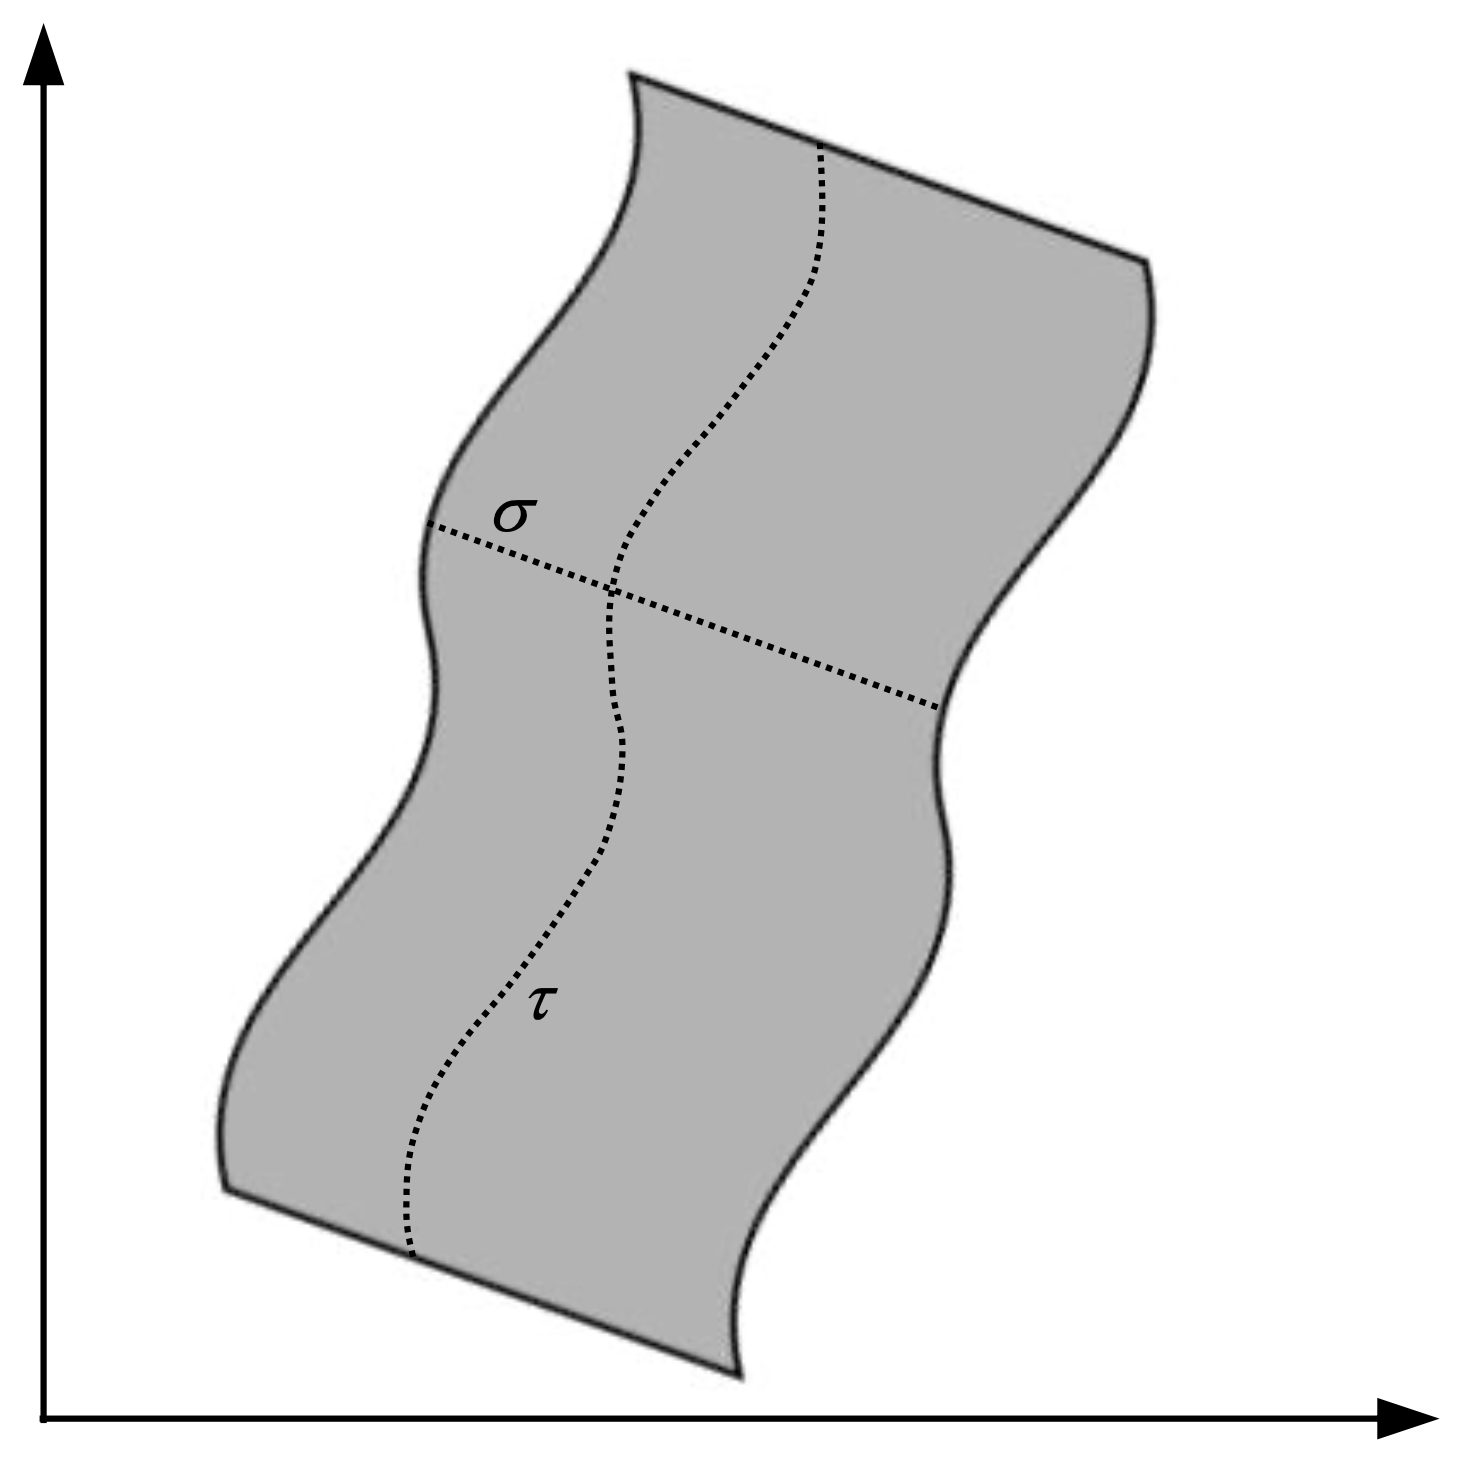
\includegraphics[scale=1]{boundary.pdf}
\caption{The open string world-sheet parameterized by $\tau$ and $\sigma$.}	
\end{figure}


The difference between open and closed string world-sheetis that they have different boundary conditions, the closed string must satisfy the periodic boundary condition $X^{\mu}(\tau,\sigma+\pi)=X^{\mu}(\tau,\sigma)$, the open string case is more complicated and we will discussion it later.

The action we have construct for $p$-brane seems a little abstract if you are not familiar with differential geometry. Now let us take the world-sheetcase as a concrete example to make you feel more comfortable with it. For the world sheet, we are concerning about the area element of the world sheet. Let us check here that 
$\sqrt{-\det G_{\alpha\beta}}d\sigma d\tau$ is actually the area element. This can be done more conveniently in Euclidean space $\mathbb{R}^D$, the philosophy is completely the same for Minkowski space. For a parameterized surface $\mathbf{X}(\tau,\sigma)=(X^1(\tau,\sigma),\cdots, X^D(\tau,\sigma))$ in  $\mathbb{R}^D$, two linearly independent tangent vectors are 
\begin{equation}
d\mathbf{u}=\partial_{\tau}\mathbf{X}d\tau,\quad d\mathbf{v}=\partial_{\sigma}\mathbf{X}d\sigma.
\end{equation}
The area element expanded by $d\mathbf{u}$ and $d\mathbf{v}$ are $dA=|d\mathbf{u}\times d\mathbf{v}|=|\mathbf{u}||\mathbf{v}|\sin \theta d\tau d\sigma$.
Recall that the induced metric on world-sheetis 
\begin{equation}
G_{\alpha\beta}=\partial_{\alpha}\mathbf{X}\cdot \partial_{\beta}\mathbf{X}=\left(\begin{array}{cc}\mathbf{u}^2 & \mathbf{u}\cdot\mathbf{v} \\ \mathbf{v}\cdot\mathbf{u} & \mathbf{v}^2\end{array}\right).
\end{equation}
We see that 
\begin{align}
\sqrt{\det G_{\alpha\beta}}d\sigma d\tau&= \sqrt{\mathbf{u}^2\mathbf{v}^2-(\mathbf{u}\cdot \mathbf{v})^2}d\sigma d\tau=\sqrt{\mathbf{u}^2\mathbf{v}^2(1-\cos^2\theta)}\nonumber\\
&=|\mathbf{u}||\mathbf{v}|\sin \theta d\tau d\sigma=dA,
\end{align}
which shows the consistency of the the area element. In Minkowski spacetime, since the induced metric  $G_{\alpha\beta}$ is not positive, thus minus sign is introduced
\begin{equation}
dA=\sqrt{-\det G_{\alpha\beta}}d\sigma d\tau.
\end{equation}

Now let us introduce the notation
\begin{align}
&\dot{X}^{\mu}=\partial_{\tau}X^{\mu}, \quad {X^{\mu}}'=\partial_{\sigma}X^{\mu}.
\end{align}
The induced metric of world-sheetcan then be written as
\begin{equation}
G_{\alpha\beta}=\left(\begin{array}{cc}\dot{X}^2 & \dot{X}\cdot X' \\ \dot{X}\cdot X'  & {X'}^2\end{array}\right).
\end{equation}
The Nambu-Goto action can be written as
\begin{equation}
\boxed{S_{NG}=-T\int d\sigma^2 \sqrt{(\dot{X}\cdot X' )^2-\dot{X}^2 {X'}^2}}
\end{equation}

The string tension $T$ is the mass per unit length, it has a close relationship with the universal Regge slop $\alpha'$ and string scale $l_{\mathrm{s}}$,
\begin{equation}
T=\frac{1}{2\pi \alpha'},\quad l_{\mathrm{s}}^2=2\alpha'.
\end{equation}
Since the spacetime coordinates has dimension $[X^{\mu}]=[\text{length}]=[\text{time}]$, thus the world-sheetcoordinates $\tau,\sigma$ are dimensionless. From the dimension of $T$ we see that $[\alpha]=[\text{length}]^2$, thus $l_{\mathrm{s}}$ has the unit of length. Length scale $l_{\mathrm{s}}$ is the natural length in string theory, and in some sense, it is the only parameter of the string theory.



\subsection{Symmetries of Nambu-Goto action}

\begin{itemize}
	\item The Nambu-Goto action has a global symmetry, Poincar\'{e} symmetry of the spacetime: $X^{\mu}\to \Lambda^{\mu}_{\nu}X^{\nu}+c^{\mu}$. In world-sheet coordinates, this means that Poincar\'{e} transformation $\Lambda_{\mu\nu}$ and $c^{\mu}$ do not depends on world-sheet coordinates $\sigma^{\alpha}$.

\item Another symmetry is the reparameterization invariance, which is a gauge symmetry. 
This reflects the fact that there is a redundancy of our description of the theory, \emph{viz.}, world-sheet coordinates have no physical meaning.
\end{itemize}


\subsection{Equation of motion and boundary conditions}
As we usually do in field theory, it is convenient for us to introduce the momenta
\begin{align}
&\mathcal{P}_{\mu}^{\tau}=\frac{\partial \mathcal{L}}{\partial \dot{X}^{\mu}}
=-T \frac{(\dot{X} \cdot X^{\prime}) X_{\mu}^{\prime}-(X^{\prime 2}) \dot{X}_{\mu}}{\sqrt{(\dot{X} \cdot X^{\prime})^{2}-\dot{X}^{2} X^{\prime 2}}},\\
&\mathcal{P}_{\mu}^{\sigma}=\frac{\partial \mathcal{L}}{\partial X^{\prime \mu}}
=-T \frac{(\dot{X} \cdot X^{\prime}) \dot{X}_{\mu}-(\dot{X}^{2}) X_{\mu}^{\prime}}{\sqrt{(\dot{X} \cdot X^{\prime})^{2}-\dot{X}^{2} X^{\prime 2}}}.
\end{align}
The equation of motion is 
\begin{equation}
\partial_{\tau}	\mathcal{P}_{\mu}^{\tau}+\partial_{\sigma}\mathcal{P}_{\mu}^{\sigma}=0.
\end{equation}
It's easily checked that, the equation of motion can be rewritten as
\begin{equation}
\partial_{\alpha}\sqrt{-\det G}G^{\alpha\beta}\partial_{\beta}X^{\mu},	
\end{equation}
where $G^{\alpha\beta}$ is the inverse of the induced metric $G_{\alpha\beta}$,
\begin{equation}
G^{\alpha\beta}=\frac{1}{(-\dot{X} \cdot X^{\prime})^{2}+\dot{X}^{2} X^{\prime 2}}\left(\begin{matrix}
 X'\cdot X' & -\dot{X}\cdot X' \\
 -X'\cdot \dot{X} & \dot{X}\cdot \dot{X}
\end{matrix}
	\right).
\end{equation}

The equation of motion looks terrible, since it is highly non-linear, so we won's solve it here but instead introduce some new equivalent action and solve the new simplified equation of motion.

The boundary conditions are also very crucial in string theory. As for the usual partial differential equations, there are several different types of boundary conditions. But here we must ask what kind of boundary conditions are physically meaningful.
For closed string the boundary condition is periodicity condition, i.e., $X^{\mu}(\tau,\sigma+\pi)=X^{\mu}(\tau,\sigma)$.

For open string, there two different types of boundary condition: 
\begin{itemize}
\item Neumann boundary condition.\index{Neumann boundary condition}
    \begin{equation}
    	  \partial_{\sigma}X^{\mu}=0, \quad \text{at}\,\, \sigma=0,\pi.
    \end{equation}
Since there is no restriction of the string endpoints $\delta X^{\mu}(\sigma=0,\pi)$, the endpoints can move freely. As we will see later, this constraint means that the endpoint of the string moves with speed of light.
 
\item Dirichlet boundary condition. \index{Dirichlet boundary condition}
 \begin{equation}
 \delta X^{\mu}=0,	\quad \text{at}\,\, \sigma=0,\pi.
 \end{equation}
This means that the string endpoints lie at some fixed position in space, i.e., $X^{\mu}(\sigma=0)=X^{\mu}_0$ and $X^{\mu}(\sigma=\pi)=X^{\mu}_{\pi}$.
\end{itemize}



\section{The Polyakov action}
The Nambu-Goto action is a straightforward generalization of the relativistic point particle action. 
For the action of relativistic point particle, we have seen that to overcome the shortcoming of the action that there is a square-root which makes it difficult to do quantization and to include the massless case, an equivalent action, einbein field action is introduced.
Similarly, we can construct an equivalent action to Nambu-Goto action, known as Polyakov action\footnote{The action is 
was discovered by Brink, Di Vecchia and Howe and by Deser and Zumino, but Polyakov understood how to do path integral with this action, thus the action is is named after him. The path integral will be discussed later in this lecture note.}, or string sigma action, which eliminates the square-root at the expense of introducing another field $h_{\alpha\beta}$. This new field $h_{\alpha\beta}$ is a dynamical metric of the world-sheet, its inverse matrix is denoted as $h^{\alpha\beta}$. The Polyakov action reads
\begin{equation}
\boxed{
S=-\frac{T}{2}	\int d\sigma^2 \sqrt{-\det h_{\alpha\beta}}h^{\alpha\beta}\partial_{\alpha}X\cdot \partial_{\beta}X. }
\end{equation}
Notice that we will frequently denote $\det h_{\alpha\beta}$ simply by $h$ whenever there is no risk to make ambiguity.

In fact, although the square-root is now eliminated, the action still looks nasty because of its complexity. In this section, we will try to simplify the analysis of the physics of this action using the its gauge symmetry. As you will see, the final result is really satisfactory, the equation of motion becomes our familiar wave equations plus some constraints given by energy-momentum tensor.


\subsection{The equation of motion}

From simple calculation, the equation of motion for $X^{\mu}$ is
\begin{equation}
\partial_{\alpha}(\sqrt{-\det h} h^{\alpha\beta}\partial_{\beta}X^{\mu})=0,	
\end{equation}
which has the same form as the equation of motion for Nambu-Goto action, but now $h_{\alpha\beta}$ is an independent field which has its own equation of motion.



To derive the equation of motion of the metic $h^{\alpha\beta}$, we need a formula about the variation of the determinant of a matrix $M$:
\begin{equation}
\delta\, \mathrm{det} M= \mathrm{det}\, M \mathrm{tr} (M^{-1}\delta M)=- \mathrm{det}\, M \mathrm{tr} (M\delta M^{-1}).
\end{equation}
Which you may have seen in relativity course, it can be prove in several different ways, we leave it as an exercise.
\begin{exercise}
Prove that for a matrix $M$, the variation of its determinant is of the following form
\begin{equation}
\delta\, \mathrm{det} M= \mathrm{det}\, M \mathrm{tr} (M^{-1}\delta M)=- \mathrm{det}\, M \mathrm{tr} (M\delta M^{-1}).
\end{equation}
\end{exercise}
Using the formula for the variation of the determinant, we have 
\begin{equation}
\delta \sqrt{-\det h}=-\frac{1}{2}\sqrt{-\det h} h_{\alpha\beta}\delta h^{\alpha\beta}=\frac{1}{2}\sqrt{-\det h} h^{\alpha\beta}\delta h_{\alpha\beta}.
\end{equation}
Notice that there is no terms involving world-sheet derivatives of the field $h^{\alpha\beta}$ in the Polyakov action, thus the equation of motion is $\delta \mathcal{L}/\delta h^{\alpha\beta}=0$. 
We will see that this is equivalent to the vanishing of the energy-momentum tensor $T_{\alpha\beta}$.

\subsubsection*{Energy-momentum tensor}

There are two different ways to calculate the energy-momentum tensor here. The first one is the usual Noether current method which you may have been familiar from the quantum field course. 
This is usually used for the situation where the spacetime is flat, i.e., no gravity.
Another way, usually appears in general relativity course, is the Hilbert energy-momentum tensor. This is usually used for the action involving gravity.

%Consider a small translation of the world sheet coordinates
%$\sigma^{\alpha}\to {\sigma'}^{\alpha}=\sigma^{\alpha}+\delta \sigma^{\alpha}$,	 the fields $X^{\mu}$ and $h_{\alpha\beta}$
%changes as
%\begin{equation}
% {X'}^{\mu}(\sigma')=X^{\mu}(\sigma),\quad h'_{\alpha\beta}=\frac{\partial x^{\rho}}{\partial{x'}^{\alpha}}	\frac{\partial x^{\sigma}}{\partial{x'}^{\beta}} h_{\rho\sigma}.
%\end{equation}
%The variation of the action $S=\int d\sigma^2 \mathcal{L}[X(\sigma),h_{\alpha\beta}(\sigma)]$ is 
%\begin{equation}
%\delta S=\int d\sigma^2 \partial^{\alpha}\left( 
%\frac{\partial \mathcal{L}}{\partial \partial^{\alpha}X^{\mu}}\delta X_{\mu} +  \frac{\partial \mathcal{L}}{\partial \partial^{\alpha}h_{\rho\sigma}}\delta h_{\rho\sigma}-T_{\alpha\beta}\delta \sigma^{\beta}
%\right),
%\end{equation}
%where the energy-momentum tensor is
%\begin{equation}
%T_{\alpha\beta}=\frac{\partial \mathcal{L}}{\partial\partial^{\alpha}X^{\mu}}\partial_{\beta}X^{\mu}	+\frac{\partial \mathcal{L}}{\partial\partial^{\alpha}h_{\rho\sigma}}\partial_{\beta}h_{\rho\sigma}	-\eta_{\alpha\beta}\mathcal{L}.
%\end{equation}

Since the Polyakov action contains the world-sheet gravity $h^{\alpha\beta}$, it is more convenient to use the Hilbert energy-momentum tensor.
By definition, the Hilbert energy-momentum tensor is of the form
\begin{equation}
\boxed{
	T_{\alpha\beta}=-\frac{2}{T}\frac{1}{\sqrt{-\det h}}\frac{\delta \mathcal{L}}{\delta h^{\alpha\beta}},}
\end{equation}
where $\frac{1}{\sqrt{-\det h}}$ is introduced as a normalization factor. 

Using the formula for variation of the determinant of a matrix, we obtain
\begin{equation}
\frac{\delta\mathcal{L}}	{\delta h^{\alpha\beta}}=-\frac{T}{2}(\sqrt{-\det h}\partial_{\alpha}X\cdot\partial_{\beta}X-\frac{1}{2}\sqrt{-\det h}h_{\alpha\beta}h^{\rho\sigma}\partial_{\rho}X\cdot\partial_{\sigma}X)=0.
\end{equation}
This implies that $h_{\alpha\beta}=f(\sigma)\partial_{\alpha}X\cdot\partial_{\beta}X=f(\sigma) G_{\alpha\beta}$ with $f(\sigma)=2/(h^{\rho\sigma}\partial_{\rho}X\cdot\partial_{\sigma}X)$. 
Substituting the expression into the the equation of motion of $X^{\mu}$, the factor $f(\sigma)$ drops out, we obtain the equation of motion for Nambu-Goto action.


The energy-momentum tensor reads
\begin{equation}
	T_{\alpha\beta}=\partial_{\alpha}X\cdot\partial_{\beta}X-\frac{1}{2}h_{\alpha\beta}h^{\rho\sigma}\partial_{\rho}X\cdot\partial_{\sigma}X.
\end{equation}
The equation of motion for $h^{\alpha\beta}$ is equivalent to $T_{\alpha\beta}=0$.



\subsection{Symmetries of the Polyakov action}
There are three symmetries of the Polyakov action:
\begin{itemize}
\item Global Poincar\'{e} symmetry: $X^{\mu}\to \Lambda^{\mu}_{\,\,\,\nu}X^{\nu}+A^{\mu}$ and $h_{\alpha\beta}$ remains unchanged.
Here, the term ``global" means that $\Lambda^{\mu}_{\,\,\,\nu},A^{\mu}$ do not depend on the world-sheet coordinates.
\item Local diffeomorphism of the world-sheet (or reparameterization invariance). This is a gauge symmetry, which indicates that world-sheet coordinates do not have physical meaning. 
Consider the transformation $\sigma \to \sigma'=\sigma'(\sigma)$, under which, we have
\begin{equation}
\begin{cases}
	X^{\mu}(\sigma)\to {X'}^{\mu}(\sigma') =X^{\mu}(\sigma'),\\
	h_{\alpha\beta}(\sigma)\to  {h'}_{\alpha\beta}(\sigma')=
	\frac{\partial \sigma^{\rho}}{\partial {\sigma'}^{\alpha}}
	\frac{\partial \sigma^{\sigma}}{\partial {\sigma'}^{\beta}} 
	h_{\rho\sigma}(\sigma).
\end{cases}	
\end{equation}
Substituting them into the action, we find that the action remains unchanged.
In some situation, it will be convenient to work infinitesimally. Consider the infinitesimal transformation $\sigma'=\sigma-\eta(\sigma)$ for some small $\eta(\sigma)$.
The transformations of the fields then become,
\begin{equation}
\begin{cases}
	\delta X^{\mu}(\sigma)=\eta^{\alpha} \partial_{\alpha} X^{\mu} \\
\delta h_{\alpha \beta}(\sigma)=\nabla_{\alpha} \eta_{\beta}+\nabla_{\beta} \eta_{\alpha}
\end{cases}
\end{equation}
where the covariant derivative is defined by $\nabla_{\alpha} \eta_{\beta}=\partial_{\alpha} \eta_{\beta}-\Gamma_{\,\,\,\alpha \beta}^{\sigma} \eta_{\sigma}$ with Christoffel symbol of the Levi-Civita connection associated to the world-sheet metric given by the usual expression,
\begin{equation}
\Gamma_{\,\,\,\alpha \beta}^{\sigma}=\frac{1}{2} h^{\sigma \rho}\left(\partial_{\alpha} h_{\beta \rho}+\partial_{\beta} h_{\rho \alpha}-\partial_{\rho} h_{\alpha \beta}\right).
\end{equation}




\item Weyl symmetry. Let us first give some comments about the name
for convenience of our later use.
Weyl symmetry or Weyl invariance is usually defined for field theory which is coupled with a background metric $g_{\mu\nu}$.
For such theories, Weyl transformations are defined as a local rescaling of the metric together with a transformation of the local operators. For primary scalar operators $\mathcal{O}$ the transformation is
\begin{equation}
\text { Weyl: } 
\begin{cases}
 g_{\mu \nu}(x) \to \Omega^{2}(x) g_{\mu \nu}(x) \\
\mathcal{O}(x)  \to \Omega^{-\Delta_{\mathcal{O}}}(x) \mathcal{O}(x)
\end{cases}
\end{equation}
where $\Omega(x)$ is an arbitrary non-vanishing function of background manifold (in quantum field theory, the spacetime manifold, in string theory, the world-sheet coordinate manifold), and $\Delta_{\mathcal{O}}$ is the dimension the operator $\mathcal{O}$.
There is a closely related but somehow different notion, conformal invariance, which will be discussed in detail in the following chapters.
Actually, many authors use two nomenclatures to mean the same thing. Here, we stress that conformal transformations are special Weyl transformations such that the transformed metric is diffeomorphic to the original metric:
\begin{equation}
\text{Conformal:}	
\begin{cases}
g_{\mu \nu}(x)  \mapsto \Omega^{2}(x) g_{\mu \nu}(x)=g_{\mu \nu}^{\prime}(x) \\
\mathcal{O}(x) \mapsto \Omega^{-\Delta_{\mathcal{O}}}(x) \mathcal{O}(x)
\end{cases}
\end{equation}

where $g_{\mu \nu}^{\prime}$ is diffeomorphic to $g_{\mu \nu}$
\begin{equation}
g_{\mu \nu}^{\prime}\left(x^{\prime}\right)=\frac{\partial x^{\rho}}{\partial x^{\prime \mu}} \frac{\partial x^{\sigma}}{\partial x^{\prime \nu}} g_{\rho \sigma}(x).
\end{equation}

At this stage, you may feel confused about these stuffs, we recommend you to turn back to read these statements after you have read the conformal field theory chapter. 

For the Polyakov action, the scalar field $X^{\mu}$ is coupled with the world-sheet metric $h_{\alpha\beta}$, the action has the Weyl symmetry.
Under the Weyl transformation
\begin{equation}
X^{\mu}(\sigma)\to	X^{\mu}(\sigma)
\end{equation}
while the metric transforms as
\begin{equation}
h_{\alpha\beta}(\sigma)\to \Omega^2(\sigma)h_{\alpha\beta}=e^{2\phi(\sigma)}h_{\alpha\beta}(\sigma).	
\end{equation}
It's easy to check that the Polyakov action is invariant under this transformation, since $h_{\alpha\beta}$ is $2\times 2$ matrix, the factor $\Omega^2(\sigma)$ drops out, canceling between $\sqrt{-\det h}$ and the inverse matrix $h^{\alpha\beta}$. Notice that this holds only for $2d$ world-sheet manifold. The Weyl symmetry is a local gauge symmetry, thus it can be used to gauge away the unphysical degrees of freedom of the theory.
\end{itemize}
 


\subsection{Conformal gauge}
The Polyakov action looks nasty to deal with, so we expect to simplify the action using the gauge symmetry. There are three local gauge symmetries: two local diffeomorphisms and one Weyl symmetry. The action has $D$ independent variables $X^{\mu}$ and three independent variables $h_{00},h_{01}=h_{10},h_{11}$.


First, let us consider the two local diffeomorphism symmetries. They can reduce the three independent variables of $h_{\alpha\beta}$ into one independent variables. Specifically, we can choose the use the following gauge choice, known as \emph{conformal gauge}:
\begin{equation}
h_{\alpha\beta}=e^{2\phi(\sigma)}\eta_{\alpha\beta}.
\end{equation}

We have another local gauge symmetry, Weyl symmetry, using which we can remove the last independent component. By setting $\phi=0$, we can fix the $h_{\alpha \beta}$ completely as
\begin{equation}
h_{\alpha \beta}=\left(\begin{array}{cc}
-1 & 0 \\
0 & 1
\end{array}\right)
\end{equation}
We end up with a flat metric, which is, of course, a good news for us.

Actually such a flat worldsheet metric is only possible if there is no topological obstruction. This is the case when the worldsheet has a vanishing Euler characteristic, e.g., a cylinder and a torus. In general, one can only do this in a given coordinate patch (not a point), for a given world-sheet manifold, we can do this in each given patch.

When a flat worldsheet metric is an allowed gauge choice (almost always done in a given coordinate patch), the Polyakov action takes the simple form
\begin{equation}
S_{\sigma}=-\frac{T}{2} \int d^{2} \sigma \partial^{\alpha} X \cdot \partial_{\alpha} X=\frac{T}{2} \int d^{2} \sigma\left(\dot{X}^{2}-X^{\prime 2}\right)
\end{equation}
Here it seems the world-sheet dynamical metric disappears, but you should always remember that it actually exists and is set as flat metric, and the equation of motion of the metric reflects in the constraint of vanishing energy-momentum tensor.

The equation of motion for $X^{\mu}$ now becomes 
\begin{equation}
\partial^{\alpha}\partial_{\alpha}X^{\mu}=0, \quad \text{or}, \quad  \left(\partial_{\sigma}^2-\partial_{\tau}^2\right)X^{\mu}=0,
\end{equation}
which is nothing but the usual wave equation.
This is of course not equivalent to the original complex form of the equation of motion for $X^{\mu}$.
We need to add the constraint that $T_{\alpha\beta}=0$. In our gauge choice, we have the following constraint
\begin{equation}
T_{01}=T_{10}=\dot{X} \cdot X^{\prime}=0 \quad \text{and} \quad T_{00}=T_{11}=\frac{1}{2}\left(\dot{X}^{2}+X^{\prime 2}\right)=0.	
\end{equation}

Let us take a close look at the constraints $T_{\alpha\beta}=0$.
The first constraint $T_{01}=T_{10}=\dot{X}\cdot X'=0$ means that the $\sigma=\text{const.}$ line and the $\tau=\text{const.}$ in world-sheet are orthogonal to each other. The other ones will be discussed use an example.

\subsection{Boundary conditions}
As we have pointed out before, for closed string, the boundary conditions is $X^{\mu}(\tau,\sigma+\pi)=X^{\mu}(\tau,\sigma)$. For open strings, there are two basic boundary conditions we can impose on endpoints of the string: 
\begin{itemize}
\item Neumann boundary condition $\partial_{\sigma}X^{\mu}\big{|}_{\sigma=0 \,\,\text{or}\,\, \pi}=0$. This is appropriate for the free string endpoint. Since we have $\mathcal{P}_{\sigma}^{\mu}=\frac{\partial \mathcal{L}}{\partial {X'}^{\mu}}=T{X'}^{\mu}$. This kind of boundary condition means that there is no momentum flow off of the endpoints of the string. 
\item Dirichlet boundary condition $\delta X^{\mu}\big{|}_{\sigma=0 \,\,\text{or}\,\, \pi}$ or equivalently $\mathcal{P}_{\tau}\big{|}_{\sigma=0 \,\,\text{or}\,\, \pi}=\frac{\partial \mathcal{L}}{\dot{X}^{\mu}}\big{|}_{\sigma=0 \,\,\text{or}\,\, \pi}=0$. This means that the ends of the string are fixed in spacetime.
\end{itemize}

Although, we learn from partial differential equation course that that are many other boundary conditions we can impose on the wave equations, however, these boundary conditions are of great importance in string theory, we won't discuss them here.


\section{Mode expansions of the string}
In the last section, we have seen that the equations of motion for Polyakov action in flat gauge are
\begin{align}
&\text{for}\,\, X^{\mu}:\quad & \partial_{\sigma}^2X^{\mu}-\partial^2_{\tau}X^{\mu}=0;\label{eq:eqm1}\\
&\text{for}\,\, h^{\alpha\beta}: \quad &T_{00}=T_{11}=\frac{1}{2}(\dot{X}^2+X'^2)=0, \label{eq:eqm2}\\
& &T_{01}=T_{10}=\dot{X}\cdot X'=0.\label{eq:eqm3}
\end{align}
We will treat these two kind of constraints separately. Firstly, we give the general solution of (\ref{eq:eqm1}) in the Fourier expansion form with coefficient undermined, 
which is known as \emph{mode expansion} \index{mode expansion} or \emph{oscillator expansion} \index{oscillator expansion} and the constraints  (\ref{eq:eqm2}) and (\ref{eq:eqm3}), known as \emph{Virasoro constraints} \index{Virasoro constraint}, are added later to the Fourier coefficients of the general solution.


As you may have seen before, the wave equation
$\partial_{\sigma}^2X^{\mu}-\partial^2_{\tau}X^{\mu}=0$
can be solved with d'Alembert method by introducing a new kind of variables $\sigma^+=\tau+\sigma$ and $\sigma^-=\tau-\sigma$, which, in string theory, are known as world-sheet light-cone coordinates. 
In terms of light-cone coordinates, we have
\begin{equation}
\partial_+=\frac{1}{2}(\partial_{\tau}+\partial_{\sigma}), \,\,\,\partial_{-}=\frac{1}{2}(\partial_{\tau}-\partial_{\sigma}),
\end{equation}
and the equation of motion simply read
\begin{equation}
\partial_+\partial_{-}X^{\mu}=0.
\end{equation}
The general solution of the equation is 
\begin{equation}
X^{\mu}(\tau,\sigma)=X_R^{\mu}(\sigma^-)+X_L^{\mu}(\sigma^+),
\end{equation}
where $X_R^{\mu}(\sigma^-)$ and $X_L^{\mu}(\sigma^-)$ are two arbitrary functions which corresponds to the right-moving waves and left-moving waves respectively, they can be expressed in the following general form
\begin{align}
X_{R}^{\mu}(\sigma^-)=\frac{x^{\mu}}{2}+\frac{l_{\mathrm{s}}^{2} p^{\mu}}{2}\sigma^{-}+\frac{i l_{\mathrm{s}}}{{2}} \sum_{k \neq 0} \frac{\alpha_{k}^{\mu}}{k} e^{-i k\sigma^{-}}, \label{eq:generalsolution1}\\
X_{L}^{\mu}(\sigma^+)=\frac{x^{\mu}}{2}+\frac{l_{\mathrm{s}}^{2} \tilde{p}^{\mu}}{2}\sigma^{+}+\frac{i l_{\mathrm{s}}}{{2}} \sum_{k \neq 0} \frac{\tilde{\alpha}_{k}^{\mu}}{k} e^{-i k\sigma^{+}}.\label{eq:generalsolution2}
\end{align}
The $\alpha_{k}^{\mu}$ and $\tilde{\alpha}_{k}^{\mu}$ are arbitrary Fourier expansion coefficients. Since the field $X^{\mu}(\tau, \sigma)$ must be real, $x^{\mu}, p^{\mu},$ and $\bar{p}^{\mu}$ must also be real and we may also derive the following reality condition for the $\alpha_k^{\mu}$ and $\tilde{\alpha}_k^{\mu}$:
\begin{equation}
\left(\alpha_{k}^{\mu}\right)^{*}=\alpha_{-k}^{\mu} \quad \text { and } \quad\left(\bar{\alpha}_{k}^{\mu}\right)^{*}=\bar{\alpha}_{-k}^{\mu}
\end{equation}
The expression is well-designed for the convenience of the quantization, as you will see in the next chapter.

To determine the exact solution, we must add the boundary condition constraints. 
We will discuss separately the cases for closed string, \emph{viz}. the periodic boundary conditions; 
and the open string with  (i) Neumann boundary conditions; (ii) Dirichlet boundary conditions; and (iii) mixed boundary conditions. The general solution takes a well-designed form of Fourier expansion such that it is convenient for quantization, this kind of expansions are know as mode expansions or oscillator expansions. 

Before we start, let us first take a quick aside to give a short comment about the convention of differential form and small displacement.
 We will take the convention that ${d}x{d}y:=\mathrm{d}x\wedge \mathrm{d}y$.
This means ${d}\tau {d}\sigma\neq {d}\sigma {d}\tau$. And sometimes we will also use the notation $\mathrm{d}x\mathrm{d}y$ to mean $\mathrm{d}x\otimes \mathrm{d}y$, e.g., for metric $d^2s=g_{\mu\nu}\mathrm{d}x^{\mu}\mathrm{d}x^{\nu}:=g_{\mu\nu}\mathrm{d}x^{\mu}\otimes\mathrm{d} x^{\nu}$.
Rigorously speaking, italic `$d$' means an infinitesimal displacement, 
e.g., $d^2s$
and romanic `$\mathrm{d}$' means a differential form. But we will take the risk to neglect this difference hereinafter as many authors do, each time when you meet it, stop and think to make the meaning clear. 
Here for light-cone coordinates, the expression may $d\sigma^+d\sigma^-$ will be used to mean $\mathrm{d}\sigma^+\wedge \mathrm{d}\sigma^-$ and $\mathrm{d}\sigma^+\mathrm{d}\sigma^-$ will be used to mean $d\sigma^+\otimes\sigma^-$. Similarly for other coordinates transforms.
The metric in world-sheet light-cone coordinates is
\begin{equation}
\tilde{h}_{\alpha\beta}=\left(\begin{array}{cc}
0 & -\frac{1}{2}\\
-\frac{1}{2} & 0
\end{array}	\right),\quad  \tilde{h}^{\alpha\beta}=\left(\begin{array}{cc}
0 & -{2}\\
-{2} & 0
\end{array}	\right).
\end{equation}
Thus, we have $\sigma_+=-\sigma^-/2$ and $\sigma_-=-\sigma^+/2$.


\subsection{Closed string case}
For the closed string, $X^{\mu}(\tau,\sigma+\pi)=X^{\mu}(\tau,\sigma)$, since it's periodic, if we impose the condition on the general solution (\ref{eq:generalsolution1}) and (\ref{eq:generalsolution2}), we must have $k\in 2\mathbb{Z}$ and $\tilde{p}^{\mu}=p^{\mu}$. By redefining the $\alpha_k^{\mu}$ and $\tilde{\alpha}_k^{\mu}$, we obtain the following mode expansion for closed string:
\begin{svgraybox}
\begin{align} 
X_{R}^{\mu}(\sigma^-)=\frac{1}{2}x^{\mu}+\frac{1}{2}l_{\mathrm{s}}^2p^{\mu}\sigma^{-}+\frac{1}{2}il_{\mathrm{s}}\sum_{n\neq 0}\frac{1}{n}\alpha_{n}^{\mu}e^{-2in\sigma^{-}},\label{eq:mxpR}\\
X_{L}^{\mu}(\sigma^+)=\frac{1}{2}x^{\mu}+\frac{1}{2}l_{\mathrm{s}}^2p^{\mu}\sigma^{+}+\frac{1}{2}il_{\mathrm{s}}\sum_{n\neq 0}\frac{1}{n}\tilde{\alpha}_{n}^{\mu}e^{-2in\sigma^{+}}. \label{eq:mxpL}
\end{align}
\end{svgraybox}

Here $x^{\mu}$ and $p^{\mu}$ are center-of-mass position and momentum as we will check later. The requirement that $X_R^{\mu}(\sigma^-)$ and $X_L^{\mu}(\sigma^-)$ are real implies that $x^{\mu}$ and $p^{\mu}$ are real and
\begin{equation}
\alpha_{-n}^{\mu}=(\alpha_{n}^{\mu})^*,\,\,\,\tilde{\alpha}_{-n}^{\mu}=(\tilde{\alpha}_{n}^{\mu})^*. 
\end{equation}

We also recall here that $l_{\mathrm{s}}^2=2\alpha'$ and $T=1/(2\pi\alpha')$. If we set $\alpha_0^{\mu}=\tilde{\alpha}_{0}^{\mu}=l_{\mathrm{s}}p^{\mu}/2$, the derivatives of the mode expansion take the form
\begin{align}
\partial_{-}X_R^{\mu}(\sigma^{-})=l_{\mathrm{s}}\sum_{m\in \mathbb{Z}}\alpha^{\mu}_ne^{-2in\sigma^{-}},\label{eq:pplus}\\
\partial_{+}X_L^{\mu}(\sigma^{+})=l_{\mathrm{s}}\sum_{m\in \mathbb{Z}}\tilde{\alpha}^{\mu}_ne^{-2in\sigma^{+}}\label{eq:minus}.
\end{align}
From the above equalities, the derivatives with respect to $\tau$ and $\sigma$ can easily be obtained. Recall that $\partial_{\tau}=\partial_{+}+\partial_{-}$ and $\partial_{\sigma}=\partial_{+}-\partial_{-}$, we have
\begin{align}
\dot{X}^{\mu}=\partial_{+}X_L^{\mu}(\sigma^{+})+\partial_{-}X_R^{\mu}(\sigma^{-})\label{eq:pplus1}\\
{X^{\mu}}'=\partial_{+}X_L^{\mu}(\sigma^{+})-\partial_{-}X_R^{\mu}(\sigma^{-})\label{eq:pminus1}.
\end{align}


Now let us briefly demonstrate that $x^{\mu}$ and $p^{\mu}$ are center-of-mass position and momentum. Consider $X^{\mu}(\tau,\sigma)=X_R^{\mu}(\sigma^-)+X_L^{\mu}(\sigma^+)$, the center-of-mass position is
\begin{equation}
X_{c}^{\mu}(\tau)=\frac{1}{\pi}\int_0^{\pi}d\sigma X^{\mu}(\tau,\sigma)=x^{\mu}+l_{\mathrm{s}}^2p^{\mu}\tau.
\end{equation}
Thus, $x^{\mu}$ is the center of mass at the initial time $\tau=0$ and is moving as a free particle with velocity $l_{\mathrm{s}}^2p^{\mu}$.
Since the momentum density is $\mathcal{P}^{\mu}=\delta{\mathcal{L}}/\delta \dot{X}_{\mu}=T\dot{X}^{\mu}$, the center-of-mass momentum is
\begin{align}
p^{\mu}_c(\tau)&=T\int_0^{\pi}d\sigma \dot{X}^{\mu}=Tl_{\mathrm{s}}\int_0^{\pi}d\sigma\sum_{n\in\mathbb{Z}}(\alpha^{\mu}_ne^{-2in\sigma^{-}}+\tilde{\alpha}^{\mu}_ne^{-2in\sigma^{+}})\nonumber\\
&=\frac{1}{l_{\mathrm{s}}}(\alpha_0^{\mu}+\tilde{\alpha}_0^{\mu})\equiv p_{\mu}.
\end{align}
Thus the center-of-mass momentum is a constant $p^{\mu}$, which coincide with the fact that the string is moving freely.




%==============================
\subsubsection*{Poisson bracket}
The canonical quantization of bosonic string is just a procedure to replace the classical Poisson bracket to quantum bracket. Now let us calculate the Poisson bracket for closed string mode expansion. For the $X^{\mu}$ field and the corresponding momentum $\mathcal{P}^{\mu}=T\dot{X}^{\mu}$ of Polyakov action in flat (or conformal) gauge, we have the following equal-$\tau$ Poisson bracket
\begin{align}
[X^{\mu}(\tau,\sigma),X^{\nu}(\tau,\sigma')]_{\mathrm{PB}}=[\mathcal{P}^{\mu}(\tau,\sigma),\mathcal{P}^{\nu}(\tau,\sigma')]_{\mathrm{PB}}=0,\label{eq:bpx1}\\
[X^{\mu}(\tau,\sigma),\mathcal{P}^{\nu}(\tau,\sigma')]_{\mathrm{PB}}=T[X^{\mu}(\tau,\sigma),\dot{X}^{\nu}(\tau,\sigma')]_{\mathrm{PB}}=\eta^{\mu\nu}\delta(\sigma-\sigma')\label{eq:bpx2}.
\end{align}

How does this reflect in the mode expansion coefficients? Using Eqs. (\ref{eq:pplus})-(\ref{eq:pminus1}) and by taking derivatives with respect to $\sigma,\sigma'$, the following equations arise
\begin{align}
[{X^{\mu}}'(\tau,\sigma),{X^{\nu}}'(\tau,\sigma')]_{\mathrm{PB}}=[{\dot{X}^{\mu}}(\tau,\sigma),{\dot{X}^{\nu}}(\tau,\sigma')]_{\mathrm{PB}}=0,\\
[{X^{\mu}}'(\tau,\sigma),{\dot{X}^{\nu}}(\tau,\sigma')]_{\mathrm{PB}}=\frac{1}{T}\eta^{\mu\nu}\frac{d}{d\sigma}\delta(\sigma-\sigma').
\end{align}
From the above equations, the following Poisson brackets are obtained easily
\begin{align}
[\partial_{\pm}X^{\mu}(\tau,\sigma),\partial_{\pm'}X^{\nu}(\tau,\sigma')]_{\mathrm{PB}}=\pm 2T g^{\mu\nu}\frac{d}{d\sigma}\delta(\sigma,\sigma'),\\
[\partial_{\pm}X^{\mu}(\tau,\sigma),\partial_{\mp'}X^{\nu}(\tau,\sigma')]_{\mathrm{PB}}=0.
\end{align}
Then from above Poisson brackets and expanding the Dirac delta function as $\delta(\sigma-\sigma')=\frac{1}{\pi}\sum_{n\in\mathbb{Z}}e^{-2ni(\sigma-\sigma')}$, we can compare two sides to obtain the Poisson brackets for the mode expansion coefficients.

\begin{svgraybox}
\begin{align}
[\alpha_{m}^{\mu}, \alpha_{n}^{\nu}]_{\mathrm{PB}}=[\tilde{\alpha}_{m}^{\mu}, \tilde{\alpha}_{n}^{\nu}]_{\mathrm{PB}}=-i m \eta^{\mu \nu} \delta_{m+n, 0}, \label{eq:bcoeff1}\\
[\tilde{\alpha}_{m}^{\mu}, \alpha_{n}^{\nu}]_{\mathrm{PB}}=0, \quad m, n \in \mathbb{Z},\label{eq:bcoeff2}\\
[x^{\mu}, x^{\nu}]_{\mathrm{PB}}=[p^{\mu}, p^{\nu}]_{\mathrm{PB}}=0,  [x^{\mu}, p^{\nu}]_{\mathrm{PB}}=\eta^{\mu \nu}, \\
[x^{\mu}, \tilde{\alpha}_{n}^{\nu}]_{\mathrm{PB}}=[p^{\mu}, \tilde{\alpha}_{n}^{\nu}]_{\mathrm{PB}}=0=[x^{\mu}, \alpha_{n}^{\nu}]_{\mathrm{PB}}=[p^{\mu}, \alpha_{n}^{\nu}]_{\mathrm{PB}}, \,\, n\neq 0.
\end{align}
\end{svgraybox}
\begin{exercise}
Give a detailed proof of the Poisson brackets (\ref{eq:bcoeff1})-(\ref{eq:bcoeff2}) for mode expansion coefficients from the the Poisson brackets (\ref{eq:bpx1}) and (\ref{eq:bpx2}) involve only $X^{\mu}$ and $\mathcal{P}^{\nu}$.
\end{exercise}

\subsubsection*{Virasoro modes}
Now let us consider the constraints (\ref{eq:eqm2}) and (\ref{eq:eqm3}) imposed by the equation of motion of $h^{\alpha\beta}$. In the world-sheet light-cone coordinate, they becomes
\begin{equation}
T_{++}=(\partial_{+}X)^2=(\partial_{+}X_{L})^2=0,\quad
T_{--}=(\partial_{-}X)^2=(\partial_{-}X_{R})^2=0.
\end{equation}
It's obvious that they are equivalent to (\ref{eq:eqm2}) and (\ref{eq:eqm3}). 
And the other two components vanish automatically,
\begin{align}
T_{+-}=&\partial_+X\cdot\partial_{-}X-\frac{1}{2}\tilde{h}_{+-}\tilde{h}^{\alpha\beta}\partial_{\alpha}X\cdot\partial_{\beta} X\nonumber\\
=&\partial_+X\cdot\partial_{-}X-\frac{1}{2}\times (-\frac{1}{2})(-4\partial_+X\cdot\partial_{-}X)=0.
\end{align}
Similarly for $T_{-+}$.

From the light-cone coordinates derivatives of the mode expansions (\ref{eq:pplus}) and (\ref{eq:minus}), we obtain
\begin{align}
T_{--}=(\partial_{-}X)^2&=l_{\mathrm{s}}^2\sum_{k,m\in \mathbb{Z}}\alpha_{k}\cdot\alpha_{m}e^{-2i(m+k)\sigma^-}\nonumber\\
&=l_{\mathrm{s}}^2\sum_{m,n\in \mathbb{Z}}\alpha_{n-m}\cdot\alpha_{m}e^{-2in\sigma^-}\nonumber\\
&=2l_{\mathrm{s}}^2\sum_{n\in\mathbb{Z}}L_ne^{-2in\sigma^-}=0,
\end{align}
where we have introduced a new term, called Virasoro generators
\begin{equation}
L_n=\frac{1}{2}\sum_{m\in\mathbb{Z}}\alpha_{n-m}\cdot\alpha_{m}=\frac{1}{2\pi l_{\mathrm{s}}^2}\int_{0}^{\pi}T_{--}e^{2in\sigma^-}d\sigma.
\end{equation}
Similarly, from the left moving modes contribution $T_{++}$, we introduce
\begin{equation}
\tilde{L}_n=\frac{1}{2}\sum_{m\in\mathbb{Z}}\tilde{\alpha}_{n-m}\cdot \tilde{\alpha}_{m}=\frac{1}{2\pi l_{\mathrm{s}}^2}\int_{0}^{\pi}T_{++}e^{2in\sigma^+}d\sigma.
\end{equation}
They satisfy reality condition
\begin{equation}
L_n^*=L_{-n},\quad \tilde{L}_n^*=\tilde{L}_{-n}.	
\end{equation}
The equation of motion for $h^{\alpha\beta}$ now can be expressed using the Virasoro generators as
\begin{equation}
L_n=\tilde{L}_n=0,\quad n\in \mathbb{Z}.
\end{equation}

From the Poisson brackets for the oscillator modes, we can derive the Poisson brackets for the Virasoro generators. They form an algebra known as the classical Virasoro algebra: \index{classical Virasoro algebra}
\begin{svgraybox} 
\begin{align}
&[L_{m}, L_{n}]_{P B}=-i(m-n) L_{m+n}\\
&[\tilde{L}_{m}, \tilde{L}_{n}]_{P B}=-i(m-n) \tilde{L}_{m+n}\\
&[L_{m}, \tilde{L}_{n}]_{P B}=0
\end{align}
\end{svgraybox}
\begin{exercise}
Prove the above Poisson brackets form the Poisson brackets of the mode expansion coefficients.	
\end{exercise}


\subsubsection*{Hamiltonian and energy-momentum tensor}



\subsection{Open string case}
Let us now discuss the open string case. As we have pointed out, there are three kind of combination of the boundary conditions we can impose on two ends of the string.
\subsubsection*{Neumann-Neumann (NN) boundary condition}
For the Neumann-Neumann (NN) boundary condition, we impose Neumann boundary condition on both ends of the string. Consider the general solution (\ref{eq:generalsolution1}) and (\ref{eq:generalsolution2}), 
\begin{equation}
X^{\mu}=x^{\mu}+\frac{l_{\mathrm{s}}^2}{2}(p^{\mu}\sigma^-+\tilde{p}^{\mu}\sigma^+)
+\frac{il_{s}}{2}\sum_{k\neq 0}\frac{1}{k}(\alpha_k^{\mu}e^{-ik\sigma^-}+\tilde{\alpha}_k^{\mu}e^{-ik\sigma^+}).
\end{equation}
Taking the derivative with respect to $\sigma$, we have 
\begin{align}
\partial_{\sigma}{X}^{\mu}=&	(\partial_+-\partial_{-})(X_L^{\mu}+X^{\mu}_R)\nonumber\\
=&\frac{l_{\mathrm{s}}^2}{2}(\tilde{p}^{\mu}-p^{\mu})
+\frac{l_{s}}{2}\sum_{k\neq 0}(\tilde{\alpha}_k^{\mu}e^{-ik\sigma^+}-\alpha_k^{\mu}e^{-ik\sigma^-}).
\end{align}
For $\sigma=0$, $\partial_{\sigma}{X}^{\mu}=0$
\begin{equation}
	\frac{l_{\mathrm{s}}^2}{2}(\tilde{p}^{\mu}-p^{\mu})
+\frac{l_{s}}{2}\sum_{k\neq 0}(\tilde{\alpha}_k^{\mu}-\alpha_k^{\mu})e^{-ik\tau}=0
\end{equation}
implies that $\tilde{p}^{\mu}=p^{\mu}$ and $\tilde{\alpha}_k^{\mu}=\alpha_k^{\mu}$.
Then, for $\sigma=\pi$, $\partial_{\sigma}{X}^{\mu}=0$
\begin{equation}
\frac{l_{s}}{2}\sum_{k\neq 0}{\alpha}_k^{\mu}e^{-ik\tau}(e^{-ik\pi}-e^{ik\pi})=0	
\end{equation}
implies that $k\in \mathbb{Z}$. 
In summary, we have the following mode expansion
\begin{svgraybox}
\begin{align}
\text{NN:}\quad	 X^{\mu}=x^{\mu}+l_s^2p^{\mu}\tau+il_s\sum_{n\neq 0}\frac{1}{n}\alpha_n^{\mu} e^{-in\tau} \mathrm{cos}(n\sigma)
\end{align}	
\end{svgraybox}

If we set $\alpha_0^{\mu}=l_sp^{\mu}$ (note there is a $1/2$ difference with the closed string convention), we have
\begin{equation}
\partial_{\pm}X^{\mu}=\frac{l_s}{2}\sum_{n\in\mathbb{Z}}\alpha^{\mu}_ne^{-in\sigma^{\pm}}.	
\end{equation}
The center-of-mass position is
\begin{equation}
x^{\mu}_{c}(\tau)=\frac{1}{\pi}\int_0^{\pi}d\sigma X^{\mu}=x^{\mu}+l_s^2p^{\mu}\tau	
\end{equation}
and the center-of-mass momentum is
\begin{equation}
p_c^{\mu}(\tau)=T\int_0^{\pi}d\sigma \dot{X}^{\mu}={p^{\mu}}.	
\end{equation}



\subsubsection*{Dirichlet-Dirichlet (DD) boundary condition}
In the study of $Dp$-brane, we may also encounter the Dirichlet-Dirichlet (DD) boundary, for which two ends of the string are fixed in spacetime.

Consider
\begin{align}
\partial_{\tau}X^{\mu}=	\frac{l_{\mathrm{s}}^2}{2}(\tilde{p}^{\mu}+p^{\mu})
+\frac{l_{s}}{2}\sum_{k\neq 0}(\tilde{\alpha}_k^{\mu}e^{-ik\sigma^+}+\alpha_k^{\mu}e^{-ik\sigma^-})
\end{align}
Imposing the Dirichlet boundary condition at $\sigma=0$, we have
\begin{equation}
p^{\mu}=-\tilde{p}^{\mu}	, \quad \alpha_k^{\mu}=-\tilde{\alpha}_k^{\mu}.
\end{equation}
Then for $\sigma=\pi$, the boundary condition imply that $k\in \mathbb{Z}$.
Finally, the mode expansion for DD boundary condition is (where we have redefinee $\alpha_n^{\mu}$ as $\tilde{\alpha}_n^{\mu}$ and $w^{\mu}=\tilde{p}^{\mu}$)
\begin{svgraybox}
\begin{equation}
X^{\mu}=x^{\mu}+l_s^2w^{\mu}\sigma+l_s\sum_{n\neq 0}\frac{1}{n}\alpha_n^{\mu}e^{-in\tau}\mathrm{sin} (n\sigma	).
\end{equation}
\end{svgraybox}
Notice that this expansion is completely different with the NN case and closed string case in its physical essence. One importance thing is
no momentum is allowed for DD open string, only winding is allowed. 
Therefore, we have chosen the notation $w^{\mu}$ in our mode expansion.
The two ends are fixed at $X^{\mu}(\sigma=0)=x^{\mu}$ and $X^{\mu}(\sigma=\pi)=x^{\mu}+l_s^2w^{\mu}\pi$, wee see that $w^{\mu}$ characterize the distance between two ends of the string.

\begin{exercise}
Calculate the center-of-mass position and center-of-mass momentum of the DD open string. 	
\end{exercise}


\subsubsection*{Dirichlet-Neumann (DN) boundary condition}
The final case we will discuss is a combination of the Dirichlet and Neumann (DN) boundary conditions.
The Dirichlet boundary condition at $\sigma=0$ implies that
\begin{equation}
p^{\mu}=-\tilde{p}^{\mu}	, \quad \alpha_k^{\mu}=-\tilde{\alpha}_k^{\mu}.
\end{equation}
Thus we have
\begin{equation}
	X^{\mu}=x^{\mu}+l_s^2\tilde{p}^{\mu}\sigma+\frac{il_s}{2}\sum_{k\neq 0}\frac{1}{k}(\alpha_k^{\mu}e^{-ik\sigma^-}+\tilde{\alpha}^{\mu}_ke^{-ik\sigma^+} ),
\end{equation}
and its $\sigma$-derivative is
\begin{equation}
\partial_{\sigma}X^{\mu}=l_s^2\tilde{p}^{\mu}+{il_s}\sum_{k\neq 0}\tilde{\alpha}_k^{\mu}e^{-ik\tau}\cos (k\sigma)	.
\end{equation}
Imposing the Neumann boundary condition at $\sigma=\pi$, we obtain
\begin{equation}
l_s^2\tilde{p}^{\mu}+{il_s}\sum_{k\neq 0}\tilde{\alpha}_k^{\mu}e^{-ik\tau}\cos (k\pi)=0,	
\end{equation}
which implies that
\begin{equation}
\tilde{p}^{\mu}=p^{\mu}=0, \quad 	k\in \mathbb{Z}+\frac{1}{2}.
\end{equation}
Therefore the mode expansion for DN boundary condition is (we redefine $\alpha_k^{\mu}$ as $\tilde{\alpha}^{\mu}_k$)
\begin{svgraybox}
\begin{equation}
X^{\mu}=x^{\mu}+l_s\sum_{k\in \mathbb{Z}+\frac{1}{2}}\frac{1}{k}\alpha_k^{\mu}e^{-ik\tau}\sin (k\sigma).
\end{equation}	
\end{svgraybox}
This is an open string with an given direction, the $\sigma=0$ end is fixed in spacetime and the $\sigma=\pi$ end is free to move in spacetime. 
\begin{exercise}
Calculate the center-of-mass position and center-of-mass momentum of the DN open string. 	
\end{exercise}



\chapter{Quantization of the bosonic string}

\epigraph{That which does not kill us makes us stronger.}
{\textit{By Friedrich Nietzsche\\ From the book ``Twilight of the Idols"}}





In this chapter, we will discuss how to quantize the string.



\section{Canonical quantization}

Our goal is to quantize $D$ scalar fields $X^{\mu}$ governed by the Polyakov action in conformal gauge. 
The equation of motion is $\partial_{-}\partial_{+}X^{\mu}=0$.
The constraint from the vanishing of energy-momentum tensor is
\begin{equation}
T_{--}=T_{++}=0,
\end{equation}
or equivalent, they are expressed by classical Virasoro generators
\begin{equation}
L_n=\tilde{L}_n=0,	
\end{equation}
sicne $L_n$ and $\tilde{L}_n$ are Fourier expansion coefficient of the $T_{--}$ and $T_{++}$.


The canonical way for quantization is promoting the classical fields into operators and by replacing the Poisson brackets into quantum brackets according to
\begin{equation}
[\cdot,\cdot]_{\mathrm{PB}}\to -i[\cdot,\cdot].
\end{equation}
Thus, for fields $X^{\mu}$ and its conjugate momentum $\mathcal{P}^{\mu}$ we have
\begin{align}
&[X^{\mu}(\tau,\sigma),X^{\nu}(\tau,\sigma')]=[\mathcal{P}^{\mu}(\tau,\sigma),\mathcal{P}^{\nu}(\tau,\sigma')]=0,\\
&[X^{\mu}(\tau,\sigma),\mathcal{P}^{\nu}(\tau,\sigma')]=\eta^{\mu\nu}\delta(\sigma-\sigma').
\end{align}
 As we will see, this kind of quantization scheme makes the Lorentz invariance manifest, but there will be some states with negative norm.
 
Using the mode expansion of $X^{\mu}$, we can also promote $x^{\mu}$, $p^{\mu}$ and $\alpha^{\mu}_n$ and $\tilde{\alpha}^{\mu}_n$ into operators. From the commutation relation of $X^{\mu}$ and $\mathcal{P}^{\nu}$, we obtain the commutation relations (for closed string)\footnote{We can also obtain the commutation relation by replacing the classical Poisson brackets into quantum bracket $[\cdot,\cdot]_{\mathrm{PB}}\to -i[\cdot,\cdot]$ from their classical commutation relation.}
\begin{align}
[\alpha_{m}^{\mu}, \alpha_{n}^{\nu}]=[\tilde{\alpha}_{m}^{\mu}, \tilde{\alpha}_{n}^{\nu}]=m \eta^{\mu \nu} \delta_{m+n, 0}, \label{eq:qbcoeff1}\\
[\tilde{\alpha}_{m}^{\mu}, \alpha_{n}^{\nu}]=0, \quad m, n \in \mathbb{Z},\label{eq:qbcoeff2}
\end{align}
and
\begin{align}
[x^{\mu}, x^{\nu}]=[p^{\mu}, p^{\nu}]=0,  [x^{\mu}, p^{\nu}]=i\eta^{\mu \nu}, \\
[x^{\mu}, \tilde{\alpha}_{n}^{\nu}]=[p^{\mu}, \tilde{\alpha}_{n}^{\nu}]=0=[x^{\mu}, \alpha_{n}^{\nu}]=[p^{\mu}, \alpha_{n}^{\nu}], \,\, n\neq 0.
\end{align}
For open string commutation relations remain the same, but $\tilde{\alpha}^{\mu}_n$ modes do not appear.
The commutation relations for $x^{\mu}$ and $p^{\nu}$ are expected for operators governing the position and momentum of center of mass of the string. The $\alpha^{\mu}_n$ and $\tilde{\alpha}^{\nu}_n$ are in fact
harmonic oscillator creation and and annihilation operator in disguise. Let's now  try to make it more clear.

\subsection{Fock space}
The mode expansion coefficient operator $\alpha^{\mu}_n$ and $\tilde{\alpha}^{\nu}_n$  can be regarded as the creation and annihilation operator in the following way
\begin{equation}
a_n=\frac{\alpha_{n}}{\sqrt{n}},\quad 	a_n^{\dagger}=\frac{\alpha_{-n}}{\sqrt{n}}, \quad \text{for}\,\, n>0.
\end{equation}
Here we have omitted the $\mu$ label. 
For closed string, $\tilde{\alpha}_n^{\mu}$ part can be translated into creation and annihilation operators in the same way. 
From the commutation relation of $\alpha_n^{\mu}$, we see that $[a_n,a^{\dagger}_m]=\delta_{m,n}$ which is our familiar commutator for creation and annihilation operator.


With the creation and annihilation operators in hand, we can build the Fock space by giving the vacuum state of string $|0\rangle$. Notice that the creation operator do not contain the zero mode coefficient $\alpha_{0}^{\mu}=l_{\mathrm{s}}p^{\mu}/2$, thus the the vacuum state should carry another quantum number $k^{\mu}$ which is the eigenvalue of $p^{\mu}$, we denote it as $|0;k^{\mu}\rangle$. The annihilation operator acting on vacuum state get zero value
\begin{equation}
\alpha_{n}^{\mu}|0;k^{\mu}\rangle=	\tilde{\alpha}_{n}^{\mu}|0;k^{\mu}\rangle=0,\quad \text{for}\,\,n>0.
\end{equation}
The zero mode coefficient part is given equivalently by the momentum operator
\begin{equation}
p^{\mu}	|0;k^{\mu}\rangle=k^{\mu}|0;k^{\mu}\rangle.
\end{equation}

The Fock space can then be built by acting with creation operator $\alpha_n^{\mu}$ and $\tilde{\alpha}_m^{\nu}$ with $n<0$. Each state in Fock space is an excited state of the string. The generic states are of the form
\begin{equation}
(\alpha_{m_1}^{\dagger})^{n_1}\cdots	(\alpha_{m_q}^{\dagger})^{n_q}|0;k^{\mu}\rangle,\quad \text{for}\,\, m_1,\cdots , m_q>0.
\end{equation}

As in quantum field theory, we introduce the normal order of a series of product of $\alpha_{m_1}\cdots \alpha_{m_q}$ as $:\alpha_{m_1}\cdots \alpha_{m_q}:$ for which the creation operators are on the left of the annihilation operators, and we make a further convention that all subscripts are arranged in order from small to large. For example
\begin{equation}
:\alpha_5\alpha_{-1}\alpha_{3}\alpha_0\alpha_{-3}:=\alpha_{-3}	\alpha_{-1}\alpha_0\alpha_{3}\alpha_5.
\end{equation}
The normal order will be useful later in expression of physical operators using mode coefficients.



\subsubsection*{Ghost: negative-norm states}

The Fock space we constructed has a problem, \emph{viz}., some states in the space have negative norm. The reason is that the commutation relation involving the time component filed $X^{0}$ has a minus sign:
\begin{equation}
[\alpha^{0}_m,(\alpha^{0}_n)^{\dagger}]=[\tilde{\alpha}^{0}_m,(\tilde{\alpha}^{0}_n)^{\dagger}]=\eta^{00}m\delta_{m,n}=-m\delta_{m,n},
\end{equation}
note that we have used $(\alpha_n^0)^{\dagger}=\alpha^0_{-n}$ and $(\tilde{\alpha}_n^0)^{\dagger}=\tilde{\alpha}^0_{-n}$.

Consider the norm of states $\alpha^0_{-m}|0;k^{\mu}\rangle$ with $m>0$,
\begin{equation}
\|\alpha^0_{-m}|0;k^{\mu}\rangle\|=\langle 0;k^{\mu}|\alpha_{m}^0\alpha^0_{-m}|0;k^{\mu}\rangle=\langle 0;k^{\mu}|(-m+\alpha_{-m}^0\alpha^0_{m})|0;k^{\mu}\rangle=-m.
\end{equation}
In fact, whenever there are odd number of timelike oscillator excited, the norm of the states is negative.
The states with negative norm is referred to as \emph{ghost}\index{ghost}. Physically speaking, to make the sense of the theory, we must make sure that ghosts can not be produced by any physical process.

\subsection{Virasoro algebra and physical states}
\index{Virasoro generator}
Now let us consider how to add the constraint $L_{n}=\tilde{L}_n=0$. 
It's sufficient to make the constraint that, for arbitrary physical states $|\psi\rangle$ and $|\phi\rangle$, we have
\begin{equation}
\langle \psi |L_n|\phi\rangle=0,\quad 	\langle \psi |\tilde{L}_n|\phi\rangle=0, \quad \text{for} \,\, n>0.
\end{equation}
where $n>0$ is set because of $L_{-n}=L_n^{\dagger}$, $n<0$ conditions are guaranteed by $n>0$ condition. In summary, for physical states $|\phi\rangle$, we have
\begin{equation}
L_n|\phi\rangle=\tilde{L}_n|\phi\rangle=0	.
\end{equation}
 

Now the question is how to define operators $L_n$ and $\tilde{L}_n$ and what constraint we should impose for $L_0$. We can naively guess that by directly promoting the $\alpha_n$ in the classical expression of $L_n$
\begin{equation}
L_n=\frac{1}{2}\sum_{m=-\infty}^{\infty}\alpha_{n-m}\cdot\alpha_{m}.	
\end{equation}
Unfortunately, this does not work. As in quantum field theory, we must normal-order the product of operators, thus the Virasoro generator can be defined as
\begin{equation}
L_n	=\frac{1}{2}\sum_{m=-\infty}^{\infty}:\alpha_{n-m}\cdot\alpha_{m}:,\quad \tilde{L}_n	=\frac{1}{2}\sum_{m=-\infty}^{\infty}:\tilde{\alpha}_{n-m}\cdot\tilde{\alpha}_{m}:.
\end{equation}
\begin{exercise}
	Prove that for the normal-ordering definition of $L_n$ and $\tilde{L}_n$, we have $L_{-n}=L_n^{\dagger}$ and  $\tilde{L}_{-n}=\tilde{L}_{n}^{\dagger}$.
\end{exercise}
From the definition, for $n\neq 0$, terms in expression of $L_n$   
are always commutes, $[\alpha_m^{\mu},\alpha_{n-m}^{\nu}]=m\eta^{\mu\nu}\delta_{n,0}=0$, we can change the order arbitrarily. Thus normal order definition works for our goal to set constraint $L_n=0$. 

	
However, for $n=0$, the order ambiguity issue  arises,
\begin{equation}
L_0=\frac{1}{2}\sum_{m=\infty}^{+\infty}:\alpha_{-m}\cdot\alpha_{m}:=\frac{1}{2}(\alpha_0)^2	+\sum_{m=1}^{+\infty} \alpha_{-m}\cdot \alpha_{m}
\end{equation}
where $[\alpha^{\mu}_{m},\alpha^{\nu}_{-m}]=m\eta^{\mu\nu}\eta_{m-m,0}$, they do not always commute, when we try to promote classical expression of $L_0$ into the quantum normal-ordering express, some extra constant term arise. This results in the fact that to make the quantum analogue of classical constraint $L_0=0$, we must introduce a parameter $a$, such that for physical state $|\phi\rangle$,
\begin{equation}
(L_0-a)|\phi\rangle=0.	
\end{equation}
Similar for $\tilde{L}_0$.


	In summary, the physical state conditions for closed string read
\begin{svgraybox}
\begin{align}
\left({L}_{0}-a\right)|\phi\rangle=\left(\tilde{L}_{0}-a\right)|\phi\rangle &=0 \label{eq:mass_shell}\\
{L}_{m>0}|\phi\rangle =\tilde{L}_{m>0}|\phi\rangle&=0
\end{align}
\end{svgraybox}
For open string, $\tilde{L}_n$ part vanishes. The condition (\ref{eq:mass_shell}) is often called mass-shell condition.


\subsubsection*{Mass-shell condition}
\index{mass-shell condition}
As we have discussed for classical string mode expansion, $L_0$ and $\tilde{L}_0$ play important roles in determining the spectrum of string. Recall that $\alpha_{0}^{\mu}=\tilde{\alpha}_0^{\mu}=l_{\mathrm{s}}p^{\mu}/2$, we see that
\begin{align}
-M^2=p^{\mu}p_{\mu}&=\frac{4}{l_{\mathrm{s}}^2}	\alpha_{0}\cdot \alpha_0=\frac{4}{l_{\mathrm{s}}^2}	\tilde{\alpha}_{0}\cdot \tilde{\alpha}_0\nonumber\\
&=\frac{2}{\alpha'}	\alpha_{0}\cdot \alpha_0=\frac{2}{\alpha'}	\tilde{\alpha}_{0}\cdot \tilde{\alpha}_0.
\end{align}
Using the expression of $L_0$ and $\tilde{L}_0$ and the physical state condition $L_0-a=0$ and $\tilde{L_0}-a=0$, we see that
\begin{equation}
M^2=\frac{4}{\alpha'}(-a+\sum_{m=1}^{\infty}\alpha_{-m}\cdot\alpha_{m})=\frac{4}{\alpha'}(-a+\sum_{m=1}^{\infty}\tilde{\alpha}_{-m}\cdot\tilde{\alpha}_{m})	.
\end{equation}	
We can introduce the \emph{level operator} (or \emph{number operator}, although there is a $\sqrt{m}$ difference in each term of the summation from the true number operator)
\begin{equation}
N=\sum_{m=1}^{\infty}\alpha_{-m}\cdot\alpha_{m},\quad \tilde{N}=	\sum_{m=1}^{\infty}\tilde{\alpha}_{-m}\cdot\tilde{\alpha}_{m}.
\end{equation}
The condition that for physical state $N=\tilde{N}$ is known as \emph{level matching condition}. The mass operator and level operator are related by
\begin{equation}
M^2=\frac{4}{\alpha'}(N-a)=\frac{4}{\alpha'}(\tilde{N}-a).	
\end{equation}






\subsubsection*{Virasoro algebra}



The quantum expression of Virasoro generators satisfy the commutation relation
\begin{equation}\label{eq:qvirasoro}
[L_m,L_n]=(m-n)L_{m+n}+\frac{c}{12}m(m^2-1)\delta_{m+n,0},	
\end{equation}
where $c=D$ is the spacetime dimension. This can be proved using the commutation relation of $\alpha_n^{\mu}$. Similar for $\tilde{L}_n$.
Here $c$ is called central charge, which is absent in classical commutation relations. The existence the central charge is a quantum effect, the process to map classical Virasoro algebra to quantum Virasoro algebra is known as central extension, which will be discussed later in the chapter of discussion of conformal field theory in this note.
\begin{exercise}
Prove the quantum Virasoro comutation relations (\ref{eq:qvirasoro})	.
\end{exercise}


\subsubsection*{Lorentz invariance}



\subsection{Eliminating ghost states}
The ghost state is  unphysical, we must eliminate ghost states from our theory.
As we will see later, by properly choosing $a$ and central charge $c=D$, we can get rid of these negative-norm states.
In general, physical states can have, positive, negative or zero norms. Similar for unphysical state. We will consider a sequence of zero-norm states in the Fock space we constructed before, and figure out in what values of $a$ and $c=D$, these zero-norm states become physical. As shown in Figure \ref{fig:spurious}, when the left ribbon region of unphysical zero-norm states and the right ribbon region of physical zero-norm states coincide, the negative norm state region vanishes. Notice that this is just a non-rigorous but inspiring argument, a more rigorous argument is presented in the next section using light-cone quantization where you will see that to preserve the conformal symmetry of the theory, we must take special value of $a$ and $D$. To achieve our goal here, we need introduce the notion of spurious state.

\subsubsection*{Spurious state}


\index{spurious state}
A state $|\psi\rangle$ in Fock space is called spurious if 
it satisfy the mass-shell condition (here for simplicity, we consider the open string case, the closed string case is similar)
\begin{equation}
\left({L}_{0}-a\right)|\psi\rangle=0	,
\end{equation}
and is orthogonal to all physical states $|\phi\rangle$, \emph{viz}., 
\begin{equation}
\langle \psi|\phi\rangle=0, \forall \,\,\text{physical state}\,\, |\phi\rangle.
\end{equation}
The set of all spurious states can be regarded as vacuum state, since vacuum state is orthogonal to all physical state.

Let us define a series of states $|\chi_n\rangle$ by
\begin{equation}
\left(L_0-a+n \right)|\chi_n\rangle=0.	
\end{equation}
Thus $|\chi_n\rangle$ is the eigenstate of $L_0$ with eigenvalue $a-n$. For each $|\chi_n\rangle$, there is a corresponding spurious state $|\psi_n\rangle=L_{-n}|\chi_n\rangle$ with $n>0$, it's obviously that for arbitrary physical state $|\phi\rangle$, $\langle \phi |\psi_n\rangle=0$. For the mass-shell condition, we have
\begin{align}
(L_0-a)	|\psi_n\rangle=&(L_0L_{-n}|\chi_n\rangle-aL_{-n}|\chi_n\rangle)\nonumber\\
=&\left(([L_0,L_{-n}]+L_{-n}L_0)|\chi_n\rangle-aL_{-n}|\chi_n\rangle\right)\nonumber\\
=&nL_{-n}|\chi_n\rangle +L_{-n}(a-n)|\chi_n\rangle-aL_{-n}|\chi_n\rangle=0.
\end{align}


Consider an eigenstate $|h\rangle$ of $L_0$, $L_0|h\rangle =h|h\rangle$, the state $L_{-n}|h\rangle$ is also an eigenstate of $L_0$ with eigenvalue $h+n$.
\begin{align}
L_0L_{-n}|h\rangle=&([L_0,L_{-n}]+L_{-n}L_0)	|h\rangle\nonumber\\
=&(n+h)L_{-n}|h\rangle.
\end{align}
Thus $L_{-n}$ raises the eigenvalue of $L_0$ by amount of $n$, this implies that for $|\chi_m\rangle$, $L_n|\chi_m\rangle$ is in fact the state $|\chi_{m-n}\rangle$. Since $L_0L_{-n}|\chi_m\rangle=(a-(m-n))L_{-n}|\chi_m\rangle$.


\begin{figure}[t]
  \centering
  % Requires \usepackage{graphicx}
  \includegraphics[width=8cm]{spurious_state.pdf}\\
\caption{Illustration of spurious state argument of the critical dimension $D=26$ and $a=1$. Different regions represent different set of states.}
\label{fig:spurious}
\end{figure}


In general, a spurious state is of the form
\begin{equation}
|\psi\rangle=\sum_{n=1}^{\infty}c_n|\psi_n\rangle=\sum_{n=1}^{\infty}c_nL_{-n}|\chi_n\rangle,
\end{equation}
where $c_n$ are coefficients. Notice that
\begin{equation}
L_{-3}=[L_{-1},L_{-2}], L_{-4}=[L_{-1},L_{-3}]/2,\cdots	
\end{equation}
all $L_{-n}$ with $n>2$ can be expressed as a combination of $L_{-1}$ and $L_{-2}$ with equal total level (the number of $L_{-1}$ in product is $k$ and the number $L_{-2}$ in product is $l$, the level is defined as $k+2l$). For example, $L_{-3}=L_{-1}L_{-2}-L_{-2}L_{-1}$, each term in summation if of total level $3$. Recall that $L_{-1}|\chi_{n}\rangle=|\chi_{n-1}\rangle$ and $L_{-2}|\chi_n\rangle=|\chi_{n-2}\rangle$, 
\begin{align}
L_{-3}|\chi_3\rangle=&(L_{-1}L_{-2}-L_{-2}L_{-1})	|\chi_3\rangle\nonumber\\
=&L_{-1}|\chi_1\rangle+L_{-2}|\chi_{2}\rangle\nonumber\\
=&|\psi_1\rangle+|\psi_2\rangle.
\end{align}
Similarly, for all $n>2$, we have
\begin{equation}
	|\psi_n\rangle=L_{-n}|\chi_n\rangle\sim |\psi_1\rangle+|\psi_2\rangle.
\end{equation}
Therefore, a general spurious state is of the form (omitting the overall phase factor)
\begin{equation}\label{eq:spurious}
|\psi\rangle=\gamma|\psi_1\rangle+|\psi_2\rangle=\gamma L_{-1}|\chi_1\rangle+ L_{-2}|\chi_2\rangle=\gamma L_{-1}L_{-1}|\chi_2\rangle+ L_{-2}|\chi_2\rangle.	
\end{equation}

If a spurious state $|\psi\rangle$ is physical, then it must be orthogonal to itself, thus its norm is zero. We now determined the value of $a$ and $c=D$ by requiring the spurious state to be physical, this seems very artificial, but at this stage, we can only treat at this level. This rigorous discussion is given in the chapter of conformal field theory.

\subsubsection*{Determining $a=1$ and $c=D=26$}
To determine normal ordering constant $a$, consider the spurious state $|\psi_1\rangle=L_{-1}|\chi_1\rangle$. 
Demanding that $|\psi_1\rangle$ is physical means
\begin{equation}
0=L_m|\psi_1\rangle=L_mL_{-1}|\chi_1\rangle,	
\end{equation}
the mass-shell condition is automatically satisfied since $\psi_1$ is a spurious state.
Consider the $L_1$ case, $L_1L_{-1}$
\begin{align}
0=L_1|\psi_1\rangle&=L_1L_{-1}|\chi_1\rangle=(2L_0+L_{-1}L_1)|\chi_1\rangle \nonumber \\
&=2(a-1)|\chi_1\rangle
\end{align}
which implies that $a=1$. Notice that here we have used the condition $L_m |\chi_1\rangle=0$ for $m>0$.

In order to determine the value of central charge $c=D$, let us consider the general spurious state in equation (\ref{eq:spurious}),
\begin{equation}
|\psi\rangle=\gamma L_{-1}L_{-1}|\chi_2\rangle+L_2|\chi_2\rangle.	
\end{equation}
We have $L_{0}|\chi_2\rangle=(a-2)|\chi_2\rangle$ and $L_m|\chi_2\rangle=0$ for $m>0$.
If $|\psi\rangle$ is physical, we have
\begin{equation}
L_m|\psi\rangle=0, \forall m>0.	
\end{equation}
In particular, for $L_1$ we have
\begin{equation}
[L_1,L_{-2}+\gamma L_{-1}L_{-1}]= (3+2\gamma)L_{-1}+4\gamma L_{-1}L_0,
\end{equation}
which implies that
\begin{align}
0=L_1|\psi\rangle=& L_{1}(L_{-2}+\gamma L_{-1}L_{-1})|\chi_2\rangle \nonumber\\	
=& [L_1,L_{-2}+\gamma L_{-1}L_{-1}]|\chi_2\rangle+(L_{-2}+\gamma L_{-1}L_{-1})L_{1} |\chi_2\rangle \nonumber\\
=& \left( (3+2\gamma)L_{-1}+4\gamma L_{-1}L_0 \right)|\chi_2\rangle. \nonumber\\	
=&(3+2\gamma)L_{-1}|\chi_2\rangle+ 4\gamma L_{-1} (a-2)|\chi_2\rangle \nonumber\\
=&(3-2\gamma)|\chi_2\rangle,	
\end{align}
where we have used $a=1$.
Thus, to ensure $|\psi\rangle$ a physical state, we must have $\gamma=2/3$.
We now have a state
\begin{equation}
|\psi\rangle=(L_{-2}+\frac{2}{3}L_{-1}L_{-1})	|\chi_2\rangle,
\end{equation}
the higher level physical state condition still need to be 
added. Let us consider, in particular $L_2|\psi\rangle =0$.
\begin{align}
0 = &L_2	|\psi\rangle=L_2(L_{-2}+\frac{2}{3}L_{-1}L_{-1})	|\chi_2\rangle \nonumber\\
=& [L_2, L_{-2}+\frac{2}{3}L_{-1}L_{-1}]|\chi_2\rangle+(L_{-2}+\frac{2}{3}L_{-1}L_{-1})L_2 |\chi_2\rangle 
\nonumber\\
=&[L_2, L_{-2}+\frac{2}{3}L_{-1}L_{-1}]|\chi_2\rangle\nonumber\\
=&(-13 +\frac{c}{2})|\chi_2\rangle.
\end{align}
This implies  $c=D=26$.

\section{Light-cone gauge quantization}
Let us now introduce another approach to quantizing the Bosonic string, known as \emph{light-cone gauge quantization}. \index{light-cone gauge quantization}
Recall that the Polyakov action has three gauge symmetries, two local diffeomorphism symmetries and one Weyl symmetry. Using these symmetries, we can set the metric as 
\begin{equation}
h_{\alpha\beta}=\eta_{\alpha\beta}	
\end{equation}
by choosing the appropriate gauge, i.e.,

\begin{equation}
h_{\alpha\beta}\overset{\tilde{\sigma}(\sigma)\in \operatorname{Diff}}{\longrightarrow}	e^{2\phi(\sigma)}\eta_{\alpha\beta}\overset{g\in \operatorname{Weyl}}{\longrightarrow}\eta_{\alpha\beta}.
\end{equation}
However, the gauge transformations which give the above flat metric are not unique.
Typical examples are the local diffeomorphisms (in light-cone coordinates)
\begin{equation}
	\sigma^{+}\to \tilde{\sigma}^+(\sigma^+),\quad \sigma^{-}\to \tilde{\sigma}^-(\sigma^-). \label{eq:rgauge}
\end{equation}
Both functions only involve one variable. You can check that, under this transformation, the metric transforms as
\begin{equation}
\eta_{\alpha\beta}=	e^{2\phi(\sigma)}\eta_{\alpha\beta}.
\end{equation}
Then using the Weyl rescaling symmetry, we obtain the flat metric.
This means that we have not completely fix the gauge by choosing the flat metric, there are still some gauge symmetries surviving, these gauge symmetries can be regarded as a measure-zero subset of all gauge symmetries.
These surviving gauge symmetries can be fixed by the light-cone gauge.


As we known from gauge field theory that local gauge symmetry can be used to reduce the unphysical degrees of freedom. Let's now count how many degrees of freedom we have.
The equation of motion of $X^{\mu}$ tells us that $X^{\mu}=X_L^{\mu}(\sigma^+)+X_R^{\mu}(\sigma^-)$ where $X_L^{\mu}$ and $X_R^{\mu}$ are two arbitrary functions, thus we have $2D$ degrees of freedom in total.
Now two constraints $T_{--}=(\partial_{-}X_R^{\mu})^2=0$ and  $T_{++}=(\partial_{+}X_L^{\mu})^2=0$ reduce the degrees of freedom into $2(D-1)$.
The gauge transformations (\ref{eq:rgauge}) reduce 2 unphysical degrees of freedom, finally we have $D-2$ independent left movers and $D-2$ independent right movers. As you will see, which can be chosen as $i=1,\cdots, D-2$, and refer to them as \emph{transverse fields}.


\subsection{Light-cone gauge}
In counterpoint to the world-sheet light-cone coordinates, we introduce the following spacetime ligh-tcone coordinates
\begin{equation}
X^{\pm}=\sqrt{\frac{1}{2}}(X^0\pm X^{D-1}).
\end{equation} 
The spacetime indices then become $\mu=+,-,1,\cdots,D-2$.


In light-cone coordinates, the the spacetime displacement becomes
\begin{equation}
ds^2=\tilde{\eta}_{\mu\nu}\mathrm{d}X^{\mu}\mathrm{d}X^{\nu}=-\mathrm{d}X^+\mathrm{d}X^{-}-\mathrm{d}X^1\mathrm{d}X^{+}+\sum_{i=1}^{D-2}\mathrm{d}X^i\mathrm{d}X^i.
\end{equation}
This means that the light-cone metric reads
\begin{equation}
\tilde{\eta}^{\mu\nu}=\tilde{\eta}_{\mu\nu}=
\left(\begin{array}{ccccc}0 & -1 &  &  &  \\-1 & 0 &  &  &  \\ &  & 1 &  &  \\ & &  & \ddots &  \\ &  &  &  & 1\end{array}\right),
\end{equation}
the indices are raised and lowered with $X_{+}=-X^{-}$ and $X_{-}=-X^{+}$ and $X^i=X_i$. The inner product of two spacetime vectors reads $V\cdot U=\tilde{\eta}_{\mu\nu}V^{\mu}U^{\nu}=-V^+U^{-} -U^{+}V^{-}+V^{i}U_{i}$. Hereinafter, we take the convention that the contraction of space indices in light-cone coordinates are running through $1$ to $D-2$.

The equation of motion and the vanishing of energy-momentum tensor in light-cone coordinates (for indices $+,-$) read
\begin{align}
&\partial_{+}\partial_{-}X^{\pm}=0; \label{eq:eqom}\\
&T_{++}=-2\partial_{+}X^{+}\partial_{+}X^{-}+\partial_{+}X^{i}\partial_{+}X_{i}=0, \label{eq:vpp}\\
&T_{--}=-2\partial_{-}X^{+}\partial_{-}X^{-}+\partial_{-}X^{i}\partial_{-}X_{i}=0. \label{eq:vmm}
\end{align}

Let us first look at the solution of $X^{+}=X_{L}^{+}(\sigma^+)+X_{R}^{+}(\sigma^-)$, for closed string, in the Fourier expansion form, 
\begin{align}
X_{R}^{+}(\sigma^-)=\frac{1}{2}x^{+}+\frac{1}{2} l_{\mathrm{s}}^2 p^{+} \sigma^{-}+\frac{il_{\mathrm{s}}}{2}\sum_{n\neq 0}\frac{1}{n}\alpha^{+}_ne^{-2in\sigma^-}\\
X_{L}^{+}(\sigma^+)=\frac{1}{2}x^{+}+\frac{1}{2} l_{\mathrm{s}}^2 p^{+} \sigma^{+}+\frac{il_{\mathrm{s}}}{2}\sum_{n\neq 0}\frac{1}{n}\tilde{\alpha}^{+}_ne^{-2in\sigma^+}.
\end{align}
Using the freedom of reparameterization invariance, we can change the variable $\sigma^{\pm}\to \tilde{\sigma}^{\pm}(\sigma^{\pm})$ such that the oscillator terms vanish in these new variables, this is actually a choice of gauge, known as light-cone gauge. Dropping the tilde symbol of these new variables, we obtain that
\begin{equation}
X_{R}^{+}(\sigma^-)=\frac{1}{2}x^{+}+\frac{1}{2} l_{\mathrm{s}}^2 p^{+} \sigma^{-},\quad X_{L}^{+}(\sigma^+)=\frac{1}{2}x^{+}+\frac{1}{2} l_{\mathrm{s}}^2 p^{+} \sigma^{+}.
\end{equation}
In summary, the light-cone gauge reads
\begin{equation}
\boxed{X^{+}=x^{+}+l_{\mathrm{s}}^2p^{+}\tau.} \label{eq:light-conegauge}
\end{equation}
This means that, in light-cone gauge, $X^{+}$ is a timelike coordinates.  
Notice that this choice picks out a particular space coordinate and a particular time coordinate, thus the Lorentz symmetry is not manifest anymore.
And it's obvious that when a massless string moving in $X^-$ direction with $p^+=0$, this choice does not work anymore, we can choose the light-cone gauge for $X^-$.


\subsubsection*{Solving $X^-$ of closed string}
Now let us solve $X^-$ for closed string, we take the usual ansatz solution $X^{-}=X_{L}^{-}(\sigma^+)+X_R^{-}(\sigma^-)$. Consider the constraint (\ref{eq:vpp}),
\begin{equation}
2 \partial_{+} X^{-} \partial_{+} X^{+}=\partial_{+} X^{i} \partial_{+} X_{i},
\end{equation} 
using the light-cone gauge (\ref{eq:light-conegauge}), we obtain
\begin{equation}
\partial_+ X^-_{L}= \frac{1}{l_{\mathrm{s}}^2p^+}\partial_{+} X^{i} \partial_{+} X_{i}. \label{eq:Ld}
\end{equation}
Similarly from constraint (\ref{eq:vmm}), we obtain
\begin{equation}
\partial_{-} X^-_{R}= \frac{1}{l_{\mathrm{s}}^2p^+}\partial_{-} X^{i} \partial_{-} X_{i}. \label{eq:Rd}
\end{equation}
From these equations we see that the $X^-$ is determined in terms of other spatial fields $X^i$ with $i=1,\cdots,D-2$.

Now let us consider the mode expansion of $X^-$ and $X^{i}$ of closed string, here for convenience we write down the explicit form for $X^-$
\begin{align}
X_{R}^{-}(\sigma^-)=\frac{1}{2}x^{-}+\frac{1}{2} l_{\mathrm{s}}^2 p^{-} \sigma^{-}+\frac{il_{\mathrm{s}}}{2}\sum_{n\neq 0}\frac{1}{n}\alpha^{-}_ne^{-2in\sigma^-},\\
X_{L}^{-}(\sigma^+)=\frac{1}{2}x^{-}+\frac{1}{2} l_{\mathrm{s}}^2 p^{-} \sigma^{+}+\frac{il_{\mathrm{s}}}{2}\sum_{n\neq 0}\frac{1}{n}\tilde{\alpha}^{-}_ne^{-2in\sigma^+}.
\end{align}
See Eqs. (\ref{eq:mxpR}) and  (\ref{eq:mxpL}) for $X^i_R$ and $X^i_L$.

By introducing $\alpha_0^{-}=\tilde{\alpha}_0^{-}=l_{\mathrm{s}}p^{-}/2$, the light-cone derivatives are
\begin{align}
\partial_{-}X_{R}^{-}(\sigma^-)=l_{\mathrm{s}}\sum_{n\in \mathbb{Z}}\alpha_n^-e^{-2in \sigma^-},\\
\partial_{+}X_{L}^{-}(\sigma^+)=l_{\mathrm{s}}\sum_{n\in \mathbb{Z}}\tilde{\alpha}_n^-e^{-2in \sigma^+}.
\end{align}
Substituting them and the light-cone derivatives of $X^i$ into Eqs. (\ref{eq:Ld}) and (\ref{eq:Rd}) and comparing two sides, we obtain 
\begin{equation}\boxed{
\text{closed string:}\quad
 \begin{cases}
\alpha_{n}^{-}=\frac{1}{l_{s} p^{+}}  \sum_{m\in \mathbb{Z}} \sum_{i=1}^{D-2}\alpha_{n-m}^{i} \alpha_{m}^{i} \\
\tilde{\alpha}_{n}^{-}=\frac{1}{l_{s} p^{+}} \sum_{m\in \mathbb{Z}} \sum_{i=1}^{D-2} \tilde{\alpha}_{n-m}^{i} \tilde{\alpha}_{m}^{i}
\end{cases} \label{eq:alphaXm}
} 
\end{equation}
Note that hereinafter, whenever necessary,we will write the summation over $i=1,\cdots,D-2$ explicitly. We thus see that light-cone gauge (\ref{eq:light-conegauge}) renders the constraints of the vanishing of energy momentum tensor trivial.

Let us now consider the mass formula for the string, this corresponds to the the special case of Eq. (\ref{eq:alphaXm}), namely, $\alpha_0^-=\tilde{\alpha}_0^-=l_{\mathrm{s}}p^-/2$ and $\alpha_0^i=\tilde{\alpha}_0^i=l_{\mathrm{s}}p^i/2$.
From the expression of $\alpha_0^-$ and $\tilde{\alpha}_0^-$, we obtain
\begin{align}
&p^+p^- =\frac{2}{l_{\mathrm{s}}^2}\sum_{m\in \mathbb{Z}} \sum_{i=1}^{D-2} \alpha_{-m}^{i} \alpha_{m}^{i}=\frac{1}{l_{\mathrm{s}}^2}\sum_{m\in \mathbb{Z}} \sum_{i=1}^{D-2} \tilde{\alpha}_{-m}^{i} \tilde{\alpha}_{m}^{i}
\end{align}
From these equations, we obtain the classical mass formula (level matching condition)
\begin{align}
M^2&=2p^+p^- -\sum_{i=1}^{D-2} p^ip^i \nonumber \\
&=\frac{4}{l_{\mathrm{s}}^2}\sum_{m\in \mathbb{Z}} \sum_{i=1}^{D-2} \alpha_{-m}^{i} \alpha_{m}^{i}-\frac{4}{l_{\mathrm{s}}^2}\sum_{i=1}^{D-2} \alpha^i_0\alpha^i_0 \nonumber \\
&=\frac{4}{l_{\mathrm{s}}^2}\sum_{m\in \mathbb{Z}} \sum_{i=1}^{D-2} \tilde{\alpha}_{-m}^{i} \tilde{\alpha}_{m}^{i}-\frac{4}{l_{\mathrm{s}}^2}\sum_{i=1}^{D-2} \tilde{\alpha}^i_0\tilde{\alpha}^i_0.
\end{align}
After simplification, we have (recall $l_{\mathrm{s}}^2=2\alpha'$)
\begin{equation}
\boxed{
\text{closed string:}\quad M^2=\frac{4}{\alpha^{\prime}}\sum_{m>0}\sum_{i=1}^{D-2} \alpha_{-m}^{i} \alpha_{m}^{i}=\frac{4}{\alpha^{\prime}}\sum_{m>0}\sum_{i=1}^{D-2}\tilde{\alpha}_{-m}^{i} \tilde{\alpha}_{m}^{i}
}
\end{equation}
The difference between this and the old mass foumula is that, here the contraction of spacetime indices only runs through $i=1,\cdots,D-2$. As before, we can introduce the level
\begin{equation}
N=\sum_{i=1}^{D-2} \sum_{n=1}^{\infty} \alpha_{-n}^{i} \alpha_{n}^{i}
\end{equation}
which, in quantized form, is the level operator of the string.





\subsubsection*{Solving $X^-$ for open string}

Let's now solve $X^-$ for open string with Neuman-Neuman boundary condition. Since the procedure is completely the same as we have done for closed string, we only present the results here. The mode expansion of $X^-$ for open string is
\begin{equation}
X^{-}=x^{-}+l_{\mathrm{s}}^{2} p^{-} \tau+i l_{\mathrm{s}} \sum_{n \neq 0} \frac{1}{n} \alpha_{n}^{-} e^{-i n \tau} \cos n \sigma.
\end{equation}
Using the constraint of energy momentum tensor, we obtain
\begin{equation}
\boxed{ \text{open string:}\quad\alpha_{n}^{-}=\frac{1}{2l_{s} p^{+}}\sum_{m\in \mathbb{Z}}  \sum_{i=1}^{D-2} \alpha_{n-m}^{i} \alpha_{m}^{i}. }\label{eq:light-conealpha}
\end{equation}

Then using the zero mode $\alpha_0^{\pm}=l_{\mathrm{s}}p^{\pm}$, $\alpha_0^i=l_{\mathrm{s}}p^{i}$ for open string, the mass formula is obtained
\begin{equation}
\boxed{
\text{open string:}\quad M^2=\frac{1}{\alpha^{\prime}}\sum_{m>0}\sum_{i=1}^{D-2} \alpha_{-m}^{i} \alpha_{m}^{i}.
}
\end{equation}



\subsection{Light-cone gauge quantization}
We have now obtained the most general solution of the open and closed string, which is described in terms of transverse oscillator modes $\alpha_n^{i}$ (together with $\tilde{\alpha}_n^{i}$ for closed string), and the zero modes  which describing the center of mass and momentum of the string, $x^{\pm}$, $p^{\pm}$, $x^i$ and $p^i$, the oscillator modes for $X^{+}$ are zero, and the oscillator modes for $X^{-}$ are determined by transverse oscillator modes.
To quantize, we need impose the commutations relations. For transverse modes, it is obvious (actually it is not)
\begin{equation}
\begin{aligned}
\left[x^{i}, p^{j}\right] &=i \delta^{i j}, \\
\left[\alpha_{n}^{i}, \alpha_{m}^{j}\right] &=\left[\tilde{\alpha}_{n}^{i}, \tilde{\alpha}_{m}^{j}\right]=n \delta^{i j} \delta_{n+m, 0}
\end{aligned}
\end{equation}
The special case is the commutators for $x^{\pm}$ and $p^{\pm}$. We give some not rigorous argument, since
\begin{equation}
x^{\pm}=\frac{x^0\pm x^{D-1}}{\sqrt{2}},\quad p^{\pm}=\frac{p^0\pm p^{D-1}}{\sqrt{2}},
\end{equation}
using the commutator of $[x^0,p^0]=-i$ and $[x^{D-1},p^{D-1}]=i$, we obtain 
\begin{equation}
[x^-, p^+]=-i, \quad [x^+,p^-]=-i.
\end{equation}
Here the derivation is based on the commutator for the field $X^{\mu}$ and $\mathcal{P}^{\nu}$, we must stress that this is not rigorous.

From the classical expression of $\alpha^-_{n}$ in Eq. (\ref{eq:light-conealpha}), when promoting it into an operator, there will be ordering ambiguity for  $\alpha^-_{0}$ because of the commutators $[\alpha_{n}^{i},\alpha_{-n}^{j}]=n\eta^{ij}$ and $[\tilde{\alpha}_{n}^{i},\tilde{\alpha}_{-n}^{j}]=n\eta^{ij}$. As for covariant quantization, we introduce a constant $a$  to write the operators in normal order.
\begin{equation}
\boxed{
\text{closed string:}\begin{cases}
\alpha_{n}^{-}=\frac{2}{l_{s} p^{+}}\left(\frac{1}{2}  \sum_{m\in \mathbb{Z}} \sum_{i=1}^{D-2}\alpha_{n-m}^{i} \alpha_{m}^{i}-a\delta_{n,0} \right),\\
\tilde{\alpha}_{n}^{-}=\frac{2}{l_{s} p^{+}} \left(\frac{1}{2} \sum_{m\in \mathbb{Z}} \sum_{i=1}^{D-2} \tilde{\alpha}_{n-m}^{i} \tilde{\alpha}_{m}^{i}-a\delta_{n,0}\right). 
\end{cases}}
\end{equation}
For the open string, the left movers vanish, all other commutators remain the same as the closed string case, thus we have
\begin{align}
\boxed{
\text{open string:} \quad\alpha_{n}^{-}=\frac{1}{l_{s} p^{+}}\left(\frac{1}{2}\sum_{m\in \mathbb{Z}}  \sum_{i=1}^{D-2} \alpha_{n-m}^{i} \alpha_{m}^{i}-a\delta_{n,0}\right).  }
\end{align}

Now, let's consider the Fock space, the vacuum state is $|0;k^{\mu}\rangle$ such that
\begin{equation}
{p}^{\mu}|0 ; k^{\mu}\rangle=k^{\mu}|0 ; k^{\mu}\rangle , \quad \alpha_{n}^{i}|0 ; p\rangle=\tilde{\alpha}_{n}^{i}|0 ; p\rangle=0 \quad \text { for } \quad n>0.
\end{equation}
The Fock space is  built by acting creation operators $\alpha_{-n}^i$ and $\alpha_{-n}^i$ with $n>0$ over the vacuum state. Note that in light-cone formalism, the index $i$ only runs through $1,\cdots,D-2$, this makes the Fock space positive definite. There is no worry about the ghost.

\subsection{Mass-shell condition}
Consider the zero mode operators $\alpha_0^-=l_{\mathrm{s}}p^-/2=\tilde{\alpha}^-_0$, combining this with the factt that they are determined by the the transverse modes, we obtain the mass-shell condition, which is an extra constraint needed to be added by hand as operator equations.

\subsubsection*{Closed string case}
For closed string, from its mass formula, we mass square operator also suffers from the ordering ambiguity, thus the mass square operator is
\begin{equation}
M^{2}=\frac{4}{\alpha^{\prime}}\left(\sum_{i=1}^{D-2} \sum_{n>0} \alpha_{-n}^{i} \alpha_{n}^{i}-a\right)=\frac{4}{\alpha^{\prime}}\left(\sum_{i=1}^{D-2} \sum_{n>0} \tilde{\alpha}_{-n}^{i} \tilde{\alpha}_{n}^{i}-a\right).
\end{equation}
Because of its usefulness, we introduce the level operator
\begin{equation}
N=\sum_{n>0} \sum_{i=1}^{D-2} \alpha_{-n}^{i} \alpha_{n}^{i} \quad, \quad \tilde{N}= \sum_{n>0} \sum_{i=1}^{D-2}\tilde{\alpha}_{-n}^{i} \tilde{\alpha}_{n}^{i}.
\end{equation}
Using the level operators, we have the mass-shell condition
\begin{equation}
M^{2}=\frac{4}{\alpha^{\prime}}(N-a)=\frac{4}{\alpha^{\prime}}(\tilde{N}-a).
\end{equation}
Equivalently $N=\tilde{N}$ over the physical states, this is known as the level matching condition for closed string.
Note that the name of level operator origins from the fact that they are actually  not the number operator since the factor $1/\sqrt{n}$ difference between the annihilation and creation operators and $\alpha_n$ and $\alpha_{-n}$.

\textbf{Determining $a$ and $D$} \textemdash We have give a non-rigorous derivation of the fact that normal ordering constant $a=1$ and critical spacetime dimension $D=26$. Now we are going to present a rigorous one based on the Ramanujan sum of positive integers
$$\sum_{n=1}^{+\infty}n=-\frac{1}{12}.$$ 
Which is first intuited by Ramanujan. The rigorous derivation of the formula based on the zeta function regularization. 
But before that, we given a heuristic, dirty and interesting derivation, which isvoften used in derivation of the Casimir energy in one-dimensional systems.

Firstly we introduce an infinitesimal variable $\epsilon\ll 1$, we can replace the divergent sum over positive integers by the express
\begin{equation}
\begin{aligned}
\sum_{n=1}^{\infty} n \longrightarrow \sum_{n=1}^{\infty} n e^{-\epsilon n} &=-\frac{\partial}{\partial \epsilon} \sum_{n=1}^{\infty} e^{-\epsilon n} \nonumber\\
&=-\frac{\partial}{\partial \epsilon}  \frac{e^{\epsilon}} {(1-e^{-\epsilon})}\nonumber\\
&= \frac{e^{\epsilon}} {(1-e^{-\epsilon})^2}=\frac{1}{4\sinh^2 \epsilon/2 }
\end{aligned}
\end{equation}
Using the fact that $4\sinh^2\frac{\epsilon}{2}   \simeq 4(\frac{\epsilon}{2}  +\frac{1}{6}(\frac{\epsilon}{2} )^3+\cdots)^2=\epsilon^2(1+\frac{1}{24}\epsilon^2+\cdots)$, we obtain that 
$$\sum_{n=1}^{\infty} n e^{-\epsilon n}\simeq \frac{1}{\epsilon^2} -\frac{1}{12}+\mathcal{O}( \frac{1}{\epsilon^2} ).$$
Since $1/\epsilon^2$ term diverges as $\epsilon\to 0$, it should be renormalized away. After renormalization, we obtain the famous Ramanujan sum of positive integers.

The more rigorous way the derive the Ramanujan sum of positive integers is the zeta function regularization. The Riemann zeta function is defined as 
\begin{equation}
\zeta(s)=\sum_{n=1}^{+\infty}n^{-s},
\end{equation}
for complex number $s$ such that $\mathrm{Re}( s) >1$. The zeta function has a unique analytic continuation to $s=-1$, for which $\zeta(-1)=-1/12$.

Now consider the naive classical mass formula
\begin{equation}
M^2=\frac{8}{l_{\mathrm{s}}^2}\frac{1}{2}\sum_{m\neq 0} \sum_{i=1}^{D-2} \alpha_{-m}^{i} \alpha_{m}^{i}
=\frac{8}{l_{\mathrm{s}}^2}\frac{1}{2}\sum_{m\neq 0} \sum_{i=1}^{D-2} \tilde{\alpha}_{-m}^{i} \tilde{\alpha}_{m}^{i}.
\end{equation}
Using the commutator $[\alpha_{n}^i,\alpha_{-n}^j]=n\eta^{ij}$, for mass formula, we have
\begin{equation}
\frac{1}{2} \sum_{m<0}\left[\alpha_{m}^{i} \alpha_{-m}^{i}-m(D-2)\right]+\frac{1}{2} \sum_{m>0} \alpha_{-m}^{i} \alpha_{m}^{i}=\sum_{m>0} \alpha_{-m}^{i} \alpha_{m}^{i}+\frac{D-2}{2} \sum_{m>0} m. \nonumber
\end{equation}
The left mover modes obey the similar equation. In summary we have
\begin{equation}
M^{2}=\frac{4}{\alpha^{\prime}}\left(N-\frac{D-2}{24}\right)=\frac{4}{\alpha^{\prime}}\left(\tilde{N}-\frac{D-2}{24}\right),
\end{equation}
which means that the normal ordering constant can be set as 
$$a=\frac{D-2}{24}.$$

As we will see in the next chapter, to make the light-cone description of bosonic string theory Lorentz invariant, we must have $a=1$. This immediately implies that $D=26$


\subsubsection*{Open string case}
The mass-shell condition for open string is similar as the closed string,
\begin{equation}
M^{2}=\frac{1}{\alpha^{\prime}}\left(\sum_{i=1}^{D-2} \sum_{n>0} \alpha_{-n}^{i} \alpha_{n}^{i}-a\right)=\frac{1}{\alpha^{\prime}}(N-a),
\end{equation}
with the level operator
 \begin{equation}
N=\sum_{i=1}^{D-2} \sum_{n=1}^{\infty} \alpha_{-n}^{i} \alpha_{n}^{i}.
\end{equation}
The derivation of the relationship $a=\frac{D-2}{24}$ is complete the same as we have done for closed string.
As you will see from the spectrum analysis, for both of closed and open strings, the critical values are $a=1$ and $D=26$.
This reflects an important fact: the open string and closed string are not different theories, they are both different states inside the same theory.

\section{String spectrum and Poincar\'{e} invariance}

\subsection{Closed string spectrum}
Let's now consider the excited states of the closed string in light-cone gauge.
We will prove that the critical spacetime dimension is $D=26$ in this section as we have promised.

Recall that the Wigner classification Poincar\'{e} group tell us that the particle type (with the same mass, spin, etc.) are classified by the the unitary irreducible representations of the Poincar\'{e} group. For string particle, things are completely the same.

The level matching condition $N=\tilde{N}$ tells us that each excited state must be created by the left mover modes and right mover modes simultaneously, since 
\begin{equation}
[N,\tilde{\alpha}_n^j]=0, \,\,\forall n,j; \quad	[\tilde{N},{\alpha}_n^j]=0, \,\,\forall n,j.
\end{equation}
 If an excited state is created by right mover modes only $|\psi\rangle=\alpha_{-n_1}^{j_1}\cdots \alpha_{-n_q}^{j_q}|0;k^{\mu}\rangle$,
  the level matching condition is broken:
 $N|\psi\rangle \neq  0$ but $\tilde{N}|\psi\rangle=0$. Similarly for the right movers.
 You can prove using, e.g., math inducation, that 
 \begin{align}
 N\alpha_{-n_1}^{j_1}\cdots \alpha_{-n_q}^{j_q}|0;k^{\mu}\rangle=(n_1+\cdots +n_q)	\alpha_{-n_1}^{j_1}\cdots \alpha_{-n_q}^{j_q}|0;k^{\mu}\rangle ,\label{eq:levelnum1}\\
  \tilde{N}\tilde{\alpha}_{-n_1}^{j_1}\cdots \tilde{\alpha}_{-n_q}^{j_q}|0;k^{\mu}\rangle=(n_1+\cdots +n_q)\tilde{\alpha}_{-n_1}^{j_1}\cdots \tilde{\alpha}_{-n_q}^{j_q}|0;k^{\mu}\rangle .\label{eq:levelnum2}
 \end{align}
\begin{exercise}
	Prove the identities (\ref{eq:levelnum1}) and (\ref{eq:levelnum2}).	
\end{exercise}
From the above discussion, we know that a typical excited state with $N=\tilde{N}=n$ must have the form
\begin{equation}
	\alpha_{-n_1}^{i_1}\cdots \alpha_{-n_q}^{i_q}\tilde{\alpha}_{-m_1}^{j_1}\cdots \tilde{\alpha}_{-m_l}^{j_l}|0;k^{\mu}\rangle
\end{equation}
whith $n_1+\cdots +n_q=n=m_1+\cdots+m_l$.
Let us take a close look at the first three mass levels separately.

\subsubsection*{Vacuum $N=\tilde{N}=0$: tachyon}


\subsubsection*{The first excited states $N=\tilde{N}=1$}
 The first excited state is 
\begin{equation}
\alpha_{-1}^i\tilde{\alpha}_{-1}^j|0;k^{\mu}\rangle,	
\end{equation}
where $i,j=1,\cdots ,D-2$, thus there are $(D-2)^2$ such states. Each of these states has the mass
\begin{equation}\label{eq:massless}
	M^2=\frac{4}{\alpha'}(1-\frac{D-2}{24}).
\end{equation}
The problem is that both of $\alpha_{-1}^i,\tilde{\alpha}_{-1}^j$ are $SO(D-2)\subset SO(1,D-1)$ vectors, it seems that they can not form a representation of Lorentz group $SO(1,D-1)$.

Suppose that these states are massive, i.e., $M^2\neq 0$. After going to the rest frame of the particle by setting $p^{\mu}=(p,0,\cdots,0)$, we can consider how the internal degrees of freedom transform under the group $SO(D-1)$, thus they must form a representation of $SO(D-1)$. However, as we have pointed out, there are $(D-2)^2$ such first excited states, they can never form a representation of $SO(D-1)$ and therefore can not form a massive representation of $D$-dimensional Poincar\'{e} group.

Now suppose the these states are massless, i.e., $M^2= 0$. There is no rest frame for massless particle, thus we choose $p^{\mu}=(p,0,\cdots,0,p)$. In this situation, the particles form a representation of $SO(D-2)$, this can be achieved using our first excited states. Notice that the massive particle has more internal degrees of freedom is a general phenomenon, e.g., our familiar $D=4$, the photon (spin=1) are massless, it has two polarization states but for massive particle with spin $1$, there are three polarization states.

In short, we see that if we want the first excited states form a representation of Lorentz group, they must be massless, from (\ref{eq:massless}), we see that 
\begin{equation}
a=\frac{D-2}{24}=1, \Leftrightarrow D=26.	
\end{equation}
This completes the proof that for bosonic string, we have critical normal ordering constant $a=1$ and critical spacetimes dimension $D=26$.

The massless first excited states form a $\mathbf{24}\otimes \mathbf{24}$ representation of group $SO(24)$, this representation can decompose into three irreducible representations
\begin{equation}
\text{traceless symmetric}\,\oplus \text{antisymmetric}\,\oplus \text{singlet (=trace)}.
\end{equation}
To each of these irreducible representations, we assign a massless field in spacetime such that the string oscillation can be identified with the quantum of there fields. The corresponding fields are
\begin{equation}
G_{\mu\nu}(X), \quad	 B_{\mu\nu}(X), \quad \Phi(X).
\end{equation}
The first one is the spacetime metric, which we will discuss in detail later. The second is call Kalb-Ramond field, it is a 2-form. The last one is called dilation. These fields are common in string theory, we will discuss them in the following chapters.

\subsubsection*{The second excited states $N=\tilde{N}=2$}
For $N=\tilde{N}=2$, the left mover sector are created by
\begin{equation}
\alpha_{-2}^i,\quad \alpha^i_{-1}\alpha_{-1}^j
\end{equation} 
there are $D-2$ such $\alpha_{-2}^i$ and $(D-2)(D-1)/2$ such $\alpha^i_{-1}\alpha_{-1}^j$ since they are symmetric with respect to the indices $i,j$. The same is true for left mover sector.

Now, we still have to worry about Lorentz invariance. 
Since the excitations are massive, they must form a representation of $SO(D-1)$.
We have fixed $a=1$ and $D=26$ to preserve the Lorentz symmetry in first excited states. For $N=\tilde{N}=2$, we need to check if this guarantee the Lorentz symmetry.
Fortunately, the answer is yes.
Since there are $D-2+(D-2)(D-1)/2=(D-2)(D-1)/2$ which fit nicely a symmetric traceless second-rank tensor representation of $SO(D-1)$.


\subsection{Opens string spectrum}
For open string, things are completely the same.




\subsection{Counting the number of excited states}
We have see that for a given mass level, $N=n$ (for open string), there are many degenerate states, let's denote the degeneracy by $d_n$ and see how to count $d_n$.

Given a complex number $w$ and the level operator $N$, we can introduce the operator $w^{N}$. By taking the trace in the $|n,i_n\rangle$ (where $n$ denotes the mass level and $i_n=1,\cdots, d_n$ denotes the internal degrees of freedom), we define
\begin{align}
G(w)=\operatorname{Tr} w^N=\sum_{n=0}^{+\infty}\sum_{i_n=1}^{d_n}\langle n,i_n|w^N|n,i_n\rangle=\sum_{n=0}^{+\infty}d_nw^n.
\end{align}
Thus we can calculate the degeneracy from
\begin{equation}
d_n=\frac{1}{2\pi i}\oint \frac{G(w)}{w^{n+1}}dw,
\end{equation} 
where the contour is a small circle about the origin. 

On the other hand, we can also calculate the trace from
\begin{equation}
\begin{aligned}
\operatorname{Tr} \omega^{N} &=\operatorname{Tr} \omega^{ \sum_{i=1}^{24} \sum_{m=1}^{\infty} \alpha_{-m}^{i} \alpha_{m}^{i}}\\
&=\prod^{24}_{i=1} \prod_{m=1}^{\infty} \operatorname{\tilde{Tr}}\omega^{\alpha_{-m}^{i} \alpha_{m}^{i}}
\end{aligned}
\end{equation}
Notice that here we use $\operatorname{\tilde{Tr}}\omega^{\alpha_{-m}^{i} \alpha_{m}^{i}}$ to mean the trace over states generated by $(\alpha_{-m}^i)^l$ with $l=0,\cdots,\infty$. Simple calculation implies that 
\begin{equation}
\operatorname{\tilde{Tr}}\omega^{\alpha_{-m}^{i} \alpha_{m}^{i}}=1+w^n+w^{2n}+\cdots =\frac{1}{1-w^n}.
\end{equation}
In summary, we have
\begin{equation}
G(w)=\operatorname{Tr} w^N=\prod_{n=1}^{\infty}	(1-w^n)^{-24}=f(w)^{-24},
\end{equation}
where 
\begin{equation}
f(w)=\prod_{n=1}^{\infty}(1-w^n)
\end{equation}
is known as classical partition function.

\chapter{Conformal field theory}

In this chapter, we will discuss the basics about the conformal field theory, it has applications in many different areas of physics, most notably in string theory, the critical phenomena in statistical physics and so on. The conformal field theory, in spite of its name, has a very different methodology with the usual approach for quantum field theory. For usual quantum field theory, we start form the action for the fields and then quantize it using the covariant quantization or path integral quantization. In conformal field theory, in spirit of bootstrap approach, we can defined the a field theory without referring to the actions but just by exploring the symmetries of the theory. Here we will review some basic result mainly about two-dimensional conformal field theory. Although we won't talk too much about the higher dimensional case, we want to stress that, because of it application in AdS/CFT correspondence, this is a hotspot during recent years.


\section{Conformal transformation}
We first discuss generalities of the conformal field theory, and the applications to string theory will be presented later.
Consider a $d$-dimensional flat space $\mathbb{R}^{p,q}$ (where $d=p+q$) with the flat metric $g_{\mu\nu}=\eta_{\mu\nu}:=\mathrm{diag}(1,\cdots,1,-1, \cdots, -1)$ of signature $(p,q)$, viz, there are $p$ $1$'s and  $q$ $(-1)$'s in the metric, the corresponding line element is $ds^2=g_{\mu\nu}\mathrm{d}x^{\mu}\mathrm{d}x^{\nu}$. 
Note that here in this section we assume the indices $\mu=1,\cdots, d$.
The space equipped with the metric matrix which may have negative or zero eigenvalues is called semi-Riemannian manifold, such as $4$-dimensional Minkowski space, which is also the main object of physical research. Here we use the Einstein's sum convention that repeated index is summed over,  $g_{\mu\nu}$ should be understood as the general metric which is  a symmetric non-degenerate matrix and $\eta_{\mu\nu}$ the constant metric $\mathrm{diag}(1,\cdots,1,-1, \cdots, -1)$. It's also worth mentioning that  we will take the convention that $dx$ is used as the informal notion of infinitesimal displacement and $\mathrm{d}x^{\mu}$ is the rigorous notion basis one-form dual to the tangent vector $\partial_{\mu}=\frac{\partial}{\partial x^{\mu}}$. Notation $\mathrm{d}x^{\mu}\mathrm{d}x^{\nu}$ should be understood as tensor product $\mathrm{d}x^{\mu}\otimes\mathrm{d}x^{\nu}$thus $\mathrm{d}x^{\mu}\mathrm{d}x^{\nu}\neq \mathrm{d}x^{\nu}\mathrm{d}x^{\mu}$ (in many physical literatures, the authors tend to neglect the difference, but it should be clear what meaning is used in the context).

Now let us see what is the conformal transformation, we will first give a more  rigorous  and more abstract mathematical definition, and the details of the definition will be discussed in aspects.
\begin{svgraybox}
\begin{definition}[Conformal transformation]
Let $(\mathcal{M},g)$ and $(\mathcal{M}',g')$ be two semi-Riemannian manifolds, a differentiable map $\varphi:U\to V$ from open set $U\subseteq \mathcal{M}$ to open set $V\subseteq \mathcal{M}'$ is called conformal transformation if, there is a positive funtion $\Omega:U\to \mathbb{R}_{+}$  such that $\varphi^* g'=\Omega^2 g$, where $\varphi^*$ is the pull-back map. More precisely, let $x'^{\alpha}(x)=\varphi^{\alpha}(x)$, we have
\begin{equation}
(\varphi^*g')_{\mu\nu}(x)=g'_{\alpha\beta}(x'(x))\frac{\partial x'^{\alpha}}{\partial x^{\mu}}\frac{\partial x'^{\beta}}{\partial x^{\nu}}=\Omega^2(x)g_{\mu\nu}(x).
\end{equation}
The positive function $\Omega(x)$ is called the scale factor, some authors also using $e^{\Lambda(x)}$ rather than $\Omega^2(x)$ to denote the scale factor.
\end{definition}
\end{svgraybox}
Note that, if the scale factor $\Omega(x)=1$, the transformation preserve the metric, thus it's a Poinca\'{e} transformation.

\subsection{Infinitesimal analysis}
As in quantum mechanics, the infinitesimal generators of conformal group $\mathrm{Conf}(\mathbb{R}^{p,q})$ can be determined by considering the infinitesimal coordinate transformation $x^{\mu}\to x'^{\mu}=x^{\mu}+\varepsilon^{\mu}(x)$ where $\varepsilon^{\mu}(x)<<1$. The conformal invariance will impose some corresponding constraints on $\varepsilon^{\mu}$. Under such a infinitesimal transformation, the metric changes as
\begin{equation}\label{eq:epsilon1}
\eta_{\alpha\beta}\frac{x'^{\alpha}}{x^{\mu}}\frac{x'^{\beta}}{x^{\nu}}=\eta_{\mu\nu}+(\partial_{\mu}\varepsilon_{\nu}+\partial_{\nu}\varepsilon_{\mu}).
\end{equation}
To make the transformation conformal, $\partial_{\mu}\varepsilon_{\nu}+\partial_{\nu}\varepsilon_{\mu}$ must be proportional to $\eta_{\mu\nu}$, viz.,
\begin{equation}\label{eq:epsilon2}
\partial_{\mu}\varepsilon_{\nu}+\partial_{\nu}\varepsilon_{\mu}=F(x)\eta_{\mu\nu}.
\end{equation}
Tracing both sides of Eq. (\ref{eq:epsilon2}) with $\eta^{\mu\nu}$, we find that $F(x)=2\partial^{\mu}\varepsilon_{\mu}/d=2\partial \cdot \varepsilon /d$. We then obtain the first crucial formula
\begin{equation}\label{eq:epsilon3}
\boxed{\partial_{\mu}\varepsilon_{\nu}+\partial_{\nu}\varepsilon_{\mu}=\frac{2}{d}(\partial\cdot \varepsilon) \eta_{\mu\nu}.}
\end{equation}
The scale factor can be read off as $\Omega^2(x)=1+\frac{2}{d}(\partial\cdot \varepsilon)$.

It follows from Eq. (\ref{eq:epsilon3}) that $\varepsilon^{\mu}(x)$ is at most quadratic in $x^{\nu}$. To argue this, let now derive some other useful expressions from Eq. (\ref{eq:epsilon3}). First, acting on both sides of Eq. (\ref{eq:epsilon3}) with $\partial^{\nu}$ and summing over $\nu$, we obtain that
$$\partial_{\mu}(\partial^{\nu}\varepsilon_{\nu})+(\partial^{\nu}\partial_{\nu})\varepsilon_{\mu}=\frac{2}{d} \partial_{\mu}(\partial\cdot \varepsilon).$$
Using the notation of d'Alembert operator $\Box=\partial^{\nu}\partial_{\nu}$, we have
$$\partial_{\mu}(\partial\cdot\varepsilon)+\Box\varepsilon_{\mu}=\frac{2}{d} \partial_{\mu}(\partial\cdot \varepsilon).$$
Furthermore, by taking derivative $\partial_{\nu}$ of the above expression, we have
$$\partial_{\mu}\partial_{\nu}(\partial\cdot \varepsilon)+\Box\partial_{\nu}\varepsilon_{\mu}=\frac{2}{d}\partial_{\mu}\partial_{\nu}(\partial\cdot\varepsilon).$$
Then by exchanging the indices $\mu\leftrightarrow \nu$, and adding the resulted expression with the above expression, we arrive at the equation
$$2\partial_{\mu}\partial_{\nu}(\partial\cdot\varepsilon)+\Box (\partial_{\mu}\varepsilon_{\nu}+\partial_{\nu}\varepsilon_{\mu})=\frac{4}{d}\partial_{\mu}\partial_{\nu}(\partial\cdot \varepsilon).$$
Substituting Eq. (\ref{eq:epsilon3}) into the above expression, we obtain another important expression
\begin{equation}\label{eq:epsilon4}
\boxed{(\eta_{\mu\nu}\Box+(d-2)\partial_{\mu}\partial_{\nu})(\partial\cdot \varepsilon)=0.}
\end{equation}
Contracting the expression with $\eta^{\mu\nu}$ gives
\begin{equation}\label{eq:epsilon5}
\boxed{(d-1)\Box (\partial\cdot \varepsilon)=0.}
\end{equation}
Combining Eqs. (\ref{eq:epsilon4}) and  (\ref{eq:epsilon5}), we see that, for $d>2$ (this is necessary, the $d=2$ case will be discussed later), $\partial_{\mu}\partial_{\nu}(\partial\cdot \varepsilon)=0$. Therefore $(\partial\cdot \varepsilon)$  must be at most linear in $x$, but this is insufficient to argue that $\varepsilon(x)$ is at most quadratic in $x$. To get the final result, let us now take derivative $\partial_{\rho}$ of Eq. (\ref{eq:epsilon1}),
$$\partial_{\rho}\partial_{\mu}\varepsilon_{\nu}+\partial_{\rho}\partial_{\nu}\varepsilon_{\mu}=\frac{2}{d}\eta_{\mu\nu}\partial_{\rho}(\partial\cdot \varepsilon).$$
By permuting the indices, we have
$$\partial_{\mu}\partial_{\nu}\varepsilon_{\rho}+\partial_{\mu}\partial_{\rho}\varepsilon_{\nu}=\frac{2}{d}\eta_{\nu\rho}\partial_{\mu}(\partial\cdot \varepsilon),\,\,\,
\partial_{\nu}\partial_{\rho}\varepsilon_{\mu}+\partial_{\nu}\partial_{\mu}\varepsilon_{\rho}=\frac{2}{d}\eta_{\rho\mu}\partial_{\nu}(\partial\cdot \varepsilon).$$
Subtracting the first expression from the last two in the above three expressions, we obtain that
\begin{equation}\label{eq:epsilon6}
\boxed{
\partial_{\mu}\partial_{\nu}\varepsilon_{\rho}=\frac{1}{d}(\eta_{\rho\mu}\partial_{\nu}+\eta_{\nu\rho}\partial_{\mu}-\eta_{\mu\nu}\partial_{\rho})(\partial\cdot\varepsilon)
}
\end{equation}
Since $(\partial\cdot\varepsilon)$ is at most linear in $x$, then the right hand side of the above expression is a constant, which implies that $\varepsilon$ is at most quadratic in $x$.

In summary, we have the following result:
\begin{svgraybox}
\begin{proposition}[Infinitesimal conformal transformation for $d>2$]
For $d>2$, the infinitesimal conformal transformation $\varepsilon^{\mu}(x)$ is at most quadratic in $x^{\nu}$, more precisely,
\begin{equation}
\varepsilon^{\mu}(x)=a^{\mu}+b^{\mu}_{\,\,\nu}x^{\nu}+c^{\mu}_{\,\,\nu\rho}x^{\nu}x^{\rho},
\end{equation}
where coefficients $a^{\mu},b^{\mu}_{\,\,\nu},c^{\mu}_{\,\,\nu\rho}$ are infinitesimal constants and $c^{\mu}_{\,\,\nu\rho}$ is symmetric in indices $\nu$ and $\rho$.
\end{proposition}
\end{svgraybox}

\subsection{Conformal group for $d>2$}
Now,  let us take a close look at infinitesimal conformal transformations $\varepsilon^{\mu}(x)=a^{\mu}+b^{\mu}_{\,\,\nu}x^{\nu}+c^{\mu}_{\,\,\nu\rho}x^{\nu}x^{\rho}$. Each term will be studied individually and their corresponding generators will be given. Recall that for a generator $G_{\alpha}$ and infinitesimal parameters $a_{\alpha}$, the field $\phi(x)$ transform as $\phi'(x)=e^{-ia_{\alpha}G_{\alpha}}\phi(x)\simeq (I-ia_{\alpha}G_{\alpha})\phi(x)$.


\subsubsection*{Translation}
The constant term $a^{\mu}$ corresponds to infinitesimal translation $x^{\mu}\to x'^{\mu}=x^{\mu}+a^{\mu}$. The generator of this translation is the familiar momentum operator $P_{\mu}=-i\partial_{\mu}$. There are $d$ independent translation generators in total.

\subsubsection*{Lorentz transformation}
For the term $b^{\mu}_{\nu}x^{\nu}$ which is linear in $x$,  by inserting it into Eq. (\ref{eq:epsilon3}), we obtain
\begin{equation}\label{eq:b}
b_{\mu\nu}+b_{\nu\mu}=\frac{2}{d}b_{\,\,\alpha}^{\alpha}\eta_{\mu\nu}.
\end{equation}
From this expression, we see that $b_{\mu\nu}$ can be split into a symmetric and antisymmetric part as
$$b_{\mu\nu}=\lambda \eta_{\mu\nu}+\omega_{\mu\nu}.$$
The antisymmetric part corresponds to the Lorentz transformation $x^{\mu}\to x'^{\mu}=(\delta^{\mu}_{\,\,\nu}+\omega^{\mu}_{\,\,\nu})x^{\nu}$. The generator of the Lorentz transformations are angular momentum operator $J_{\mu\nu}=i(x_{\mu}\partial_{\nu}-x_{\nu}\partial_{\mu})$. There are $d(d-1)/2$ independent generators of the Lorentz transformations.

\subsubsection*{Dilation}
For the symmetric part of the linear term $b^{\mu}_{\,\,\nu}x^{\nu}$,  the corresponding transformation is $x^{\mu}\to x'^{\mu}= (\delta_{\,\,\nu}^{\mu}+\lambda\delta_{\,\,\nu}^{\mu})x^{\nu}=(1+\lambda)x^{\mu}$. This is the dilation (or, scale transformation), the corresponding generator is $D=-ix^{\mu}\partial_{\mu}$.  Note that from the expression (\ref{eq:b}), we have $\lambda=b_{\,\,\alpha}^{\alpha}/d$.

\subsubsection*{Special conformal transformation}
Now let us focus on a special kind of conformal transformation, the so-called special conformal transformation, which is a result of the term $c^{\mu}_{\,\,\nu\rho}x^{\nu}x^{\rho}$. It is easily calculated that $(\partial \cdot \varepsilon)=2c^{\mu}_{\,\,\mu\rho}x^{\rho}$ and $\partial_{\mu}\partial_{\nu}\varepsilon_{\rho}=2c_{\rho\mu\nu}$, substituting them into Eq. (\ref{eq:epsilon6}), we obtain
\[
c_{\rho\mu\nu}=\frac{1}{d}(\eta_{\nu\rho}\partial_{\mu}+\eta_{\rho\mu}\partial_{\nu}-\eta_{\mu\nu}\partial_{\rho})c^{\alpha}_{\,\,\alpha\beta}x^{\beta}=\frac{1}{d}(\eta_{\nu\rho}c^{\alpha}_{\,\,\alpha\mu}+\eta_{\rho\mu}c^{\alpha}_{\,\,\alpha\nu}-\eta_{\mu\nu}c^{\alpha}_{\,\,\alpha\rho}).
\]
Let $b_{\mu}=\frac{1}{d}c^{\alpha}_{\,\,\alpha\mu}$, we have
\[
c_{\rho\mu\nu}=\eta_{\nu\rho}b_{\mu}+\eta_{\rho\mu}b_{\nu}-\eta_{\mu\nu}b_{\rho}.
\]
By permuting the indices, we have
\begin{equation}
\boxed{
c_{\mu\nu\rho}=\eta_{\mu\rho}b_{\nu}+\eta_{\mu\nu}b_{\rho}-\eta_{\nu\rho}b_{\mu}.
}
\end{equation}
This implies that the special conformal transformation is of the form
\begin{equation} \label{eq:SCTs}
\boxed{
x^{\mu}\to x'^{\mu}=x^{\mu}+2(x\cdot b)x^{\mu}-x^2b^{\mu}.
}
\end{equation}
The corresponding generator is $K_{\mu}=-i(2x_{\mu}x^{\nu}\partial_{\nu}-x^2 \partial_{\mu})$, there are $d$ independent generators of the special conformal transformations.

Now let us consider the finite special conformal transformation, 
\begin{equation}
{x'}^{\mu}=\frac{x^{\mu}-x^2b^{\mu}}{1-2b\cdot x+b^2x^2},
\end{equation}
which after expansion to first order of infinitesimal $b^{\mu}$ is consistent with the infinitesimal special conformal transformation (\ref{eq:SCTs}). It's easily checked that the finite special conformal transformation can be rewritten as
\begin{equation}
\frac{{x'}^{\mu}}{{x'}^2}=\frac{{x}^{\mu}}{{x}^2}-b^{\mu}.
\end{equation}
From this expression, we see that the finite special conformal transformation can be understood as an inversion of $x^{\mu}$ (which is a reflection with respect to the unit circle), followed by a translation $b^{\mu}$. And we also see that finite special conformal transformation is not globally defined, since for given finite $b^{\mu}$, when $1-2b\cdot x+b^2x^2=0$, the corresponding point $x^{\mu}=b^{\mu}/b^2$ is mapped into infinity. To remedy this deficiency, we need to consider the so-called compactification of the space $\mathbb{R}^{p,q}$, for which the infinity is added as a point to make the finite special conformal transformation globally defined.





\subsubsection{The commutation relation of generators}
To summarize, we have in total 
\begin{equation}
d+\frac{1}{2}d(d-1)+1+d=\frac{1}{2}(d+1)(d+2)
\end{equation}
generators. The different conformal transformations and their corresponding generators are listed in Table \ref{tab:CFT}.

\begin{table}[hb]
\caption{Infinitesimal conformal transformation in $d>2$.}
\label{tab:CFT}       % Give a unique label
\begin{tabular}{p{4.5cm}p{3cm}p{4.0cm}}
\hline\noalign{\smallskip}
Transformations  & Scale factors $\Omega^2(x)$ & Generators  \\
\noalign{\smallskip}\hline\noalign{\smallskip}
Translation $x'^{\mu}=x^{\mu}+a^{\mu}$  & $1$ & $P_{\mu}=-i\partial_{\mu}$\\
Lorentz rotation $x'^{\mu}=\Lambda^{\mu}_{\,\,\nu}x^{\nu}$  & $1$  & $J_{\mu\nu}=i(x_{\mu}\partial_{\nu}-x_{\nu}\partial_{\mu})$\\
Dilation  $x'^{\mu}=(1+\lambda)x^{\mu}$ & $(1+\lambda)^2$  & $D=-ix^{\mu}\partial_{\mu}$\\
SCT $x'^{\mu}=x^{\mu}-2(x\cdot b)x^{\mu}+x^2b^{\mu}$  & $(1-2 (b\cdot x)+b^2x^2)^2$ &  $K_{\mu}=-i(2x_{\mu}x^{\nu}\partial_{\nu}-x^2 \partial_{\mu})$\\
\noalign{\smallskip}\hline\noalign{\smallskip}
\end{tabular}
%$^a$ Table foot note (with superscript)
\end{table}

The commutation relation for these generators are,
\begin{svgraybox}
\begin{align}
&\left[D, P_{\mu}\right] =i P_{\mu},\\
&\left[D, K_{\mu}\right]=-i K_{\mu},\\
&\left[K_{\mu}, P_{\nu}\right]=2 i\left(\eta_{\mu \nu} D-J_{\mu \nu}\right) \\
&\left[K_{\mu}, J_{\nu \rho}\right] =i\left(\eta_{\mu \nu} K_{\rho}-\eta_{\mu \rho} K_{\nu}\right) \\
&\left[P_{\mu}, J_{\nu \rho}\right] =i\left(\eta_{\mu \nu} P_{\rho}-\eta_{\mu \rho} P_{\nu}\right) \\
&\left[J_{\mu \nu}, J_{\rho \sigma}\right] =i\left(\eta_{\nu \rho} J_{\mu \sigma}+\eta_{\mu \sigma} J_{\nu \rho}-\eta_{\mu \rho} J_{\nu \sigma}-\eta_{\nu \sigma} J_{\mu \rho}\right)
\end{align}
\end{svgraybox}
the proof is left as an exercise.

\subsubsection{The $d>2$ conformal group}

From the above discussion, we see that the conformal group $\mathrm{Conf}(p,q)$ which consists of all conformal transformations has $(d+1)(d+2)/2$ independent generators. Observe the commutation relation of these generators, we can introduce the operator $L_{mn}=L_{m,n}$ with $m,n=-1,0,\cdots,d$
\begin{align}
&L_{\mu,\nu}=J_{\mu\nu},\quad L_{-1,0}=D,\\
&L_{0,\mu}=\frac{1}{2}(P_{\mu}+K_{\mu}),\quad L_{-1,\mu}=\frac{1}{2}(P_{\mu}-K_{\mu}),
\end{align}
and $L_{m,n}=-L_{n,m}$. We can check that the commutation relation is 
\begin{equation}
[L_{mn},L_{kl}]=i(\eta_{ml}L_{nk}+\eta_{nk}L_{ml}-\eta_{mk}L_{nl}-\eta_{nl}L_{mk}).
\end{equation}
Note that for Euclidean space $\mathbb{R}^{d,0}$ the metic is chosen as $\eta_{mn}=\mathrm{diag}(-1,1,\cdots,1)$, this commutation relation corresponds to Lie algebra $\mathfrak{so}(d+1,1)$. For Minkowski space $\mathbb{R}^{d-1,1}$, the metic is chosen as $\eta_{mn}=\mathrm{diag}(-1,-1,1,\cdots,1)$, the commutation relation corresponds to the Lie algebra $\mathfrak{so}(d,2)$.

\begin{svgraybox}
\begin{theorem}
For the space $\mathbb{R}^{p,q}$ with $d=p+q>2$, the conformal group is $\mathrm{Conf}(p,q)=SO(p+1,q+1)$.
\end{theorem}
\end{svgraybox}
\begin{remark}
	Rigorously speaking, the conformal group $\mathrm{Conf}(p,q)$ is defined as the connected component containing identity of the group of all conformal transformations of the conformal compactification of $\mathbb{R}^{p,q}$. The group of all conformal transformations is
		$O(p+1,q+1)/\{\pm 1\}$. The conformal groups are: (i) if $-1$ is not in the
		connected component containing 1 of
		$O(p+1,q+1)$, we have 
		$\mathrm{Conf}(p,q)\simeq SO(p+1,q+1)$, 
		(ii) if $-1$ is contained in the connected
		component containing 1 of $O(p+1,q+1)$, 
		we have 
		$\mathrm{Conf}(p,q)\simeq SO(p+1,q+1)/\{\pm 1\}$. But physicists usually say that the conformal group of $d=p
		+q>2$ case is $SO(p+1,q+1)$.
\end{remark}



\subsection{Conformal group for $d=2$}

\subsubsection{Complexification of coordinates}
For $d=2$, recall for the infinitesimal transformation $\varepsilon^{\mu}$ to be conformal,  we have the constraint
\begin{equation}
\partial_{\mu}\varepsilon_{\nu}+\partial_{\nu}\varepsilon_{\mu}=\frac{2}{d}(\partial\cdot \varepsilon)\eta_{\mu\nu}.
\end{equation}
 Let us first consider the Euclidean space $\mathbb{R}^{2,0}$ with metric $\eta_{\mu\nu}=\mathrm{diga}(+1,+1)$, and the Minkowski space $\mathbb{R}^{1,1}$ with metric  
$\eta_{\mu\nu}=\mathrm{diga}(-1,+1)$ will be discussed later. In Euclidean metric, the conformal constraint reads
\begin{equation}
\partial_1\varepsilon_1=\partial_2\varepsilon_2,\,\,\, \partial_{1}\varepsilon_2=-\partial_2\varepsilon_1,
\end{equation}
which are nothing but the familiar Cauchy-Riemann equations.

Now we can introduce the complexification of variables in the following way, the complex coordinates are
\begin{align}
&z=x^1+ix^2, \quad \partial_{z}=\frac{1}{2}(\partial_x-i\partial_y)\\
&\bar{z}=x^1-ix^2,\quad \partial_{\bar{z}}=\frac{1}{2}(\partial_x+i\partial_y)
\end{align}
and the infinitesimal conformal transformation are
\begin{equation}
\epsilon=\epsilon^1+i\epsilon^2,\quad \bar{\epsilon}=\epsilon^1+i\epsilon^2.
\end{equation}
The Cauchy-Riemann equation for $\epsilon^{\mu}$ indicates that a holomorphic function $f(z)=z+\epsilon(z)$ gives rise to an infinitesimal 2-dimensional conformal transformation\footnote{Rigorously speaking, holomorphic functions give rise to orientation-preserving conformal transformations, since antiholomorphic function can also give rise to a conformal transformation but not orientation-preserving. Here our infinitesimal analysis is around the identity transformation, $z\to z$, which is holomorphic, thus, the antiholomorphic case doesn't appear.}, and the inverse direction is also true, any (orientation-preserving) conformal transformation is a holomorphic function. Under the transformation $z\to f(z)$, the metric transforms as
\begin{equation}
ds^2=dzd\bar{z}\to {ds'}^2 =\frac{d f}{dz}\frac{d \bar{f}}{d \bar{z}} dz d\bar{z}, \quad \Omega(z,\bar{z})=|d f/d z|^2.
\end{equation}

Note that after complexification, two variable are regarded as independent, we thus have $\mathbb{R}^{2,0}\to \mathbb{C}^2$. 
After we complete the calculation, we finally need to add the condition that the complex conjugate $z^*$ of $z$ is equal to the variable $\bar{z}$. This is a frequently used trick in conformal field theory.


\subsubsection{Witt algebra and $d=2$ conformal group}
\textbf{Witt algebra.}\textemdash From the above discussion, we see that an infinitesimal conformal transformation $\epsilon(z)$ is a holomorphic function locally in some open set $U$. But we call still assume that  there are some singularities outside the open set, thus we need to consider the Laurent expansion of $\epsilon(z)$.

Around the point $z=0$, assume the Laurent expansion of $\epsilon(z)$ is
\begin{align}
\epsilon(z)=\sum_{n\in\mathbb{Z}}\epsilon_n (-z^{n+1}),\quad \bar{\epsilon}(\bar{z})=\sum_{n\in\mathbb{Z}}\bar{\epsilon}_n (-\bar{z}^{n+1}),
\end{align}
where $\epsilon_n$ and $\bar{\epsilon}_n$ are expansion coefficients. The generators corresponding the the transformation are
\begin{equation}
\boxed{ 
l_n=-z^{n+1}\partial_z,\quad \bar{l}_n=-\bar{z}^{n+1}\partial_{\bar{z}}.
}
\end{equation}
Since $n\in \mathbb{Z}$, there are infinite independent generators. It's easily checked that the generators satisfy the following commutation relations
\begin{svgraybox}
\begin{align}
&[l_m,l_n]=(m-n)l_{m+n},\\
&[\bar{l}_m,\bar{l}_n]=(m-n)\bar{l}_{m+n},\\
&[l_m,\bar{l}_n]=0.
\end{align}
\end{svgraybox}
There commutators are familiar to us, as we have met them before  in the discussion of Virasoro generators $L_m$ for string mode expansions. Since $[l_m,\bar{l}_n]=0$, they forms two independent algebras $\mathcal{W}$ and $\bar{\mathcal{W}}$, both are known as Witt algebras. The full algebra corresponding to infinitesimal conformal transformations is thus $\mathcal{A}=\mathcal{W}\oplus \bar{\mathcal{W}}$. Note that here, we see that the algebra for $z$ and $\bar{z}$ are independent, this reflects in the fact that we treat $z$ and $\bar{z}$ independently.

\textbf{Global conformal transformation.}\textemdash The above discussion concentrate on the locally defined infinitesimal conformal transformation, now we move to consider the global conformation transformation. 
From the definition $l_n=-(z^{n+1})\partial_{z}$, we see that it's singular for $n+1\leq -1$ at $z=0$.
The usual way we learn from complex analysis to overcome this kind of singularity is to consider the compactification of $\mathbb{R}^{2,0}\simeq \mathbb{C}$ as $\mathbb{S}^{2,0}:=\mathbb{C}\cup \{\infty\}$, known as Riemann sphere. On the Riemann sphere, a new point need to be stressed, $\infty$, by changing of variable $w=1/z$, we find that 
\begin{equation}
	l_n=w^{-n+1}\partial_w.
\end{equation}
We see that this is non-singular at $w=0$ (i.e., $z=\infty$) only when $-n+1\geq 0$.
Similar result hold for $\bar{z}$ generators.
Thus we see that $l_n$ and $\bar{l}_n$ are non-singular on Riemann sphere only when $n=-1,0,+1$.
\begin{svgraybox}
\begin{theorem}
	The globally defined conformal transformation for Riemann sphere $\mathbb{S}^{2,0}$ is generated by $\{l_{-1},l_0,l_1\}$. For two copies $\mathbb{S}^{2,0}\times \mathbb{S}^{2,0}$ of the compactification $\mathbb{C}\times \mathbb{C}$, the globally defined conformal transformations are generated by $\{l_{-1},l_0,l_1\}\cup \{\bar{l}_{-1},\bar{l}_0,\bar{l}_1\}$.
\end{theorem}	
\end{svgraybox}

This is a good news for us, since they look much simpler. We now try to obtain some intuition about these generators.
In fact, we have
\begin{itemize}
	\item 
$l_{-1}=-\partial_z$ and $\bar{l}_{-1}=-\partial_{\bar{z}}$ generates translations on the complex plane $z\to z+b$ and $\bar{z}\to \bar{z}+\bar{b}$. This is obvious from their definition.
\item $l_{1}=-z^2\partial_z$ and $\bar{l}_{-1}=-\bar{z}^2\partial_{\bar{z}}$ generates special conformal transformations on complex plane. This can easily seen from the changing of the variable $w=1/z$, the $l_{1}=\partial_w$, it is the generator of translation for $w\to w+c$, thus the generator of special conformal transformation $z\to \frac{z}{cz+1}$.
\item $l_{0}=-z\partial_z$  generates the transformation $z\to a z$ for some $a\in \mathbb{C}$, similar result holds for $\bar{l}_{0}=-\bar{z}\partial_{\bar{z}}$. Since we have \begin{equation}
     l_{0}=-\frac{1}{2} r \partial_{r}+\frac{i}{2} \partial_{\theta}, \quad \bar{l}_{0}=-\frac{1}{2} r \partial_{r}-\frac{i}{2} \partial_{\theta},
    \end{equation}
by rearranging them into 
    \begin{equation}
    l_{0}+\bar{l}_{0}=-r \partial_{r}, \quad \text { and } \quad i\left(l_{0}-\bar{l}_{0}\right)=-\partial_{\theta}.
    \end{equation}
    thus we see that $l_{0}+\bar{l}_{0}$ is the generator of dilation and $i\left(l_{0}-\bar{l}_{0}\right)$ is the generator of rotation.
\end{itemize}
From complex analysis we known translation, special conformal transform, dilation and rotation on complex on complex plane form the M\"{o}bius group
\begin{equation}
	PSL(2,\mathbb{C})=SL(2,\mathbb{C})/\{\pm I\},
\end{equation}
where $SL(2,\mathbb{C})=\{z\to \frac{az+b}{cz+d}|a,b,c,d\in\mathbb{C},ad-bc\neq 0\}$. Thus we come to the conclusion that the conformal group of Riemann sphere is the the M\"{o}bius group $PSL(2,\mathbb{C})$.

\subsubsection{Virasoro algebra}

To introduce the notion of Virasoro algebra as a central extension of the Witt algebra. We first give a discussion of the central extension $\tilde{\mathfrak{g}}=\mathfrak{g}\oplus \mathbb{C}$ of a Lie algebra $\mathfrak{g}$. The commutation relations of the central extension are
\begin{align}
&[\tilde{x},\tilde{y}]_{\tilde{\mathfrak{g}}}=[x,y]_{\mathfrak{g}}+c\,p(x,y),\\
&[\tilde{x},c]_{\tilde{\mathfrak{g}}}=0,\\
&[c,c]_{\tilde{\mathfrak{g}}}=0,
\end{align}
where $c\in \mathbb{C}$ is called central charge and $p:\mathfrak{g}\times \mathfrak{g}\to \mathbb{C}$ is a bilinear function.
Consider the central extension of the Witt algebra
where the generators $l_m$ are now replaced with $L_m$. The commutation relation now becomes
\begin{equation}
[L_m,L_n]=(m-n)L_{m+n}+c\,p(m,n).	
\end{equation}
Similar result holds for $\bar{l}_m\to \bar{L}_m$.
The function $p(m,n)$ can be determined as follows.

Step 1: From the definition of Lie bracket, $[L_m,l_n]=-[L_n,L_m]$, we have $p(m,n)=-p(n,m)$.

Step 2: We can redefine the generators as
\begin{align}
\widehat{L}_{n}=L_{n}+\frac{c p(n, 0)}{n} \quad \text{ for }
n \neq 0, \quad \text{and}\quad \widehat{L}_{0}=L_{0}+\frac{c p(1,-1)}{2}.
\end{align}
From the commutators 
\begin{align}
	[\widehat{L}_n,\widehat{L}_0]=n\widehat{L}_n,\\
	[\widehat{L}_{1},\widehat{L}_{-1}]=2\widehat{L}_0,
\end{align}
we see that for these generators, $p(n,0)=0=p(0,n)$ and $p(1,-1)=0=p(-1,1)$.

Step 3: Now we consider the following particular Jacobi identity:
\begin{equation}
\left[\left[L_{m}, L_{n}\right], L_{0}\right]+\left[\left[L_{n}, L_{0}\right], L_{m}\right]+\left[\left[L_{0}, L_{m}\right], L_{n}\right]=0
\end{equation}
From which and using the fact that $p(n,0)=0$ for all $n$ and $p(m,n)=-p(n,m)$, we obtain $(m+n)p(m,n)=0$.
For $m=-n$, $p(m,n)$ must vanish. To summarize, the only non-vanishing terms are $p(n,-n)$ for $|n|\geq 2$.

Step 4: To determine $p(n,-n)$, we can calculate the following Jacobi identity
\begin{align}
[[L_{-n+1},L_n],L_{-1}]+[[L_n,L_{-1}],L_{-n+1}]+[[L_{-1},L_{-n+1}],L_{n}]=0.	
\end{align}
From which we obtain 
\begin{equation}
(-2n+1)c\,p(1,-1)+(n+1)c\, p(n-1,-n+1)+(n-2)c\,p(-n,n)=0,
\end{equation}
this implies a recursion relation $p(n,-n)=\frac{n+1}{n-2}p(n-1,-n+1)$. If we choose $p(2,-2)=1/2$ (this choice is because of a special choice of central charge $c$, which will be discuss later), we obtain that $p(n,-n)=n(n^2-1)/12$.

In summary, we have introduce the Virasoro algebra as central extension of Witt algebra.
\begin{svgraybox}
\begin{definition}
		The Virasoro algebra $\mathrm{Vir}_c$ with central charge $c$ has the following commutation relations of the generators
	\begin{equation}
	[L_m,L_n]=(m-n)L_{m+n}+\frac{c}{12}m(m^2-1)\delta_{m+n,0}.
	\end{equation}
\end{definition}
\end{svgraybox}



\section{Energy-momemtum tensor}


\subsection{General energy-momentum tensor}
Before we discuss the conformal fields, let's recall some basics about energy-momentum tensor for a field theory in Lagrangian formalism. 
By Noether's theorem, for a $N$-component field $\phi_a$ with $a=1,\cdots ,N$ in spacetime  $x_{\mu}$ with $\mu=0,\cdots,D-1$, any continuous symmetry transformation has a corresponding conserved charge. 
Suppose that the Lagrangian is $\mathcal{L}$, and the infinitesimal symmetry transformation is
\begin{equation}
\begin{cases}
	\delta x_{\mu}={x'}_{\mu}-x_{\mu}=x_{\mu}+X_{\mu}^{\,\,\,\beta}\omega_{\beta},\\
	\delta\phi_a=\Psi_{a}^{\,\,\beta}\omega_{\beta},
\end{cases}	
\end{equation}
which is characterized by a set of infinitesimal parameters $\omega_{\beta}$, the spacetime transformation matrix $X_{\mu}^{\,\,\,\beta}$, and the field transformation matrix $\Psi_{a}^{\,\,\beta}$, we can define the energy-momentum tensor as
\begin{equation}\label{eq:EMtensor}
T^{\mu\nu}=\frac{\partial \mathcal{L}}{\partial \partial_{\mu}\phi_a}\partial^{\nu}\phi_a-g^{\mu\nu}\mathcal{L}.	
\end{equation}
Notice that here field component index $a$ is also in contraction. 
The variation of the action is zero, since it is a symmetry of the theory 
\begin{equation}
\delta S=\int 	\partial_{\mu}\left(\frac{\partial\mathcal{L}}{\partial \partial_{\mu}\phi_a}\delta\phi_a-T^{\mu\nu}\delta x_{\nu}\right)dx^D=0.
\end{equation}
From this, we can introduce the Noether current, which is a conserved current
\begin{equation}
J^{\mu\beta}=T^{\mu\nu}X_{\nu}^{\,\,\,\beta}	-\frac{\partial\mathcal{L}}{\partial \partial_{\mu}\phi_a}\Psi_{a}^{\,\,\beta}.
\end{equation}
The conservation law of Noether current reads
\begin{equation}
\partial_{\mu}J^{\mu\beta}=0.	
\end{equation}
And finally, the conserved charge corresponding to the symmetry transformation is
\begin{equation}
Q^{\beta}(x^0)=\int_{\mathrm{space}} J^{o\beta}
dx^{D-1}.
\end{equation}

\subsection{Traceless energy-momentum tensor}
In conformal field theories, one of the most crucial properties of the energy-momentum tensor is that it is traceless: 
\begin{equation}
\boxed{	T_{\mu}^{\,\,\mu}=0}
\end{equation}
For a scalar field $\phi(x)$, under conformal transformation $x_{\mu}\to x'_{\mu}=x_{\mu}+\varepsilon_{\mu}$, we have $\phi'(x')=\phi(x)$, thus the field transformation matrix $\Psi_{\beta}=0$. The Noether current can be written as 
\begin{equation}
J^{\mu\beta}=T^{\mu\nu}\varepsilon_{\nu}.
\end{equation}
From the conservation law of the current, we obtain that
\begin{equation}
0=\partial_{\mu}	(T^{\mu\nu}\varepsilon_{\nu})
=(\partial_{\mu}T^{\mu\nu})	\varepsilon_{\nu}+
T^{\mu\nu}\partial_{\mu}\varepsilon_{\nu}
\end{equation}
For the special case of conformal transformation, translation with a constant vector $\varepsilon=\mathrm{const}$, we obtain $\partial_{\mu}T^{\mu\nu}=0$ from above result.
Together with this and the fact $T^{\mu\nu}$ is symmetric and for conformal transformation $\varepsilon_{\mu}$ we have $\partial_{\mu}\varepsilon_{\nu}+\partial_{\nu}\varepsilon_{\mu}=\frac{2}{d}\eta_{\mu\nu}\partial\cdot \varepsilon$, the above result further implies that
\begin{align}
0&=(\partial_{\mu}T^{\mu\nu})	\varepsilon_{\nu}+
T^{\mu\nu}\partial_{\mu}\varepsilon_{\nu}\nonumber\\
&=0+\frac{1}{2}T^{\mu\nu}(\partial_{\mu}\varepsilon_{\nu}+\partial_{\nu}\varepsilon_{\mu})	\nonumber\\
&=\frac{1}{2}T^{\mu\nu}\frac{2}{d}\eta_{\mu\nu}\partial\cdot \varepsilon.
\end{align}
From the arbitrariness of $\varepsilon_{\mu}$, we see that $T^{\mu\nu}\eta_{\mu\nu}=T_{\mu}^{\,\,\mu}=0$.

\subsection{Two-dimensional Euclidean case}
From the above discussion, we see that the energy momentum tensor of theory obey conformal symmetry must satisfy
\begin{equation}\label{eq:EMT}\boxed{
\partial_{\mu}T^{\mu\nu}=0\quad \text{and} \quad  T_{\mu}^{\,\,\,\mu}=0.	}
\end{equation}
According to the expression of the energy-momentum tensor in Eq. \ref{eq:EMtensor}, we see that it is a rank-2 coavariant tensor, under the coordinates transformation $x^{\mu}\to \tilde{x}^{\mu}$, $T^{\mu\nu}$ transforms as
\begin{equation}\label{eq:transEM}
\tilde{T}_{\alpha\beta}=\frac{\partial x^{\mu}}{\partial\tilde{x}^{\alpha}}	
\frac{\partial x^{\nu}}{\partial\tilde{x}^{\beta}}T_{\mu\nu}.
\end{equation}

Let us consider the complexification of coordinates $(x^0,x^1)=(-i\tau,\sigma)$ with Euclidean metric $\eta_{\mu\nu}=\mathrm{diag}(1,1)$,
\begin{equation}
z=x^{0}+ix^1=-i(\tau-\sigma),\quad \bar{z}=x^{0}-ix^1=-i(\tau+\sigma).
\end{equation}
Thus $x^{0}=(z+\bar{z})/2$ and $x^{1}=(z-\bar{z})/2i$, from the transformation Eq. (\ref{eq:transEM}), we obtain
\begin{align}
T_{zz}= \frac{1}{4}(T_{00}-2iT_{01}-T_{11}),\\
T_{\bar{z}\bar{z}}=\frac{1}{4}(T_{00}+2iT_{01}-T_{11}), \\
T_{z\bar{z}}=T_{\bar{z}z}= \frac{1}{4}(T_{00}+T_{11}).
\end{align}
Using the properties of $T_{\mu\nu}$ in Eq. (\ref{eq:EMT}), the vanishing of the trace now becomes
\begin{equation}
	\boxed{T_{z\bar{z}}=T_{\bar{z}z}=0.}
\end{equation}
Since $T_{00}=-T_{11}$, we also have 
\begin{equation}
T_{zz}=\frac{1}{2}(T_{00}-iT_{10}),\quad T_{\bar{z}\bar{z}}=\frac{1}{2}(T_{00}+iT_{10}).
\end{equation}
The conservation law now becomes
\begin{equation}
\boxed{\partial_{\bar{z}}T_{zz}=0,\quad 	\partial_z T_{\bar{z}\bar{z}}=0.}
\end{equation}
This means that $T_{zz}$ and $T_{\bar{z}\bar{z}}$ are holomorphic and antiholomorphic respectively, we will often used the simplified notations $T(z)=T_{zz}(z)$ and $\bar{T}(\bar{z})=T_{\bar{z}\bar{z}}(\bar{z})$.

\section{Conformal fields}

We now move to discuss the applications of conformal field theory in string theory. Recall that in the mode expansion of the closed string, we have left moving modes $e^{-2ni\sigma^{+}}$ and right moving modes $e^{-2ni\sigma^{-}}$. 
It's convenient for us to introduce the Wick rotation 
$$\tau \to -i\tau,$$
the world-sheet coordinates become $(\sigma^0,\sigma^1)=(\tau,\sigma)\to (-i\tau,\sigma)=(\tilde{\sigma}^0,\tilde{\sigma}^1)$.
If we define $w=\tau-i\sigma$ and $\bar{w}=\tau+i\sigma$, which we still refer to as light-cone coordinates, we see that 
\begin{align}
	\tilde{\sigma}^-=\tilde{\sigma}^0-\tilde{\sigma}^1=-iw,\\
	\tilde{\sigma}^+=\tilde{\sigma}^0-\tilde{\sigma}^1=-i\bar{w}.
\end{align}
Then the closed string mode term can be written as $e^{-2in\tilde{\sigma}^+}=(e^{2\bar{w}})^{-n}$ and $e^{-2in\tilde{\sigma}^-}=(e^{2{w}})^{-n}$.
To make the expression more compact, we can introduce a new complex variable
\begin{align}
z=e^{2w}=e^{2(\tau-i\sigma)},\quad 	\bar{z}=e^{2\bar{w}}=e^{2(\tau
+i\sigma)},
\end{align}
Now we see that, after Wick rotation, the periodicity condition of $\sigma$ is more clear, since $\sigma$ is now in the phase part of the complex variables $z$ and $\bar{z}$.

\begin{figure}
  \centering
  % Requires \usepackage{graphicx}
  \includegraphics[width=8cm]{radialquantization.png}\\
\caption{Mapping the world-sheet cylinder to the complex plane.}
\label{fig:radialquan}
\end{figure}


With the wick rotation, in light-cone coordinates $w,\bar{w}$, the metric becomes
$$ds^2=dwd\bar{w}.$$
From the definition of complex coordinates $z,\bar{z}$, we see that $w=\ln z/2,\bar{w}=\ln \bar{z}/2$, thus the metric is
$$ds^2=\frac{1}{2z\bar{z}}dzd\bar{z}.$$
Here, the scaling factor ${1}/{2z\bar{z}}$ can be removed by a conformal transformation, and since our theory is a CFT which is invariant under this transformation, we can rewrite the metric as 
$$ds^2=dzd\bar{z}.$$
The components of metric in $z,\bar{z}$ coordinates are $\eta_{z\bar{z}}=\eta_{\bar{z}z}=1/2$ and $\eta_{zz}=\eta_{\bar{z}\bar{z}}=0$.


The motivation for us to introduce this kind of new complex variable is not just the convenience. 
We know that the world-sheet of a closed string is, roughly speaking, a cylinder. 
By introducing $z=e^{2w}=e^{2(\tau-i\sigma)}$ we conformally map the infinite cylinder to the complex plane in order to employ the power of complex analysis. 
The time translation $\tau\to \tau +a$ now becomes dilation $z\to e^{2a}z$ and the space translation $\sigma\to \sigma +b$ now becomes a rotation $z\to e^{-2b}z$.
Quantum mechanically, the generator of time translation is Hamiltonian and the generator of space translation is the momentum operator.
In the complex coordinates, as we have discussed, the dilation corresponds to the Virasoro generators $l_0+l_0$ and the rotation correspond to $i(l_0-l_0)$, thus after quantization (central extension of the algebra), we see that the Hamiltonian and momentum operators are
\begin{equation}
H=L_0+\bar{L}_0, \quad P=i(L_0-\bar{L}_0).
\end{equation}
This kind of quantization scheme is called radial quantization.

\subsection{Primary and chiral fields}
By now, we are talking about the conformal transformations, but we still do not have a formal definition of conformal fields. 
Roughly speaking, conformal fields are a kinds of fields which transforms under conformal transformations in a conformal way. In fact, we will refer to all the local operators in CFT as fields. Let's now see some rigorous definitions about the conformal fields.

\begin{svgraybox}
\begin{definition}
If a field $\phi(z,\bar{z})$ transforms under scalings $z\to \lambda z$ according to 
\begin{equation}
\phi(z,\bar{z})\to \phi'(z,\bar{z})=\lambda^{h}\bar{\lambda}^{\bar{h}}\phi(\lambda z,\bar{\lambda}\bar{z}),	
\end{equation}
then  we say that $\phi(z,\bar{z})$ has \emph{conformal dimension} $(h,\bar{h})$.

If a field $\phi(z,\bar{z})$ transforms under arbitrary local conformal transformation $z\to f(z)$ according to
\begin{equation}
\phi(z, \bar{z}) \to \phi^{\prime}(z, \bar{z})=\left(\frac{\partial f}{\partial z}\right)^{h}\left(\frac{\partial \bar{f}}{\partial \bar{z}}\right)^{\bar{h}} \phi(f(z), \bar{f}(\bar{z})),	
\end{equation}
then $\phi(z,\bar{z})$ is called a \emph{primary field} with conformal dimension $(h,\bar{h})$.

If a field $\phi(z,\bar{z})$ transforms under arbitrary global conformal transformation $z\to f(z)$ (where $f\in PSL(2,\mathbb{C})$) according to
\begin{equation}
\phi(z, \bar{z}) \to \phi^{\prime}(z, \bar{z})=\left(\frac{\partial f}{\partial z}\right)^{h}\left(\frac{\partial \bar{f}}{\partial \bar{z}}\right)^{\bar{h}} \phi(f(z), \bar{f}(\bar{z})),	
\end{equation}
then $\phi(z,\bar{z})$ is called a \emph{quasi-primary field} with conformal dimension $(h,\bar{h})$. Fields which are not primary or quasi-primary are called secondary fields.

If the filed $\phi(z)$ only depends on $z$, it is called chiral (or holomorphic) fields. Similarly, if field $\psi(\bar{z})$ only depends on $\bar{z}$, it is called anti-chiral (or anti-holomorphic) fields. 
\end{definition}
\end{svgraybox}

From the above definitions, a primary fields is always quasi-primary, since global conformal group is a subgroup of local conformal group.
In a CFT, there may exist fields not primary, they are named as secondary fields.

For an infinitesimal conformal transformation $z\to f(z)=z+\varepsilon (z)$ with $|\varepsilon|\ll 1$, we have $(\partial f/ \partial z)^h=1+h\partial_z \varepsilon (z)+\mathcal{O}(\varepsilon^2)$, and similarly we have $(\partial \bar{f}/ \partial \bar{z})^{\bar{h}}=1+\bar{h}\partial_{\bar{z}} \bar{\varepsilon} (\bar{z})+\mathcal{O}(\bar{\varepsilon}^2)$.
The field $\phi(z,\bar{z})$ transforms as 
\begin{equation}
\phi(z+\varepsilon(z),\bar{z}+\bar{\varepsilon}(\bar{z}))=\phi(z,\bar{z})+\varepsilon(z)\partial_z\phi(z,\bar{z})+\bar{\varepsilon}(\bar{z})\partial_{\bar{z}}\phi(z,\bar{z})+\mathcal{O}(\varepsilon^2)+\mathcal{O}(\bar{\varepsilon}^2).\nonumber
\end{equation}
Thus from the definition of primary fields, we see that the transformation of primary fields under infinitesimal conformal transformation is
\begin{align}
\delta_{\varepsilon,\bar{\epsilon}}\phi
&=\phi'(z,\bar{z})-\phi(z,\bar{z})\nonumber\\
&=
\left( 
h(\partial_z \varepsilon)+\bar{h}(\partial_{\bar{z}}\bar{\varepsilon})+\varepsilon \partial_z+\bar{\varepsilon}\partial_{\bar{z}}
\right)\phi(z,\bar{z})	+\mathcal{O}(\varepsilon^2,\bar{\varepsilon}^2).
\end{align}



\section{Operator product expansion}

\subsection{$T_{\mu\nu}$ in string mode expansion}
Before we give a general discussion of the conformal fields and operator product expansion, let's now take a quick aside to see the energy-momentum tensor in string mode expansion.

For closed string with the Polyakov action, the mode expansion in complex coordinates $z,\bar{z}$ are
\begin{align}
	X^{\mu}_{R}(z)=\frac{1}{2}x^{\mu}-\frac{i}{4}p^{\mu}\ln z+\frac{i}{2}\sum_{n\neq 0}\frac{1}{n}\alpha_{n}^{\mu}z^{-n}\\
	X^{\mu}_{L}(\bar{z})=\frac{1}{2}x^{\mu}-\frac{i}{4}p^{\mu}\ln \bar{z}+\frac{i}{2}\sum_{n\neq 0}\frac{1}{n}\tilde{\alpha}_{n}^{\mu}\bar{z}^{-n},
\end{align}
where we have set $l_{\mathrm{s}}=\sqrt{2\alpha'}=1$. The holomorphic and antiholomorphic derivatives are
\begin{align}
\partial_{z}X^{\mu}_{R}=-\frac{i}{2}\sum_{n\in\mathbb{Z}}\alpha_{n}^{\mu}z^{-(n+1)},	\\
\partial_{\bar{z}}X^{\mu}_{L}=-\frac{i}{2}\sum_{n\in\mathbb{Z}}\tilde{\alpha}_{n}^{\mu}\bar{z}^{-(n+1)}.
\end{align}



\begin{figure}
  \centering
  % Requires \usepackage{graphicx}
  \includegraphics[width=8cm]{contour.png}\\
\caption{The illustration of the integration for radial ordering product.}
\label{fig:radialquan}
\end{figure}


\chapter{Polyakov path integral and BRST quantization}



\part{Superstring theory}


\chapter{World-sheet supersymmetric strings}


\section{Ramond-Neveu-Schwarz action}
In this section, let us discuss the Ramond-Neveu-Schwarz (RNS) formalism of superstring, where each Bosonic fields $X^{\mu}(\tau,\sigma)$ is paired with a Fermionic partner $\psi^{\mu}(\tau,\sigma)$. The Fermionic fields $\psi^{\mu}$ are two-component Majorana spinors in the world-sheet and Lorentz vectors in $D$-dimensional spacetime.

The action consists of two parts $S=S_B+S_F$, for the Bosonic part (in conformal gauge)
\begin{equation}
S_B=-\frac{1}{4\pi \alpha'}\int d^2\sigma \partial_{\alpha}X\cdot \partial^{\alpha}X.	
\end{equation}
In the world-sheet light cone coordinates, it becomes
\begin{equation}
S_B=\frac{1}{\pi \alpha'}\int d^2\sigma \partial_{+}X\cdot \partial_{-}X	,
\end{equation}
Notice that we still use $d^2\sigma =d\tau d\sigma$, which is not transformed in light-cone coordinates.  Hereinafter, we will set $\alpha'=1/2$ for convenience.

For the Fermionic part, consider the Fermionic fields 
\begin{equation}
\psi^{\mu}=\left(\begin{array}{c} 
\psi^{\mu}_{-} \\ \psi^{\mu}_{+}	
\end{array}
 \right),	
\end{equation}
for which we will often use capital letters $A,B=-,+$ to represent the spinor components, e.g., $\psi^{\mu}_A$.
Note that $\psi^{\mu}$ are Majorana Fermions, \emph{viz}., their values are real Grassmann numbers
\begin{equation}
\{\psi^{\mu}_A,\psi^{\nu}_B\}=0.	
\end{equation}
To introduce the Fermionic action, we first introduce the two-dimensional Dirac matrices $\rho^{\alpha}$ for which
\begin{equation}
	\{\rho^{\alpha},\rho^{\beta}\}=2\eta^{\alpha\beta}.
\end{equation}
The Dirac conjugation of the spinor is defined as (we have omitted the spacetime index here)
\begin{equation}
\bar{\psi}=\psi^{\dagger}i\rho^{0},	
\end{equation}
since $\psi^{\mu}$ are Majorana spinor, the components are real, $\psi^{\dagger}=\psi^{T}$.
We can give an explicit matrix form as
\begin{equation}
\rho^0=\left(\begin{array}{cc}
0&-1\\
1&0	
\end{array}
 \right),\quad 	\rho^1=\left(\begin{array}{cc}
0&1\\
1&0	
\end{array}
 \right).
\end{equation}
The Fermionic action is constructed as a standard Dirac action
\begin{equation}
S_F=-\frac{1}{2\pi}\int	d\sigma^2 \bar{\psi}^{\mu}\rho^{\alpha}\partial_{\alpha}\psi_{\mu}.
\end{equation}




Notice that
\begin{equation}
\rho^{\alpha}\partial_{\alpha}=2\left(
\begin{array}{cc}
	0 & -\partial_{-}\\
	\partial_{+} & 0
\end{array}
\right)	,\quad
 \bar{\psi}=(i\psi_{+},-i\psi_{-}).
\end{equation}
Therefore, in light-cone coordinates, we have ($d^2\sigma$ remains $d\tau d\sigma$)
\begin{equation}
	S_F=\frac{i}{\pi}\int d^2\sigma \left(
	\psi_{-}\cdot \partial_{+}\psi_{-}+\psi_{+} \cdot \partial_{-}\partial_{+}
	\right)
\end{equation}
The equations of motion are 
\begin{equation}
\partial_{-}\psi_{+}^{\mu}=0, \quad \partial_{+}\psi_{-}^{\mu}=0	,
\end{equation}
which means that $\psi_+^{\mu}$ only depends on $\sigma^+$ and $\psi_-^{\mu}$ only depends on $\sigma^-$, they are left and right movers respectively.


\section{Global world-sheet supersymmetry}
\subsection{Supersymmetry transformation}
As discussed in the previous section, the RNS string action is 
\begin{align}
S=&-\frac{1}{2 \pi} \int d^{2} \sigma\left(\partial_{\alpha} X_{\mu} \partial^{\alpha} X^{\mu}+\bar{\psi}^{\mu} \rho^{\alpha} \partial_{\alpha} \psi_{\mu}\right)\nonumber\\
=&\frac{1}{\pi}\int d^2\sigma\left[ \partial_+ X\cdot \partial_{-}X+i\left(
	\psi_{-}\cdot \partial_{+}\psi_{-}+\psi_{+} \cdot \partial_{-}\partial_{+}
	\right)\right].
\end{align}
The action is invariant under the global supersymmetric transformation
\begin{equation}
\begin{cases}
	\delta X^{\mu}=\bar{\varepsilon}\psi^{\mu},\\
	\delta \psi^{\mu}=\rho^{\alpha}\partial_{\alpha}X^{\mu}\varepsilon,
\end{cases}	
\end{equation}
where $\varepsilon=(\varepsilon_{-},\varepsilon_{+})^T$ is an infinitesimal constant Majorana spinor. When expanded as components, we obtain
\begin{equation}
\begin{cases}
\delta X^{\mu}=i\left(\varepsilon_{+} \psi_{-}^{\mu}-\varepsilon_{-} \psi_{+}^{\mu}\right), \\
\delta \psi_{-}^{\mu}=-2 \partial_{-} X^{\mu} \varepsilon_{+}, \\
\delta \psi_{+}^{\mu}=2 \partial_{+} X^{\mu} \varepsilon_{-}	.
\end{cases}
\end{equation}	

\begin{exercise}
Prove that the RNS is invariant under the above supersymmetric transformations.	
\end{exercise}





\subsection{Superspace formalism}
We have seen that supersymmetry transformation is a symmetry transformation that relates the bosonic and fermionic fields. 
However, from the above formalism, the supersymmetry is not manifest. 
It turns out to be convenient to introduce the notion of superspace, viz., we extend the world-sheet coordinates $\sigma^{\alpha}$ to super world-sheet coordinates $(\sigma^{\alpha},\theta_A)$ with $\alpha=0,1$ and $A=-,+$ by adding the fermionic coordinates $\theta_A=\theta_{-},\theta_{+}$. Here $\theta_A$ from a Majorana spinor,
\begin{equation}
\theta=\left(
\begin{array}{cc}
\theta_{-}\\
\theta_{+}
\end{array}
\right),
\end{equation}
i.e., $\theta_A=\theta_{-},\theta_{+}$ are real Grassmann numbers, $\{\theta_A,\theta_B\}=0$ and $\theta_A^*=\theta_A$. Since $\theta$ is two-component spiner, the product of order equal or greater that 3 must be zero, e.g., $\theta_A\theta_B\theta_C=0$. We will use this fact frequently.
Notice that the degree of freedom of bosonic coordinates and fermionic coordinates must be the same, here, they both equal 2.
The derivative and integral of Grassmann number are of the form
\begin{align}
\frac{\partial}{\partial \theta_A}(a+b\theta_B)=b\delta_{AB},\\
	\int d\theta_A(a+b\theta_B)=b\delta_{AB}.
\end{align}
We will take the convention that $d\theta^2=d\theta_{+}d\theta_{-}$, thus we have $\int d\theta^2\theta_{-}\theta_{+}=1$.



The matrices $\rho^{\alpha}$ for spinor operations are still
\begin{equation}
\rho^0=\left(\begin{array}{cc}
0 & -1\\
1 & 0	
\end{array}
\right), \quad 	\rho^1=\left(\begin{array}{cc}
0 & 1\\
1 & 0	
\end{array}
\right),\quad \beta=i\rho^0=\left(\begin{array}{cc}
0 & -i\\
i & 0	
\end{array}
\right).
\end{equation}
The Dirac conjugation of spinor $\theta$ is $\bar{\theta}=\theta^{T}\beta$. There are several formulae for arbitrary two spinors $\psi_1$ and $\psi_2$, which may be useful later
 \begin{align}
 &\bar{\psi}_1\psi_2=\bar{\psi}_2\psi_1, \label{eq:spinor1} \\
 &\bar{\psi}_1\rho^{\alpha}\psi_2 =- \bar{\psi}_2\rho^{\alpha}\psi_1,\label{eq:spinor2}\\
 &\bar{\psi}_1\rho^{\alpha}\rho^{\beta}\psi_2=\bar{\psi}_2\rho^{\beta}\rho^{\alpha}\psi_1.\label{eq:spinor3}
 \end{align}
We left the proof as an exercise. Another useful formula is two-dimensional Fierz transformation
 \begin{align}
 \theta_{A} \bar{\theta}_{B}=-\frac{1}{2} \delta_{A B} \bar{\theta}_{C} \theta_{C}, \label{eq:2dFierz}
 \end{align}
whose proof is also left as an exercise.

\begin{exercise}
Prove the Equations (\ref{eq:spinor1})-(\ref{eq:spinor3}) for spinors and the two-dimensional Fierz transformation	 Equation (\ref{eq:2dFierz}).
\end{exercise}




Having introduced the superspace, it's natural to introduce the superfield $Y^{\mu}(\sigma^{\alpha},\theta_A)$ over the superspace. The most general such function has a series expansion in $\theta$ of the following form
\begin{equation}
\boxed{Y^{\mu}(\sigma^{\alpha},\theta_A)=X^{\mu}(\sigma^{\alpha})+\bar{\theta}\psi^{\mu}(\sigma^{\alpha})+\frac{1}{2}\bar{\theta}\theta B^{\mu}(\sigma^{\alpha}),}
\end{equation}
where $B^{\mu}(\sigma^{\alpha})$ is an auxiliary field whose inclusion does not change the physical content of the theory. 
This field is introduced to make the supersymmetry manifest at the action level, i.e., off-shell (without use of equation of motion). 
Since supersymmetry is a global symmetry, the non-physical field $B^{\mu}(\sigma^{\alpha})$  cannot be eliminated by a local symmetry, but by its equation of motion.

The above expansion of field do not contain terms of $\theta$ with power more than two, because that $\theta_A$ are Grassmann numbers, the higher-order term vanishes automatically. From Equation (\ref{eq:spinor1}), $\bar{\theta}\psi=\bar{\psi}\theta$, the terms linear in $\theta$ are equivalent to the terms linear in $\bar{\theta}$. Thus the above expansion are actually in its most general form.

To construct the action, the super-covariant derivatives need to be introduced,
\begin{equation}
D_A=\frac{\partial}{\partial \bar{\theta}^A}+(\rho^{\alpha}\theta)_A\partial_{\alpha}, \quad \bar{D}^A=-\frac{\partial}{\partial \theta_A}-(\bar{\theta}\rho^{\alpha})^A\partial_{\alpha}.
\end{equation}
With these preparation, the action now takes the form
\begin{equation}
S=\frac{i}{4\pi}\int d\sigma^2d\theta^2 \bar{D}^AY^{\mu}D_AY_{\mu}.	
\end{equation}
Here we have
\begin{equation}
\begin{aligned}
D_A Y^{\mu}=\psi^{\mu}_A+\theta_A B^{\mu}+(\rho^{\alpha} \theta)_A \partial_{\alpha} X^{\mu}-\frac{1}{2} \bar{\theta} \theta (\rho^{\alpha} \partial_{\alpha} \psi^{\mu})_A \\
\bar{D}^A Y^{\mu}=\bar{\psi}^{\mu A}+B^{\mu} \bar{\theta}^A-(\bar{\theta} \rho^{\alpha})^A\partial_{\alpha} X^{\mu} +\frac{1}{2} \bar{\theta} \theta (\partial_{\alpha} \bar{\psi}^{\mu} \rho^{\alpha})^A
\end{aligned}
\end{equation}

Notice that $\int d\theta^2 \bar{\theta}\theta=-2i$, substituting the above expansions into the action and take integral for the fermionic coordinates, we obtain that
\begin{equation}
S=-\frac{1}{2\pi}\int d\sigma^2 (\partial_{\alpha}X\cdot \partial^{\alpha}X+\bar{\psi}^{\mu}\rho^{\alpha}\partial_{\alpha}\psi_{\mu}-B_{\mu}B^{\mu}).	
\end{equation}
From which we see that the equation of motion for $B_{\mu}$ is $B^{\mu}=0$. Substituting is into the action, we get the Radmond-Neveu-Schwarz action in the last section.



Now we are at a position to discuss the supersymmetry transformation. 
To this end, we need to introduce the generator of the supersymmetry transformation
\begin{equation}
Q_A=\frac{\partial}{\partial \bar{\theta}^A}-(\rho^{\alpha}\theta)_A\partial_{\alpha},\quad \bar{Q}^{A}=-\frac{\partial}{\partial \theta_A}+(\bar{\theta}\rho^{\alpha})^A\partial_{\alpha}.
\end{equation}
It can be checked that $\{Q_A,D_B\}=0$.
\begin{exercise}
Prove that	 $\{Q_A,D_B\}=0$
\end{exercise}



Since we are now consider the global supersymmetry, for constant Grassmann number $\epsilon$, $\bar{\epsilon}Q$ generates the transformation\footnote{Recall that the variation over field $\Phi$ generated by $\bar{\epsilon}Q$ is the commutator $[\bar{\epsilon}Q,\Phi]$.}
\begin{equation}
	\begin{cases}
\delta\theta_A =[\bar{\epsilon}Q,\theta_A]=\epsilon_A, \\
\delta \sigma^{\alpha}=[\bar{\epsilon}Q,\sigma^{\alpha}]=\bar{\theta}\rho^{\alpha}\epsilon.
   \end{cases}
\end{equation}
This is the supersymmetry transformation in superspace.
For fields $Y^{\mu}$, we have
\begin{equation}
\begin{aligned}
\delta Y^{\mu} &=Y^{\prime \mu}\left(\sigma^{\alpha}, \theta_{A}\right)-Y^{\mu}\left(\sigma^{\alpha}, \theta_{A}\right) \\
&=\delta X^{\mu}+\bar{\theta} \delta \psi^{\mu}+\frac{1}{2} \bar{\theta} \theta \delta B^{\mu} \\
&=[\bar{\epsilon}Q,Y^{\mu}]=(\bar{\epsilon}QY^{\mu})\\
&=\bar{\epsilon}^{A}\left[\frac{\partial}{\partial \bar{\theta}^{A}}-\left(\rho^{\alpha} \theta\right)_{A} \partial_{\alpha}\right]\left(X^{\mu}+\bar{\theta} \psi^{\mu}+\frac{1}{2} \bar{\theta} \theta B^{\mu}\right) \\
&=\bar{\epsilon}^{A}\left[\psi_{A}^{\mu}+\theta_{A} B^{\mu}-\left(\rho^{\alpha} \theta\right)_{A} \partial_{\alpha} X^{\mu}-\rho_{A B}^{\alpha} \theta_{B} \bar{\theta}_{C} \partial_{\alpha} \psi_{C}^{\mu}\right] \\
&=\bar{\epsilon} \psi^{\mu}+\bar{\epsilon} \theta B^{\mu}-\bar{\epsilon} \rho^{\alpha} \theta \partial_{\alpha} X^{\mu}+\frac{1}{2} \bar{\theta} \theta \bar{\epsilon} \rho^{\alpha} \partial_{\alpha} \psi^{\mu} \\
&=\bar{\epsilon} \psi^{\mu}+\bar{\theta} \epsilon B^{\mu}+\bar{\theta} \rho^{\alpha} \epsilon \partial_{\alpha} X^{\mu}+\frac{1}{2} \bar{\theta} \theta \bar{\epsilon} \rho^{\alpha} \partial_{\alpha} \psi^{\mu}
\end{aligned}
\end{equation}
Comparing the second and the last lines, we obtain that the variation of fields under supersymmetry transformations.

\begin{svgraybox}
For the action
\begin{equation}
S=-\frac{1}{2\pi}\int d\sigma^2 (\partial_{\alpha}X\cdot \partial^{\alpha}X+\bar{\psi}^{\mu}\rho^{\alpha}\partial_{\alpha}\psi_{\mu}-B_{\mu}B^{\mu}),
\end{equation}
under the supersymmetry transformation
\begin{equation}
	\begin{cases}
\delta\theta_A =[\bar{\epsilon}Q,\theta_A]=\epsilon_A, \\
\delta \sigma^{\alpha}=[\bar{\epsilon}Q,\sigma^{\alpha}]=\bar{\theta}\rho^{\alpha}\epsilon,
   \end{cases}
\end{equation}
the fields transform as
\begin{align}
&\delta X^{\mu}=\bar{\epsilon}\psi^{\mu}\\
&\delta \psi^{\mu}=\rho^{\alpha}\epsilon\partial_{\alpha}X^{\mu}+\epsilon B^{\mu}\\
&\delta B^{\mu}=\bar{\epsilon}\rho^{\alpha}\partial_{\alpha}\psi^{\mu}.
\end{align}	
\end{svgraybox}
It's obvious that, by using the equation of motion $B^{\mu}=0$, we obtain the supersymmetry transformation for Ramond-Neveu-Schwarz action. The advantage of the superspace formalism is that the supersymmetry is manifest in the action level.

\subsection{Constraint equations}

Let us now consider the conserved current associated with the global symmetry of the action.
The first one is energy-momentum tensor $T_{\alpha\beta}$ associated with the translation symmetry, the second one is the supercurrent $J^{\alpha}$  associated with the global world-sheet supersymmetry.

\subsubsection*{Energy-momentum tensor}
We calculate the energy-momentum tensor here using the normal Noether current method. For Ramond-Neveu-Schwarz action
\begin{equation}
S=-\frac{1}{2\pi}\int d\sigma^2 \left(\partial^{\alpha}X^{\mu}\partial_{\alpha}X_{\mu}+\bar{\psi}^{\mu}\rho^{\alpha}\partial_{\alpha}\psi_{\mu}	\right),
\end{equation}
consider the translation of world-sheet coordinates $\delta \sigma^{\alpha}=a^{\alpha}$, $\sigma^{\alpha}\to {\sigma'}^{\alpha}=\sigma^{\alpha} +a^{\alpha}$,
since $X^{\mu}$ is scalar field, ${X'}^{\mu}(\sigma'
)=X^{\mu}(\sigma)$, its variation at $\sigma$ is
\begin{equation}
\delta X^{\mu}(\sigma)=-a^{\alpha}\partial_{\alpha}X^{\mu}.\end{equation}
For the Lorentz vector and spinor $\psi^{\mu}$, since we only consider the translation, we have ${\psi'}^{\mu}(\sigma'
)=\psi^{\mu}(\sigma)$ (Under Lorentz rotation, it's no longer true), the variation of the field is 
\begin{equation}
\delta \psi^{\mu}(\sigma)=-a^{\alpha}\partial_{\alpha}\psi^{\mu},\quad \delta \bar{\psi}^{\mu}(\sigma)=-a^{\alpha}\partial_{\alpha}\bar{\psi}^{\mu}.
\end{equation}

The variation of the action is
\begin{align}
\delta S =&-\frac{1}{2 \pi} \int d^{2} \sigma\left[2 \partial^{\alpha} X^{\mu} \partial_{\alpha} \delta X_{\mu}+\delta \bar{\psi}^{\mu} \rho^{\alpha} \partial_{\alpha} \psi_{\mu}+\bar{\psi}^{\mu} \rho^{\alpha} \partial_{\alpha} \delta\psi_{\mu}\right] \nonumber \\
=&-\frac{1}{2 \pi} \int d^{2} \sigma\left[-2 \partial^{\alpha} X^{\mu} \partial_{\alpha}\left(a^{\beta} \partial_{\beta} X_{\mu}\right)+a^{\beta} \partial_{\alpha} \bar{\psi}_{\mu} \rho^{\alpha} \partial_{\beta} \psi^{\mu}\right.\nonumber\\
&\left.-\bar{\psi}^{\mu} \rho^{\alpha} \partial_{\alpha}\left(a^{\beta} \partial_{\beta} \psi_{\mu}\right)\right] \nonumber\\
&=\frac{1}{2 \pi} \int d^{2} \sigma a^{\beta} \partial_{\beta}\left(\partial_{\alpha} X\cdot \partial^{\alpha} X+\bar{\psi}^{\mu} \rho^{\alpha} \partial_{\alpha} \psi_{\mu}\right) \nonumber\\
&=\frac{1}{\pi} \int d^{2} \sigma \partial_{\beta} \mathcal{J}^{\beta}
\end{align}
Note that for the term $\delta \bar{\psi}^{\mu} \rho^{\alpha} \partial_{\alpha} \psi_{\mu}$, recall the fact for spinors $\bar{\psi_1}\rho^{\alpha}\psi_2=-\bar{\psi}_2\rho^{\alpha}\psi_1$, we have
\begin{align}
	\delta \bar{\psi}^{\mu} \rho^{\alpha} \partial_{\alpha} \psi_{\mu}=-\partial_{\alpha} \bar{\psi}_{\mu} \rho^{\alpha} \delta \psi^{\mu}=\partial_{\alpha} \bar{\psi}_{\mu} \rho^{\alpha} a^{\beta}\partial_{\beta}\psi^{\mu}.
\end{align}
Similarly, we have
\begin{align}
&a^{\beta} \partial_{\alpha} \bar{\psi}_{\mu} \rho^{\alpha} \partial_{\beta} \psi^{\mu}	
-\bar{\psi}^{\mu} \rho^{\alpha} \partial_{\alpha}\left(a^{\beta} \partial_{\beta} \psi_{\mu}\right)\nonumber\\
=&-a^{\beta}\partial_{\beta}\bar{\psi}^{\mu}\rho^{\alpha}\partial_{\alpha}\psi_{\mu}
-\bar{\psi}^{\mu} \rho^{\alpha} \partial_{\alpha}\left(a^{\beta} \partial_{\beta} \psi_{\mu}\right)\nonumber\\
=&-a^{\beta}\partial_{\beta}\left(\bar{\psi}^{\mu} \rho^{\alpha} \partial_{\alpha} \psi_{\mu} \right).
\end{align}

From the above calculation, we see that surface term is
\begin{equation}
	\mathcal{J}^{\beta}=\frac{1}{2}a^{\beta}\left(\partial_{\alpha} X\cdot \partial^{\alpha} X+\bar{\psi}^{\mu} \rho^{\alpha} \partial_{\alpha} \psi_{\mu}\right),
\end{equation}
the normalization factor $1/2$ is a convention we choose to use, since we have left $1/\pi$ outside the integral\footnote{This is just for convenient, since we have assumed that both open and closed string ranges in $[0,\pi]$. Different choices of the convention give the different energy-momentum tensor and supercurrent, they differ with an overall factor.}.
The corresponding Lagrangian is (note here $1/\pi$ is also left outside the integral)
\begin{equation}
\mathcal{L}=-\frac{1}{2}	\left(\partial^{\alpha}X^{\mu}\partial_{\alpha}X_{\mu}+\bar{\psi}^{\mu}\rho^{\alpha}\partial_{\alpha}\psi_{\mu}	\right).
\end{equation}
Now, using the Noether's theorem, we obtain
\begin{equation}
\begin{aligned}
a^{\alpha} T_{\alpha \beta}=& \delta X^{\mu} \frac{\partial \mathcal{L}}{\partial\left(\partial^{\beta} X^{\mu}\right)}+\delta \psi^{\mu} \frac{\partial \mathcal{L}}{\partial\left(\partial^{\beta} \psi^{\mu}\right)}-\mathcal{J}_{\beta} \\
=& \partial_{\beta} X_{\mu} a^{\alpha} \partial_{\alpha} X^{\mu}+\frac{1}{2} \bar{\psi}_{\mu} \rho_{\beta} a^{\alpha} \partial_{\alpha} \psi^{\mu}-\frac{a_{\beta}}{2}\left[(\partial X)^{2}+\bar{\psi}^{\mu} \rho^{\gamma} \partial_{\gamma} \psi_{\mu}\right] \\
=& a^{\alpha} \partial_{\alpha} X^{\mu} \partial_{\beta} X_{\mu}+\frac{1}{4} a^{\alpha}\left[\bar{\psi}^{\mu} \rho_{\beta} \partial_{\alpha} \psi_{\mu}+\bar{\psi}^{\mu} \rho_{\alpha} \partial_{\beta} \psi_{\mu}\right] \\
&+\frac{1}{4} a^{\alpha}\left[\bar{\psi}^{\mu} \rho_{\beta} \partial_{\alpha} \psi_{\mu}-\bar{\psi}^{\mu} \rho_{\alpha} \partial_{\beta} \psi_{\mu}\right]-a^{\alpha} \frac{\eta_{\alpha \beta}}{2}\left[(\partial X)^{2}+\bar{\psi}^{\mu} \rho^{\gamma} \partial_{\gamma} \psi_{\mu}\right]\\
=&a^{\alpha}\left[
\partial_{\alpha} X^{\mu} \partial_{\beta} X_{\mu}
+\frac{1}{4} \bar{\psi}^{\mu} \rho_{(\alpha} \partial_{\beta)} \psi_{\mu}
-\frac{\eta_{\alpha \beta}}{2}\left((\partial X)^{2}+\bar{\psi}^{\mu} \rho^{\gamma} \partial_{\gamma} \psi_{\mu}\right)\right.
\\
&\left. -\frac{1}{4} \bar{\psi}^{\mu} \rho_{[\alpha} \partial_{\beta]} \psi_{\mu}\right]
\end{aligned}
\end{equation}
Here, we have adopted the notation $(\cdot,\cdot)$ for symmetrizing indices, and $[\cdot,\cdot]$ for antisymmetrizing indices.
The energy-momentum tensor must be symmetric for indices $\alpha, \beta$, thus we drop the antisymmetric term $ -\frac{1}{4} \bar{\psi}^{\mu} \rho_{[ \alpha} \partial_{\beta ]} \psi_{\mu}$. 
To avoid the cluttering of equations, we will frequently used the notation $(\partial X)^2$ to mean $\partial^{\alpha}X^{\mu}\partial_{\alpha}X_{\mu}$.

Finally we obtain the energy-momentum tensor.
\begin{equation}\boxed{
T_{\alpha\beta}=\partial_{\alpha} X^{\mu} \partial_{\beta} X_{\mu}
+\frac{1}{4} \bar{\psi}^{\mu} \rho_{(\alpha} \partial_{\beta)} \psi_{\mu}
-\frac{\eta_{\alpha \beta}}{2}\left((\partial X)^{2}+\bar{\psi} \rho^{\gamma} \partial_{\gamma} \psi\right).	}
\end{equation}


The energy-momentum tensor is traceless if the Dirac equation $\rho^{\alpha}\partial_{\alpha}\psi^{\mu}$ is used, \emph{viz}.,
\begin{equation}
T_{\alpha}^{\,\,\alpha}=0.	
\end{equation}
This can be derived easily from the formula of energy-momentum tensor by taking trace, we left it as an exercise.
\begin{exercise}
Prove that the energy-momentum tensor $T_{\alpha\beta}$ is traceless, i.e., $T_{\alpha}^{\,\,\alpha}=\eta^{\alpha\beta}T_{\alpha\beta}=0$.	
\end{exercise}

Since $T_{\alpha\beta}$ is symmetric and traceless, it has only two independent components, namely, $T_{01}$ and $T_{00}$.

\subsubsection*{Supercurrent}
Now let us consider the supercurrent associated to the supersymmetry transformation
\begin{align}
&\delta X^{\mu}=\bar{\epsilon}\psi^{\mu}\\
&\delta \psi^{\mu}=\rho^{\alpha}\epsilon\partial_{\alpha}X^{\mu}
\end{align}	
Similarly as we have done for energy-momentum tensor, the variation of the action is now
\begin{equation}
\begin{aligned}
\delta S &=-\frac{1}{2 \pi} \int d^{2} \sigma\left[2 \partial^{\alpha} X_{\mu} \partial_{\alpha} \delta X^{\mu}+\delta \bar{\psi}^{\mu} \rho^{\alpha} \partial_{\alpha} \psi_{\mu}+\bar{\psi}^{\mu} \rho^{\alpha} \partial_{\alpha} \delta \psi_{\mu}\right] \\
&=-\frac{1}{2 \pi} \int d^{2} \sigma\left[2 \partial^{\mu} X^{\mu} \partial_{\alpha}\left(\bar{\epsilon} \psi_{\mu}\right)-\partial_{\alpha} \bar{\psi}^{\mu} \rho^{\alpha} \delta \psi_{\mu}+\bar{\psi}^{\mu} \rho^{\alpha} \partial_{\alpha} \delta \psi_{\mu}\right] \\
&=-\frac{1}{2 \pi} \int d^{2} \sigma\left[2 \partial_{\alpha} \bar{\psi}^{\mu} \partial^{\alpha} X^{\mu} \epsilon-\partial_{\alpha} \bar{\psi}^{\mu} \rho^{\alpha} \rho^{\beta} \partial_{\beta} X^{\mu} \epsilon+\bar{\psi}^{\mu} \rho^{\alpha} \rho^{\beta} \partial_{\alpha} \partial_{\beta} X_{\mu} \epsilon\right] \\
&=-\frac{1}{2 \pi} \int d^{2} \sigma\left[2 \partial_{\alpha} \bar{\psi}^{\mu} \partial^{\alpha} X^{\mu} \epsilon+2 \bar{\psi}^{\mu} \rho^{\alpha} \rho^{\beta} \partial_{\alpha} \partial_{\beta} X_{\mu} \epsilon\right.\\
&\,\,\,\,\,\,\,\left.-\partial_{\alpha} \bar{\psi}^{\mu} \rho^{\alpha} \rho^{\beta} \partial_{\beta} X^{\mu} \epsilon-\bar{\psi}^{\mu} \rho^{\alpha} \rho^{\beta} \partial_{\alpha} \partial_{\beta} X_{\mu} \epsilon\right] \\
&=-\frac{1}{2 \pi} \int d^{2} \sigma\left[2 \partial_{\alpha}\left(\partial^{\alpha} X^{\mu} \bar{\psi}^{\mu} \epsilon\right)-\partial_{\alpha}\left(\bar{\psi}^{\mu} \rho^{\alpha} \rho^{\beta} \partial_{\beta} X_{\mu} \epsilon\right)\right] \\
&=-\frac{1}{2 \pi} \int d^{2} \sigma \partial_{\alpha}\left[2 \bar{\psi}^{\mu} \epsilon \partial^{\alpha} X^{\mu}-\bar{\psi}^{\mu} \rho^{\alpha} \rho^{\beta} \epsilon \partial_{\beta} X_{\mu}\right]\\
&=\frac{1}{\pi}\int d^{2} \sigma \partial_{\alpha} \mathcal{J}^{\alpha},
\end{aligned}
\end{equation}
which gives the surface term
\begin{equation}
\mathcal{J}^{\alpha}=- \bar{\psi}^{\mu} \epsilon \partial^{\alpha} X^{\mu}
+\frac{1}{2}\bar{\psi}^{\mu} \rho^{\alpha} \rho^{\beta} \epsilon \partial_{\beta} X_{\mu}.
\end{equation}
The Lagrangian is still the one we used for deriving the energy-momentum tensor, then for the supercurrent $J^{\alpha}$, we have
\begin{equation}
\begin{aligned}
\bar{\epsilon} J^{\alpha} &=\delta X^{\mu} \frac{\partial \mathcal{L}}{\partial\left(\partial_{\alpha} X^{\mu}\right)}+\delta \psi^{\mu} \frac{\partial \mathcal{L}}{\partial\left(\partial_{\alpha} \psi^{\mu}\right)}-\mathcal{J}^{\alpha} \\
&=- \partial^{\alpha} X_{\mu} \delta X^{\mu}-\frac{1}{2}\bar{\psi}_{\mu} \rho^{\alpha} \delta \psi^{\mu}
+ \bar{\psi}^{\mu} \epsilon \partial^{\alpha} X^{\mu}
-\frac{1}{2}\bar{\psi}^{\mu} \rho^{\alpha} \rho^{\beta} \epsilon \partial_{\beta} X_{\mu} \\
&=-\partial^{\alpha} X_{\mu} \bar{\psi}^{\mu} \epsilon
-\frac{1}{2}\bar{\psi}_{\mu} \rho^{\alpha} \rho^{\beta} \epsilon \partial_{\beta} X^{\mu}
+ \bar{\psi}^{\mu} \epsilon \partial^{\alpha} X^{\mu}
-\frac{1}{2}\bar{\psi}^{\mu} \rho^{\alpha} \rho^{\beta} \epsilon \partial_{\beta} X_{\mu} \\
&=-\bar{\psi}^{\mu} \rho^{\alpha} \rho^{\beta} \epsilon \partial_{\beta} X^{\mu} \\
&=- \bar{\epsilon} \rho^{\beta} \rho^{\alpha} \psi^{\mu} \partial_{\beta} X_{\mu}
\end{aligned}
\end{equation}
Therefore, we see that the supercurrent is
\begin{equation}\boxed{
J^{\alpha}=	- \rho^{\beta} \rho^{\alpha} \psi^{\mu} \partial_{\beta} X_{\mu}.
}
\end{equation}

Since $J^{\alpha}$, $\alpha=0,1$ are spinors, you can naively say that there are four independent components, since each of $J^0$ and $J^1$ gives two real independent components. 
However, you can check that $\rho_{\alpha}\rho^{\beta}\rho^{\alpha}=0$, which implies $\rho_{\alpha}J^{\alpha}=0$. From this constraint, we see that there are only two independent components of $J^{\alpha}$.




\subsubsection*{Constraint equations}
We have see that the conserved current $T_{\alpha\beta}$ has two independent components and $J^{\alpha}$ also has two independent components. 
This must be true in the present case, since there is a super-conformal symmetry of the action. 
The corresponding super-conformal algebra has four independent generators, the energy-momentum tensor corresponds to two independent bosonic super-conformal transformations, and supercurrent $J^{\alpha}$ corresponds to two independent fermionic super-conformal transformations.

Let's now first analyze the energy-momentum tensor. As what we have done in bosonic string theory, the light-cone coordinates $\sigma^{\pm}=\tau\pm \sigma$ is used now.
The metric tensor becomes 
\begin{equation}
\eta_{\alpha\beta}=\left(\begin{array}{cc}
	0 &-\frac{1}{2}\\
	-\frac{1}{2}&0
\end{array}
 \right), \quad \eta^{\alpha\beta}=\left(\begin{array}{cc}
	0&-{2}\\
	-{2}&0
\end{array}
 \right),	
\end{equation}
where $\alpha,\beta=+,-$. As we have seen before
\begin{equation}
\rho^{\alpha}\partial_{\alpha}=	2\left(\begin{array}{cc}
	0 &-\partial_{-}\\
	\partial_{+}& 0
\end{array}
 \right)=\rho^{+}\partial_{+}+\rho^{-}\partial_{-}=-2(\rho_{-}\partial_{+}+\rho_{+}\partial_{-}),
\end{equation}
where $\rho^{\pm}=\rho^{0}\pm \rho^1$. Note that $\rho^{\pm}$ and $\rho_{\pm}$ are related by light-cone metric, thus there is a $2$ factor.
\begin{equation}
\rho^{+}=\left(\begin{array}{cc}
	0 &0\\
	2& 0
\end{array}
 \right),	\quad
 \rho^{+}=\left(\begin{array}{cc}
	0 &-2\\
	0 & 0
\end{array}
 \right),\quad
 \rho_{+}=\left(\begin{array}{cc}
	0 &1\\
	0& 0
\end{array}
 \right),\quad
  \rho_{-}=\left(\begin{array}{cc}
	0 &0\\
	-1& 0
\end{array}
 \right).
\end{equation}


From the expression of $T_{\alpha\beta}$ and using the result given above, we obtain 
\begin{equation}
\begin{aligned}
T_{++}=& \partial_{+} X \cdot \partial_{+} X+\frac{1}{2} \bar{\psi}^{\mu} \rho_{+} \partial_{+} \psi_{\mu}= \partial_{+} X \cdot \partial_{+} X+ i\frac{1}{2}\psi_{+} \partial_{+}\psi_{+}\\
T_{--}=& \partial_{-} X \cdot \partial_{-} X+\frac{1}{2} \bar{\psi}^{\mu} \rho_{-} \partial_{-} \psi_{\mu}= \partial_{-} X \cdot \partial_{-} X+i\frac{1}{2} \psi_{-}\partial_{-}\psi_{-},\\
T_{+-}=& T_{-+}=\partial_{+} X \cdot \partial_{-} X+\frac{1}{4} \bar{\psi}^{\mu}\left(\rho_{+} \partial_{-}+\rho_{-} \partial_{+}\right) \psi_{\mu} \\
&-\frac{\eta_{+-}}{2}\left[2 \eta^{+-} \partial_{+} X \cdot \partial_{-} X+\eta^{+-} \bar{\psi}^{\mu}\left(\rho_{+} \partial_{-}+\rho_{-} \partial_{+}\right) \psi_{\mu}\right] \\
=& \partial_{+} X \cdot \partial_{-} X+\frac{1}{4} \bar{\psi}^{\mu}\left(\rho_{+} \partial_{-}+\rho_{-} \partial_{+}\right) \psi_{\mu} \\
&-\partial_{+} X \cdot \partial_{-} X-\frac{1}{2} \bar{\psi}^{\mu}\left(\rho_{+} \partial_{-}+\rho_{-} \partial_{+}\right) \psi_{\mu}^{\prime} \\
=&-\frac{1}{4} \bar{\psi}^{\mu}\left(\rho_{+} \partial_{-}+\rho_{-} \partial_{+}\right) \psi_{\mu}=0 \leftarrow \mathrm{EOM} \text { of } \psi^{\mu}
\end{aligned}
\end{equation}
Similar as we have seen in bosonic case, the components $T_{+-}=T_{-+}=0$ automatically from the equation of motion. The only two independent components are $T_{++}$ and $T_{--}$.

Recall that the equation of motion for fermionic field is $\partial_{-}\psi_{+}=0$ and $\partial_{+}\psi_{-}=0$ which means that $\psi_{+}$ only depends on $\sigma^+$ and similarly $\psi_{-}$ only depends on $\sigma^-$. The bosonic part is familiar to us, $\partial_{+}X$ only depends on $\sigma^+$. In summary, we see that $T_{++}$ only depends on $\sigma^+$, similar reasoning implies that $T_{--}$ only depends on $\sigma^-$. 


\emph{Vanishing of antisymmetric term in $T_{\alpha\beta}$.}\textemdash In the derivation of energy-momentum tensor, we say that since $T_{\alpha\beta}$ must be symmetric, thus the antisymmetric term $ -\frac{1}{4} \bar{\psi}^{\mu} \rho_{[ \alpha} \partial_{\beta ]} \psi_{\mu}$. is dropped, which seems very artificial and unsatisfactory. Now, let's prove that it actually vanishes. For $\alpha,\beta=--;++$, because of its antisymmetry, it vanishes; for $\alpha,\beta=+-$,
\begin{equation}
\begin{aligned}
\bar{\psi}^{\mu} \rho_{[+} \partial_{-]} \psi_{\mu} &=i\left(\psi_{-}, \psi_{+}\right) \rho^{0}\left(\rho_{+} \partial_{-}-\rho_{-} \partial_{+}\right)\left(\begin{array}{c}
\psi_{-} \\
\psi_{+}
\end{array}\right) \\
&=i\left(\psi_{-}, \psi_{+}\right)\left(\begin{array}{cc}
0 & -1 \\
1 & 0
\end{array}\right)\left(\begin{array}{cc}
0 & \partial_{-} \\
\partial_{+} & 0
\end{array}\right)\left(\begin{array}{c}
\psi_{-} \\
\psi_{+}
\end{array}\right) \\
&=i\left(-\psi_{-} \cdot \partial_{+} \psi_{-}+\psi_{+} \cdot \partial_{-} \psi_{+}\right)=0 \Leftarrow \mathrm{EOM}
\end{aligned}
\end{equation}
similarly, for $\alpha,\beta=-+$ case, they both vanishes as a result of the equation of motion.


Let us now move to discuss the supercurrent.
\begin{equation}
\begin{aligned}
J_{+} &=-\rho^{\beta} \rho_{+} \psi^{\mu} \partial_{\beta} X_{\mu} \\
&=-\rho^{+} \rho_{+} \psi^{\mu} \partial_{+} X_{\mu}-\rho^{-} \rho_{+} \psi^{\mu} \partial_{-} X_{\mu} \\
&=2\left(\rho_{-} \rho_{+} \psi^{\mu} \partial_{+} X_{\mu}+\rho_{+}^{2} \psi^{\mu} \partial_{-} X_{\mu}\right.\\
&=2 \rho_{-} \rho_{+} \psi \cdot \partial_{+} X \\
&=2\left(\begin{array}{cc}
0 & 0 \\
0 & -1
\end{array}\right)\left(\begin{array}{c}
\psi_{-} \\
\psi_{+}
\end{array}\right) \cdot \partial_{+} X \\
&=-2\left(\begin{array}{c}
0 \\
\psi_{+} \cdot \partial_{+} X
\end{array}\right).
\end{aligned}
\end{equation}
Similarly, we have
\begin{equation}
J_{-}=-2\left(\begin{array}{c}
\psi_{-} \cdot \partial_{-} X \\
0
\end{array}\right).
\end{equation}
We can define the components of the supercurrent spinor as
\begin{equation}
J_{+}=\left( \begin{array}{cc}
 	0\\
 	-j_{+}
 \end{array}
\right),\quad 
J_{-}=\left( \begin{array}{cc}
 	-j_{-}\\
 	0
 \end{array}
\right),
\end{equation}
therefore, we have $j_{\pm}=2\psi_{\pm} \cdot \partial_{\pm} X$. Note that from the equation of motion, $j_{+}$ only depends on $\sigma^+$ and $j_{-}$ only depends on $\sigma^{-}$.

Using the fact that $T_{++}$, $j_{+}$ are functions of $\sigma^+$ and $T_{--}$, $j_{-}$ are functions of $\sigma^-$, it is easy to check that both $T_{\alpha \beta}$ and $J^{\alpha}$ are conserved as should be. For examples
\begin{equation}
\partial^{\alpha} T_{\alpha \beta}=\partial^{+} T_{+\beta}+\partial^{-} T_{-\beta}=-2 \partial_{-} T_{+\beta}-2 \partial_{+} T_{-\beta}=0
\end{equation}
for $\beta=-,+$ and
\begin{equation}
\partial^{\alpha} j_{\alpha}=\partial^{+} j_{+}+\partial^{-} j_{-}=-2 \partial_{-} j_{+}-2 \partial_{+} j_{-}=0
\end{equation}

We stress that all the above equations follow from the equation of motion of fields. However, the requirement of super-conformal symmetry actually lead to stronger constraints than these, \emph{viz.}, the vanishing of the energy-momentum tensor and supercurrent.
\begin{equation}
T_{++}=T_{--}=0,\quad j_{+}=j_{-}=0.	
\end{equation}

Although, we can not give a derivation here, we want to make some comments about the super-conformal constraints here.
The vanishing of energy-momentum tensor is a result of the absence of the local gravity dynamics, which is similar as the bosonic case and is relatively easy to understand. For the absence of supercurrent, we notice that OPE $JJ\sim T$, which mean the OPE of supercurrent with itself is the energy-momentum tensor, this implies that $J=0$ when $T=0$.

\subsubsection*{Conformal invariance}
In the supersymmetric case, once the world-sheet to be curved and to be supersymmetric, we need to have supergravity on the world-sheet. since we have now fermions on the world-sheet, the metric is not a good variable and we need to use vielbein $e_{\alpha}^{\,\,\,\,a}$ instead such that 
$\gamma_{\alpha \beta}=e_{\alpha}{ }^{a} \epsilon_{\beta}{ }^{b} \eta_{a b}$ with $\eta_{a b}$ the $2d$ flat metric.
Recall that
\begin{equation}
e^a=e_{\alpha}^{\,\,\, a}(\sigma)\mathrm{d}\sigma^{\alpha}, \quad e_a=e_a^{\,\,\, \alpha}(\sigma)\frac{\partial}{\partial \sigma^{\alpha}},
\end{equation}
are dual to each other, i.e., $e^{\,\,a}(e_b)=\delta^{\,\, a}_{b}$.
There are four symmetries of  $e_{\alpha}^{\,\,\,\,a}$, 2 local diffeomorphism, 1 Weyl symmetry and 1 Lorentz symmetry $SO(1,1)$, these symmetries allow us to set 
\begin{equation}
	e_{\alpha}^{\,\,\,\,a}=\delta_{\alpha}^{\,\,\,\,a},
\end{equation}
means that the metric is flat.

The super partner of $e_{\alpha}^{\,\,\,\,a}$ is the world-sheet gravitino 
$\chi_{\alpha},$ a vector spinor (Majorana-Weyl spinor) on the world-sheet. There are two Fermionic symmetries $\eta(\sigma)$ and two SUSY $\varepsilon(\sigma)$, both of them are local symmetries, these symmetries allow us to set 
\begin{equation}
\chi_{\alpha}=0.
\end{equation}
The world-sheet local SUSY transformations are
\begin{equation}
\delta \chi_{\alpha} =\nabla_{\alpha} \epsilon, \quad
\delta e_{\alpha}^{\,\,\,a} =\bar{\epsilon} \rho^{a} \chi_{\alpha}
\end{equation}
where $\nabla_{\alpha}$ is covariant derivative defined on the curved world-sheet using the corresponding spin connection.
The SUSY preserves $e_{\alpha}^{\,\,\,\,a}=\delta_{\alpha}^{\,\,\,\,a}$ and $\chi_{\alpha}=0$, thus
\begin{equation}
\delta \chi_{\alpha} =\nabla_{\alpha} \epsilon=0,\quad
\delta e_{\alpha}^{\,\,\,a} =\bar{\epsilon} \rho^{a} \chi_{\alpha}=0.
\end{equation}
When we choose $\chi_{\alpha}=0$ and $\varepsilon=\text{const}.$, the above conditions holds, but this is special solution.









\section{Boundary condition and mode expansion}

In this section, we are going to solve the equation of motion for superstrings. 
Since the equation of motion for bosonic part is $\partial_{-}\partial_{+}X^{\mu}=0$, everything remains the same as what we have done for bosonic string, the details won't be repeated here.
For the fermionic part, the equations of motion are $\partial_{+}\psi^{\mu}_{-}=0$ and $\partial_{-}\psi^{\mu}_{+}=0$, or written as Dirac equation $\rho^{\alpha}\partial_{\alpha}\psi^{\mu}=0$.

Let's take a close look at the derivation of the equation of motion for fermionic fields.
The fermionic part of the action is 
\begin{equation}\label{eq:faction}
S_F\sim \int d^2\sigma (\psi_{-}\partial_{+}\psi_{-}+\psi_{+}\partial_{-}\psi_{+}),
\end{equation}
where we have omitted the overall constant factor.
The variation of the action is
\begin{equation}
\begin{aligned}
\delta S_{F} & \sim \int d^{2} \sigma\left(\delta \psi_{-} \partial_{+} \psi_{-}+\psi_{-} \partial_{+} \delta \psi_{-}+\delta \psi_{+} \partial_{-} \psi_{+}+\psi_{+} \partial_{-} \delta \psi_{+}\right) \\
=&\int d^{2} \sigma\left[\delta \psi_{-} \partial_{+} \psi_{-}+\partial_{+}\left(\psi_{-} \delta \psi_{-}\right)-\partial_{+} \psi_{-} \delta \psi_{-}\right.\\
&\left.+\delta \psi_{+} \partial_{-} \psi_{+}+\partial_{-}\left(\psi_{+} \delta \psi_{+}\right)-\partial_{-} \psi_{+} \delta \psi_{+}\right] \\
=&\int d^{2} \sigma\left[
\partial_{+}\left(\psi_{-} \delta \psi_{-}\right)
+\partial_{-}\left(\psi_{+} \delta \psi_{+}\right)
-2 \partial_{+} \psi_{-} \delta \psi_{-}
-2 \partial_{-} \psi_{+} \delta \psi_{+}\right],
\end{aligned}
\end{equation}
which gives the equations of motion for $\psi^{\mu}_A$ provided the surface term vanishes
\begin{align}
\text{Surface term}=&\int d^{2} \sigma 
\left( \partial_{+}\left(\psi_{-} \delta \psi_{-}\right)
+\partial_{-}\left(\psi_{+} \delta \psi_{+}\right)\right)\nonumber\\
=&\frac{1}{2}
\int d^{2} \sigma \left(
\left(\partial_{\tau}+\partial_{\sigma} \right)\left(\psi_{-} \delta \psi_{-}\right)
+\left( \partial_{\tau}-\partial_{\sigma}\right)\left(\psi_{+} \delta \psi_{+}\right) \right).
\end{align}
The vanishing of the surface term is usually determined by the boundary condition.
\begin{equation}\label{eq:surfaceterm}
\begin{aligned}
\text { Surface term } &=\frac{1}{2} \int d \sigma\left[\psi_{-}\delta \psi_{-}\left.\right|_{i} ^{f}+\left.\psi_{+} \delta \psi_{+}\right|_{i} ^{f}\right] \\
&+\frac{1}{2} \int d \tau\left[\psi_{-} \delta \psi_-\left.\right|_{\text {boundary }}-\left.\psi_{+} \delta \psi_{+}\right|_{\text {boundary }}\right] \\
&=\frac{1}{2} \int d \tau\left[\psi_{-} \delta \psi_-\left.\right|_{\text {boundary }}-\left.\psi_{+} \delta \psi_{+}\right|_{\text {boundary }}\right] \\
&=\frac{1}{2} \int d \tau\left[\left.\left(\psi_{-} \delta \psi_{-}-\psi_{+} \delta \psi_{+}\right)\right|_{\sigma=\pi}-\left.\left(\psi_{-} \delta \psi_{-}-\psi_{+} \delta \psi_{+}\right)\right|_{\sigma=0}\right]
\end{aligned}
\end{equation}
where we have used the the value of variation at initial and final time equals to zero: $\delta \psi_{\pm}|_i=0$ and $\delta \psi_{\pm}|_f=0$.

Thus, in order to make the surface vanish, certain boundary conditions for $\psi_{A}^{\mu}$ need to be imposed. Note that this also depends on the type of strings we are considering. Since we can set $\sigma=0$ part and $\sigma=\pi$ part equal to zero separately, which corresponds to open string; or we can set them equal thus they can be canceled, which corresponds to closed string.

\subsection{Open string}
For the case of open string, since two ends of the string are independent, the boundary condition for two ends should be added independently. It's obvious that 
\begin{equation}
\psi_{+}^{\mu}=\pm \psi_{-}^{\mu}	
\end{equation}
at $\sigma=0,\pi$ make the surface term vanish. 
From the action (\ref{eq:faction}), we see that the overall sign of $\psi^{\mu}_A$ is just a convention, since when we use $-\psi^{\mu}_A$ the action remains the same.
Therefore only relative sign at two ends matters, thus we can make the convention that at $\sigma=0$, we have
\begin{equation}
	\psi_{+}^{\mu}|_{\sigma=0}=\psi_{-}^{\mu}|_{\sigma=0}.
\end{equation}
For the $\sigma=\pi$ end, there are two possibilities.

\begin{itemize}
\item Ramond boundary condition. In this case, the sign of the $\sigma=\pi$ end is chosen as
\begin{equation}
	\psi_{+}^{\mu}|_{\sigma=\pi}=\psi_{-}^{\mu}|_{\sigma=\pi}.
\end{equation}
Ramond boundary condition gives the spacetime fermions, the mode expansion of $\psi^{\mu}_A$ in this case is
\begin{align}
\psi_{-}^{\mu}(\sigma^-)=\frac{1}{\sqrt{2}}\sum_{n\in\mathbb{Z}}d_{n}^{\mu}	e^{-in\sigma^-}\\
\psi_{+}^{\mu}(\sigma^+)=\frac{1}{\sqrt{2}}\sum_{n\in\mathbb{Z}}d_{n}^{\mu}	e^{-in\sigma^+}.
\end{align}
The expansion coefficients are the same for two expansion is a result of the boundary condition at $\sigma=0$ (for $\sigma=\pi$, you can check that it is also trum).
Since $\psi^{\mu}$ are Majorana spinor, thus the expansion must be real, which means that $d_{-n}^{\mu}=(d_n^{\mu})^{\dagger}$. The meaning of the statement that Ramond boundary condition gives the spacetime fermions which become clear later, in fact, the zero mode (ground state) is fermionic. 
\item Neveu-Schwarz boundary condition. In this case, the condition for $\sigma=\pi$ end is chosen as
\begin{equation}
	\psi_{+}^{\mu}|_{\sigma=\pi}=-\psi_{-}^{\mu}|_{\sigma=\pi}.	
\end{equation}
The Neveu-Schwarz boundary condition gives the spacetime bosons.
The mode expansion now becomes
\begin{align}
\psi^{\mu}_{-}(\sigma^-)=\frac{1}{\sqrt{2}}\sum_{r\in \mathbb{Z}+1/2}	b_{r}^{\mu}e^{-ir\sigma^-},\\
\psi^{\mu}_{+}(\sigma^+)=\frac{1}{\sqrt{2}}\sum_{r\in \mathbb{Z}+1/2}	b_{r}^{\mu}e^{-ir\sigma^+}.
\end{align}
The statement that Neveu-Schwarz boundary condition gives the spacetime bosons will become clear later.
\end{itemize}


\subsection{Closed string}
For closed string, to make the surface term (\ref{eq:surfaceterm}) vanish, we must impose periodic boundary condtion
\begin{equation}
\left(\psi_{-} \delta \psi_{-}-\psi_{+} \delta \psi_{+}\right)|_{\sigma=\pi}
=\left(\psi_{-} \delta \psi_{-}-\psi_{+} \delta \psi_{+}\right)|_{\sigma=0}.
\end{equation}
This can be achieved by choosing 
\begin{equation}
\psi_{-}(\sigma)=\pm\psi_{-}(\sigma+\pi),\quad
\psi_{+}(\sigma)=\pm\psi_{+}(\sigma+\pi)	,
\end{equation}
The positive sign describe the periodic boundary condition, also known as Ramond (R) boundary condition; the negative sign describe the anti-periodic boundary condition, also known as Neveu-Schwarz (NS) boundary condition.

There are two sets of fermionic modes, as  in the bosonic case, which we refer to as left-moving ($\sigma^+$) and right-moving ($\sigma^-$) modes. The mode expansions for $\psi_{-}$ for R boundary and NS boundary are
\begin{align}
&\text{R:}\quad \psi^{\mu}_{-}(\sigma^-)=\sum_{n\in\mathbb{Z}}d_n^{\mu}e^{-2in\sigma^-},	\\
&\text{NS:}\quad \psi^{\mu}_{-}(\sigma^-)=\sum_{r\in\mathbb{Z}+1/2}b_r^{\mu}e^{-2ir\sigma^-}.
\end{align}
similarly, for $\psi_+$ we have
\begin{align}
&\text{R:}\quad \psi^{\mu}_{+}(\sigma^+)=\sum_{n\in\mathbb{Z}}\tilde{d}_n^{\mu}e^{-2in\sigma^+},	\\
&\text{NS:}\quad \psi^{\mu}_{+}(\sigma^+)=\sum_{r\in\mathbb{Z}+1/2}\tilde{b}_r^{\mu}e^{-2ir\sigma^+}.
\end{align}

There are four different closed string sectors, R-R, R-NS, NS-R,NS-NS. The R-R and NS-NS gives spacetime bosons and the R-NS and NS-R sectors gives spacetime fermions.


\section{Canonical quantization}
As we have seen in bosonic string case, the canonical quantization works by promoting mode expansion coefficients to operators, and using the classical commutation relation to give the commutation relation of the mode expansion operators. Here, the procedure works completely the same, except that for fermionic part, the anti-commutation relation should be used.

Since everything of the Bosonic part of the RNS string remains the same as we have discussed in bosonic string theory, we won't repeated the details here, but for convenient, we write down the commutation relations here
\begin{align}
&\text{NN open string:}\quad [\alpha_m^{\mu},\alpha_n^{\nu}]=m\delta_{m+n,0}\eta^{\mu\nu},\\
&\text{closed string:}\quad [\alpha_m^{\mu},\alpha_n^{\nu}]=[\tilde{\alpha}_m^{\mu},\tilde{\alpha}_n^{\nu}]=m\delta_{m+n,0}\eta^{\mu\nu}.
\end{align}
Let's now focus on the open string with NN boundary condition.

In order to quantize the theory the Fermionic fields, one can introduce canonical anticommutation relations for the fermionic world-sheet fields
\begin{equation}
\{\psi_A^{\mu}(\tau,\sigma),\psi_B^{\nu}(\tau,\sigma')\}	=\pi \eta^{\mu\nu}\delta_{AB}\delta(\sigma-\sigma'). \label{eq:cff}
\end{equation}
From this, one obtains the following commutation relations for mode expansions
\begin{align}
\text{R sector:}\quad \{d_m^{\mu},d_n^{\nu}\}=\eta^{\mu\nu}\delta_{m+n,0} \label{eq:cd}\\
\text{NS sector:}\quad \{b_r^{\mu},b_s^{\nu}\}=\eta^{\mu\nu}\delta_{r+s,0} \label{eq:cb}
\end{align}
Since the spacetime metric appear at the right hand side of the commutators, there will also be negative-norm states, just like the Bosonic theory.
\begin{exercise}
Derive the commutation relation	(\ref{eq:cd}) and (\ref{eq:cb}) from the commutation relation of the field (\ref{eq:cff}) using the mode expansion for R sector and NS sector respectively. Similar as the Bosonic case, you may need to use the Fourier series of the delta function (with period $2\pi$ and in the sense of distribution)
\begin{equation}
\delta\left(x-a\right)=\frac{1}{2\pi} \sum_{n=-\infty}^{+\infty} e^{ i n\left(x-a\right)}.
\end{equation}
\end{exercise}


\subsection{Fock space}

Notice that for the RNS open superstring, there are two different Fock spaces corresponding to R sector and NS sector respectively.
The physical properties of two sectors are completely different.

For the R sector, the Fermionic annihilation operators are $d_m$ ($m>0$), and the corresponding creation operators are $d_{-m}=d_{m}^{\dagger}$ ($m>0$).
The vacuum state $|0\rangle_R$ is annihilated by both of Bosonic and Fermionic annihilation operators
\begin{equation}
	\alpha_{m}|0;k^{\mu}\rangle_R = d_m |0;k^{\mu}\rangle_R =0, \quad  m>0.
\end{equation}
Notice that here $k^{\mu}$ represents the freedom form the Bosonic zero mode $p^{\mu}=\alpha_0^{\mu}/l_s$, viz., 
\begin{equation}
p^{\mu}|0;k^{\mu}\rangle_R=k^{\mu}|0;k^{\mu}\rangle_R.
\end{equation}

The excited states are obtained by acting the creation operators.
We still need to worry about the zero mode 
$\{d^{\mu}_0,d_0^{\nu}\}=\eta^{\mu\nu}$, this is actually a Clifford algebra. If we redefine $\sqrt{2}\Gamma^{\mu}=d_0^{\mu}$ which is the generators of the Clifford algebra, the anticommutator is
\begin{equation}
\{\Gamma^{\mu},\Gamma^{\nu}\}=2\eta^{\mu\nu}.
\end{equation}
This means that the ground states of the R sector are degenerate and they form a representation of the Clifford algebra. We can use the spinor label $a$ to label these state, $|a\rangle$, then we have
\begin{equation}
d_0^{\mu}|a;k^{\mu}\rangle = \frac{1}{\sqrt{2}}\Gamma^{\mu}_{ba}|b;k^{\mu}\rangle.
\end{equation}
 This indicates that the ground state of the R sector is a spacetime Fermion.
Since all the creation operators $\alpha_{-n}^{\mu}$ and $d_{-n}^{\mu}$ are spacetime vectors, the excited states of the R sector are spacetime Fermions.


For NS sector, the Fermionic annihilation operators are  $b_r$ ($r>0$), and the corresponding creation operators are $b_{-r}=b_r^{\dagger}$ ($r>0$).
Notice that there is no Fermionic zero mode in NS sector.
The vacuum state $|0;k^{\mu}\rangle_{NS}$ is annihilated by both the Bosonic and Fermionic annihilation operators
\begin{equation}
\alpha_m|0;k^{\mu}\rangle=b_r|0;k^{\mu}\rangle=0,\quad m,r>0	.
\end{equation}
Since there is no zero Fermionic mode in NS sector, the vacuum is unique, which is a spacetime Boson. Since all creation operators are spacetime vectors, all excited states in NS sector are spacetime Bosons. 

\subsection{Super-Virasoro algebra}
The super-Virasoro generators are coefficients of the mode expansion of the energy-momentum tensor $T_{\alpha\beta}$ and supercurrent $J_{\alpha}$. Recall that in their classical forms, we have
\begin{align}
T_{++}=& \partial_{+} X \cdot \partial_{+} X+\frac{1}{2} \bar{\psi}^{\mu} \rho_{+} \partial_{+} \psi_{\mu}= \partial_{+} X \cdot \partial_{+} X+ i\frac{1}{2}\psi_{+} \partial_{+}\psi_{+},\\
T_{--}=& \partial_{-} X \cdot \partial_{-} X+\frac{1}{2} \bar{\psi}^{\mu} \rho_{-} \partial_{-} \psi_{\mu}= \partial_{-} X \cdot \partial_{-} X+i\frac{1}{2} \psi_{-}\partial_{-}\psi_{-}.
\end{align}
and the supercurrent
\begin{equation}
J_{+}=\left( \begin{array}{cc}
 	0\\
 	-j_{+}
 \end{array}
\right),\quad 
J_{-}=\left( \begin{array}{cc}
 	-j_{-}\\
 	0
 \end{array}
\right),
\end{equation}
where $j_{\pm}=2\psi_{\pm} \cdot \partial_{\pm} X$. 
Notice that $T_{++}$ and $j_+$ is functions of $\sigma^+$ and $T_{--}$ and $j_{-}$ are functions of $\sigma^-$. For quantized case, the normal ordering is needed.

For the open string, there is one independent set of $L_m$'s is defined, they are given by
\begin{equation}
L_{m}=\frac{1}{\pi}\int_{0}^{\pi}d\sigma \left( e^{im\sigma}T_{++}+e^{-m\sigma}T_{--}\right)=\frac{1}{\pi} \int_{-\pi}^{\pi} d \sigma e^{i m \sigma} T_{++},
\end{equation}
where in the above we adopt a standard trick by viewing the open string as one mover of the closed string by noticing (you can use the mode expansion of $X^{\mu}$ and $\psi^{\mu}$ to check it)
\begin{equation}
T_{--}(\tau-\sigma)=T_{++}\left(\tau+\sigma^{\prime}\right)
\end{equation}
where we have defined $\sigma^{\prime}=-\sigma$ with $0 \leq \sigma \leq \pi$.
In other words, we extend the $T_{++}\left(\tau+\sigma^{\prime}\right)$ to be valid in the range of $-\pi \leq \sigma^{\prime} \leq \pi$ with
\begin{equation}
T_{++}\left(\tau+\sigma^{\prime}\right)=\left\{\begin{array}{l}
T_{++}(\tau+\sigma) \text { for } 0 \leq \sigma^{\prime} \leq \pi, \sigma=\sigma^{\prime} \\
T_{--}(\tau-\sigma) \text { for }-\pi \leq \sigma^{\prime} \leq 0, \sigma=-\sigma^{\prime}
\end{array}\right.
\end{equation}
The reason for doing the above extension is simple and this makes the integration to be carried out easily since now $T_{++}$ is a periodic function in the range of $-\pi \leq \sigma \leq \pi$.
Therefore, we have the energy-momentum operator
\begin{equation}
T_{++}=  \hcolondel{ \partial_{+} X \cdot \partial_{+} X}+\frac{i}{2} \hcolondel{\psi_{+} \partial_{+} \psi_{+} }
\end{equation}
where we would like to stress that the normal-ordering is to oscillators.

For supercurrent, we extend again $j_{+}\left(\sigma^{+}\right)$ from $0 \leq \sigma \leq \pi$ to $-\pi \leq \sigma \leq \pi$ as we did for $T_{++}$. The corresponding generators for NS sector are
\begin{equation}
G_r=\frac{1}{\sqrt{2}\pi}\int_{0}^{\pi}d\sigma \left( e^{ir\sigma}j_{+}+e^{-ir\sigma}j_{-}\right)=\frac{1}{\sqrt{2}\pi}\int_{-\pi}^{\pi}d\sigma e^{ir\sigma}j_{+},
\end{equation}
and for R sector are
\begin{equation}
F_m=\frac{1}{\sqrt{2}\pi}\int_{0}^{\pi}d\sigma \left( e^{im\sigma}j_{+}+e^{-im\sigma}j_{-}\right)=\frac{1}{\sqrt{2}\pi}\int_{-\pi}^{\pi}d\sigma e^{im\sigma}j_{+}.
\end{equation}


\subsubsection*{NS sector} 
Let's now consider the NS sector.
Recall that for the bosonic part, we have
\begin{equation}
\partial_{+} X^{\mu}=\frac{1}{2} l_{s} \sum_{n} \alpha_{n}^{\mu} e^{-i n \sigma^{+}}
\end{equation}
where $\alpha_{0}^{\mu}=l_{s} p^{\mu} .$ With this, we have (recall that we have set $l_s=1$ in this chapter)
\begin{equation}
\begin{aligned}
\hcolondel{ \partial_{+} X \cdot \partial_{+} X} &=\frac{1}{4} l_{s}^{2} \sum_{n, m} \hcolondel{ \alpha_{n} \cdot \alpha_{m}} e^{-i(n+m) \sigma^{+}} \\
&=\frac{1}{2} l_{s}^{2} \sum_{k}\left(\frac{1}{2} \sum_{n}\hcolondel{ \alpha_{n} \cdot \alpha_{k-n}}\right) e^{-i k \sigma^{+}} \\
&=\frac{1}{2} l_{s}^{2} \sum_{k}\left(\frac{1}{2} \sum_{n}\hcolondel{ \alpha_{-n} \cdot \alpha_{k+n}}\right) e^{-i k \sigma^{+}} \\
&=\frac{1}{2} l_{s}^{2} \sum_{k \in \mathbb{Z}} L_{k}^{X} e^{-i k \sigma^{+}},
\end{aligned}
\end{equation}
one obtains that
\begin{equation}
L_{n}^{X}=\frac{1}{2} \sum_{m \in \mathbb{Z}}\hcolondel{\alpha_{-m} \cdot \alpha_{n+m}}
\end{equation}

There are a few subtleties in deriving the modes $L_{m}^{\psi}$ and we will give an illustration of them in what follows.
In the NS-sector
\begin{equation}
\begin{aligned}
\hcolondel{ \psi_{+} \cdot \partial_{+} \psi_{+}} &=\frac{1}{2} \sum_{r, s \in \mathbb{Z}+1 / 2}(-i) s\hcolondel{ b_{r} \cdot b_{s}} e^{-i(r+s) \sigma^{+}} \\ 
&=-\frac{i}{2} \sum_{r, s \in \mathbb{Z}+1 / 2}\left(\frac{s-r}{2}+\frac{s+r}{2}\right)\hcolondel{ b_{r} \cdot b_{s}} e^{-i(r+s) \sigma^+} \\ 
&=-\frac{i}{2} \sum_{r, s \in \mathbb{Z}+1 / 2} \frac{s-r}{2}\hcolondel{ b_{r} \cdot b_{s}} e^{-i(r+s) \sigma^{+}} \\ 
&=-\frac{i}{4} \sum_{k \in \mathbb{Z}} \sum_{r \in \mathbb{Z}+1 / 2}(k-2 r)\hcolondel{ b_{r} \cdot b_{k-r}} e^{-i k \sigma^{+}} \\
&=-\frac{i}{4} \sum_{k \in \mathbb{Z}} \sum_{r \in \mathbb{Z}+1 / 2}(k+2 r)\hcolondel{ b_{-r} \cdot b_{k+r}} e^{-i k \sigma^{+}} \\
&=-i\sum_{n\in \mathbb{Z}}L_n^{\psi}e^{-in\sigma^+}
\end{aligned}
\end{equation}
where from the second step to the third step, where have used the fact that 
$\frac{i}{2} \sum_{r, s \in \mathbb{Z}+1 / 2}\frac{s+r}{2}\hcolondel{ b_{r} \cdot b_{s}} e^{-i(r+s) \sigma^+}=0$, 
this is because that 
$\hcolondel{ b_{r} \cdot b_{s}}$ is antisymmetric with respect to $s,r$ and all other terms and the summation are symmetric. Thus we obtain that
\begin{equation}
L_n^{\psi}=\frac{1}{2}\sum_{r\in \mathbb{Z}+1/2}(r+\frac{n}{2})\hcolondel{b_{-r}\cdot b_{n+r}}.	
\end{equation}
In short, we have
\begin{equation}
T_{++}=\frac{1}{2}\sum_{n\in \mathbb{Z}}(L_n^X+L_n^{\psi})	e^{-in\sigma^+},
\end{equation}
and $L_m=L_{m}^{X}+L_{m}^{\psi}$.

For supercurrent in NS sector, we will extend again $j_{+}\left(\sigma^{+}\right)$ from $0 \leq \sigma \leq \pi$ to $-\pi \leq \sigma \leq \pi$ as we did for $T_{++}$. The corresponding generators are
\begin{equation}
G_r=\frac{1}{\sqrt{2}\pi}\int_{0}^{\pi}d\sigma \left( e^{im\sigma}j_{+}+e^{-im\sigma}j_{-}\right)=\frac{1}{\sqrt{2}\pi}\int_{-\pi}^{\pi}d\sigma j_{+}.
\end{equation}
Note that here we don't have normal-ordering issue, thus
\begin{equation}
\begin{aligned}
j_{+}\left(\sigma^{+}\right) &=2 \psi_{+} \cdot \partial_{+} X \\
&=\frac{1}{\sqrt{2}} \sum_{s \in \mathbb{Z}+1 / 2} \sum_{n \in \mathbb{Z}} b_{s} \cdot \alpha_{n} e^{-i(s+n) \sigma^{+}} \\
&=\frac{1}{\sqrt{2}} \sum_{r \in \mathbb{Z}+1 / 2} G_{r} e^{-i r \sigma^{+}}
\end{aligned}
\end{equation}
where
\begin{equation}
G_{r}=\sum_{n \in \mathbb{Z}} \alpha_{-n} \cdot b_{r+n}.
\end{equation}
Using the commutation relation of the mode expansion operators, we can derive the commutation relations for $L_m$ and $G_r$. The result is
\begin{svgraybox}
NS super-Virasoro algebra:
\begin{align}
{\left[L_{m}, L_{n}\right]=(m-n) L_{m+n}+\frac{D}{8} m\left(m^{2}-1\right) \delta_{m+n, 0}}\label{eq:RNSL} \\
{\left[L_{m}, G_{r}\right]=\left(\frac{m}{2}-r\right) G_{m+r}} \\
\left\{G_{r}, G_{s}\right\}=2 L_{r+s}+\frac{D}{2}\left(r^{2}-\frac{1}{4}\right) \delta_{r+s, 0}
\end{align}	
\end{svgraybox}
\begin{exercise}
Derive the NS-sector super-Virasoro commutation relations above using the commutation relation of mode operators.
\end{exercise}
Notice that, if you compare the above commutation relation (\ref{eq:RNSL}) with the standard Virasoro commutation relation, you can find that $c/12=D/8$, this implies that $c=3D/2$. The central charge characterizes the degrees of freedom of the theory. The Bosonic part $X^{\mu}$ contribute $D$ (real) degrees of freedom. The Fermionic part $\psi^{\mu}$ contribute $D/2$ (real) degrees of freedom, in total, they are $D+D/2=3D/2$ degrees of freedom.

To add the constraint of physical state condition \index{physical state condition}, we need to take a close look at $L_0$,
\begin{align}
	L_0=L_0^X+L_0^{\psi}=\frac{1}{2}\alpha_0^2 +N_{NS}
\end{align}
where the level operator $N_{NS}$ is of the form
\begin{equation}
N_{NS}=\sum_{n=1}^{\infty} \alpha_{-n} \cdot \alpha_{n}+\sum_{r=1 / 2}^{\infty} r b_{-r} \cdot b_{r}
\end{equation}
Similar as the Bosonic case, to promote the classical constraint $L_0=0$ to operator constraint, we must introduce the normal ordering constant $a_{NS}$. All other generator do not have the normal ordering issue. Therefore, the physical state condition are
\begin{svgraybox}
\begin{align}
	&(L_0-a_{NS})|\phi\rangle =0 \label{eq:smass}\\
	&L_m|\phi\rangle =G_r|\phi\rangle =0, \forall m,r >0
\end{align}	
\end{svgraybox}
The condition (\ref{eq:smass}) is usually called mass-shell condition \index{mass-shell condition}.
Recall the $\alpha_0^{\mu}=l_sp^{\mu}$, the mass formula operator is
\begin{equation}
M^2=\frac{1}{\alpha'}(N_{NS}-a_{NS})	.
\end{equation}




\subsubsection*{R sector} 

In a similar way, for R sector, we have the generators corresponding to $T_{++}$
\begin{equation}
L_m=L_m^X+L_m^{\psi}	
\end{equation}
with $L_m^X$ the same with $L_m^X$ of NS sector and
\begin{equation}
L_m^{\psi}=\frac{1}{2}\sum_{n\in \mathbb{Z}}(n+\frac{m}{2})\hcolondel{ b_{-n}\cdot b_{m-n}	}.
\end{equation}
The generators of supercurrent are
\begin{equation}
F_m=\sum_{n\in \mathbb{Z}}\alpha_{-n}\cdot b_{m+n}.	
\end{equation}
The commutation relations of these generators are
\begin{svgraybox}
R sector super-Virasoro algebra
\begin{align}
{\left[L_{m}, L_{n}\right]=(m-n) L_{m+n}+\frac{D}{8} m^{3} \delta_{m+n, 0}} \\
{\left[L_{m}, F_{n}\right]=\left(\frac{m}{2}-n\right) F_{m+n}} \\
\left\{F_{m}, F_{n}\right\}=2 L_{m+n}+\frac{D}{2} m^{2} \delta_{m+n, 0} \label{eq:VF}
\end{align}	
\end{svgraybox}
\begin{exercise}
Derive the R-sector super-Virasoro commutation relations above using the commutation relation of mode operators.
\end{exercise}
Note that the R sector commutation relation of $L_{m}$ is very different with the standard form of the commutation relation of the generaors $L_m$ of the energy-momentum tensor. This is because that energy-momentum tensor is not a tensor, it depends on the choice of the frame of coordinates. If we choose the appropriate frame of coordinates, we can obtain the same form of commutation relation as the NS sector.


To give the physical state condition, we also need to introduce the normal ordering constant $a_R$ for $L_0$. Note that
\begin{equation}
L_0=L_0^X+L_0^{\psi}=\frac{1}{2}\alpha_0^2+N	_{R}
\end{equation}
where the level operator $N_{R}$ is of the form
\begin{equation}
N_{\mathrm{R}}=\sum_{n=1}^{\infty}\left(\alpha_{-n} \cdot \alpha_{n}+n d_{-n} \cdot d_{n}\right).
\end{equation}
The physical state condition are
\begin{svgraybox}
\begin{align}
&(L_0-a_{R})	|\phi\rangle =0, \label{eq:smassR}\\
&L_m |\phi\rangle =0,\quad \forall m>0,\\
&F_{m}|\phi\rangle =0,\quad  \forall m\geq 0.	
\end{align}
\end{svgraybox}
The condition (\ref{eq:smassR}) is called mass shell condition.
Recall the $\alpha_0^{\mu}=l_sp^{\mu}$, the mass formula operator is
\begin{equation}
M^2=\frac{1}{\alpha'}(N_{R}-a_{R})	.
\end{equation}

Notice that from (\ref{eq:VF}), one obtains $\{F_0,F_0\}=2L_0$, i.e., $F_0^2=L_0$. This directly implies that $a_R=0$, since we can use the physical state condition that $F_0|\phi\rangle =0$.
Let us take a close look at this physical condition. Since
\begin{equation}
\begin{aligned}
F_{0} &=\sum_{n \in \mathbb{Z}} \alpha_{-n} \cdot d_{n} \\
&=\alpha_{0} \cdot d_{0}+\sum_{n=1}^{\infty} \alpha_{-n} \cdot d_{n}+\sum_{n=-\infty}^{-1} \alpha_{-n} \cdot d_{n} \\
&=\alpha_{0} \cdot d_{0}+\sum_{n=1}^{\infty}\left(\alpha_{-n} \cdot d_{n}+d_{-n} \cdot \alpha_{n}\right)
\end{aligned}
\end{equation}
Note that $d_{0}^{\mu}=\Gamma^{\mu} / \sqrt{2} .$ For open string, $\alpha_{0}^{\mu}=l_{s} p^{\mu},$ we have
\begin{equation}
\left[p \cdot \Gamma+\frac{\sqrt{2}}{l_{s}} \sum_{n=1}^{\infty}\left(\alpha_{-n} \cdot d_{n}+d_{-n} \cdot \alpha_{n}\right)\right]|\phi\rangle=0
\end{equation}
while for closed string right-mover (similarly for left-mover), recall that $\alpha_0^{\mu}=l_sp^{\mu}/2$, we have
\begin{equation}
\left[p \cdot \Gamma+\frac{2 \sqrt{2}}{l_{s}} \sum_{n=1}^{\infty}\left(\alpha_{-n} \cdot d_{n}+d_{-n} \cdot \alpha_{n}\right)\right]|\phi\rangle=0
\end{equation}
where we used $\alpha_{0}^{\mu}=l_{s} p^{\mu} / 2$
In each case, it is the stringy generalization of Dirac equation, known as Dirac-Ramond equation.

One may wonder why don't we set
\begin{equation}
F_{0}|\phi\rangle=c|\phi\rangle
\end{equation}
with $c$ a Grassmann number. Even so, we still have
\begin{equation}
L_{0}|\phi\rangle=F_{0}^{2}|\phi\rangle=c^{2}|\phi\rangle=0,
\end{equation}
this still giving $a_{\mathrm{R}}=0 .$ The other way to think that $c=0$ is that we don't have an ambiguity in defining $F_{0}$, unlike $L_{0}$.

\subsection{Superconformal symmetry}
Before closing this section, we will address how to obtain the classical super-Virasoro algebra from the coordinate transformations. 
To consider the super-conformal transformations realized via the coordinate transformations as we did for the bosonic case, we need to go to the superspace as introduced earlier. 
There constant $\epsilon_{\pm}$ are now promoted to the holomorphic and anti-holomorphic ones $\epsilon_{\pm}\left(\sigma^{\mp}\right)$.
In what follows, I will give an illustration of what has been said above for closed string in NS-sector. 
In other words, we will derive the classical super-Virasoro algebra given here without the central terms.

As said earlier, the allowed supersymmetry transformations preserving the following gauge
\begin{equation}
\begin{array}{c}
\chi_{\alpha}=0, \quad e_{\alpha}^{a}=\delta_{\alpha}^{a} \\
\epsilon_{\pm}=\epsilon_{\pm}\left(\sigma^{\mp}\right)
\end{array}
\end{equation}
In superspace, we have
\[
\delta \theta_{\pm}=\epsilon_{\pm}\left(\sigma^{\mp}\right)
\]
\[
\delta \sigma^{\alpha}=\bar{\theta} \rho^{\alpha} \epsilon
\]
from the last line we can have
\[
\delta \sigma^{\pm}=-2 i \theta_{\mp} \epsilon_{\mp}\left(\sigma^{\pm}\right)
\]

\subsection{Eliminating negative-norm states}
\subsubsection*{Spurious state}
\index{spurious state} \index{ghost}


\section{Light-cone quantization}
The appearance of the super-Virasoro algebra, just like the case of the Bosonic string, indicates that there is a residue of symmetry after the gauge fixing, which is actually the super-conformal symmetry as demonstrated in the previous section.

As in the bosonic case, we can still use the allowed Bosonic conformal transformations $\sigma^{\pm} \rightarrow {\sigma^{\prime}}^{\pm}=\sigma^{\prime \pm}\left(\sigma^{\pm}\right)$ to set the
light-cone gauge condition for $X^{+}$ as
\[
X^{+}(\tau, \sigma)=x^{+}+p^{+} \tau
\]
Let us give a bit detail discussion of the previously given global SUSY to the super-conformal one.

\section{Superconformal field theory}

Recall that the RNS action in world-sheet light cone coordinates is
\begin{equation}
S=\frac{1}{\pi \alpha'}	\int d^2\sigma \partial_{+}X\cdot \partial_{-}X+\frac{i}{\pi}\int d^2\sigma (\psi_{-}\cdot \partial_{+}\psi_{-}+\psi_{-}\cdot \partial_{+}\psi_{-}),
\end{equation}
and also recall that for Wick rotation $\tau=-i\tilde{\tau}$, we introduced complex coordinates $w=\tilde{\tau}-i\sigma$ and $\bar{w}=\tilde{\tau}+i\sigma$; and also $z=e^{2w}$ and $\bar{z}=e^{2\bar{w}}$, then we have
\begin{equation}
d^2\sigma =d\tau d\sigma=-id\tilde{\tau}d\sigma=	 \frac{1}{2}d\bar{w}dw=\frac{1}{2}\frac{d\bar{z}dz}{4\bar{z}z}
\end{equation}


 As per usual, we simply write the $\tilde{\tau}$ as $\tau$ for convenience. 


\section{Appendix: group theory}




\chapter{Spacetime supersymmetric string theory}

In the last chapter, we have discussed the RNS formalism of the superstring, where we introduced the world-sheet superspace $(\sigma,\theta)$ and the
 Fermionic field $\psi^{\mu}$, which is a spacetime vector and a world-sheet spinor. The main advantage of the RNS formalism is that the quantization maintains space-time Lorentz invariance as a manifest symmetry is easy to implement.
However, there are some disadvantages of the RNS formalism, the first thing is that spacetime supersymmetry is not manifest. The GSO projection is necessary to show that ten-dimensional RNS superstring has an equal number of bosons and fermions at each mass level.
Another one is that the Fock space are constructed for R-sector (spacetime fermion states) and NS-sector (spacetime boson states) separately.


In this chapter, we will discuss the spacetime supersymmetric string theory, which is introduced by Green and Schwarz, thus named as Green-Schwarz (GS) formalism.
For this formalism, we introduce the spacetime superspace and the spacetime spinor $\Theta^A$. Both of $X^{\mu}(\sigma)$ and $\Theta^A(\sigma)$ are world-sheet scalars, namely, under world-sheet coordinate transformation $\sigma\to \sigma'$, we have
\begin{equation}
X'^{\mu}(\sigma')=X^{\mu}(\sigma),\quad \Theta'^{A}(\sigma')=\Theta^A(\sigma).	
\end{equation}
As we will see, this formalism can overcome the shortcomings of the RNS formalism, the GSO projection is automatically built in the theory thus the spacetime supersymmetry is manifest, and the Bosonic and Fermionic strings are unified in a single Fock space. But, as you may have guessed, these advantages does come for free, the main disadvantage for the GS formalism is that the covariant quantization of the theory is almost impossible because of its high nonlinearity. The light-cone quantization can be implemented, here the Lorentz symmetry is not manifest.

\section{Green-Schwarz formalism for $D0$-brane}
\index{Green-Schwarz action}
Let us begin with the discussion of the point particle (or $D0$-brane in string theory content), which is simple but rich enough to give us some insights.
After this preparation, we will turn to the string ($D1$-brane) case in the next section.

Recall that the action of a massive relativistic point particle is 
\begin{equation}
S=-m\int \sqrt{-\dot{X}^2}d\tau,\label{eq:pointaction}
\end{equation}
our aim is to generalize it to the action which describes the supersymmetric massive point particle.
To this end, we need to introduce $\mathcal{N}$ spinor fields $\Theta^A(\tau)$ with $A=1,\cdots,\mathcal{N}$. The number $\mathcal{N}$ characterizes the number of supersymmetries, usually the number is chosen as the minimal spin in a given spacetime dimension $D$.
We will use notion $\Theta^{Aa}$ to denote the $a$-th component of spinor $\Theta^A$. In a given spacetime dimension $D$, the number of components is $\lfloor D/2\rfloor$ (the integer part of number $D/2$) for a general Dirac spinor.

Let us first recall the Majorana representation of the Dirac gamma matrices $\Gamma^{\mu}$, $\mu=0,1,\cdots, D-1$ with
 \begin{equation}
 	\{\Gamma^{\mu},\Gamma^{\nu}\}=\eta^{\mu\nu}.
 \end{equation}
Each $\Gamma^{\mu}$ is a real matrix and we have
\begin{equation}
(\Gamma^{0})^{\dagger}=	(\Gamma^{0})^{T}=-\Gamma^0,\quad (\Gamma^{i})^{\dagger}=(\Gamma^{i})^{T}=\Gamma^i, i=1,\cdots,D-1.
\end{equation}
Using these equations, we obtain
\begin{equation}
(\Gamma^{\mu})^T=\Gamma^0\Gamma^{\mu}\Gamma^{0}.
\end{equation}
For Majorana spinor $\psi$, its Dirac conjugate is $\psi^{\dagger}\Gamma^0=\psi^{T}\Gamma^0$.
For two spinors $\psi_1$ and $\psi_2$, we have a useful formula
\begin{equation}
\begin{aligned}
\bar{\psi}_{1} \Gamma^{\mu} \psi_{2} &=\psi_{1}^{T} \Gamma^{0} \Gamma^{\mu} \psi_{2}=\psi_{1 a}\left(\Gamma^{0} \Gamma^{\mu}\right)_{a b} \psi_{2 b} \\
&=-{\psi_{2 b}}\left(\Gamma^{0} \Gamma^{\mu}\right)_{b a}^{T} \psi_{1 a}=-\psi_{2}^{T}\left(\Gamma^{0} \Gamma^{\mu}\right)^{T} \cdot \psi_{1} \\
&=-\psi_{2}^{T} \Gamma^{\mu T} \Gamma^{0^{T}} \psi_{1}=-\bar{\psi}_{2} \Gamma^{\mu} \Gamma^{0} \Gamma^{0^{T}} \psi_{1} \\
&=-\bar{\psi}_{2} \Gamma^{\mu} \psi_{1}.
\end{aligned}
\end{equation}
Another formula we will frequently use is $(\bar{\psi}\Gamma^{\mu})_a=(\Gamma^0\Gamma^{\mu}\psi)_a$, you can prove it using the properties of the gamma matrices.

With these preparations, we are now at a position to give our supersymmetric action.
In order to do this, we need to introduce a combination of the Bosonic and Fermionic fields
\begin{equation}
\Pi_{0}^{\mu}=\dot{X}^{\mu}-\bar{\Theta}^A \Gamma^{\mu}\dot{\Theta}^A,	
\end{equation}
where the Einstein summation of repeated index $A$ is assumed. The subscript $0$ for $\Pi_{0}^{\mu}$ indicates that this is for $D0$-brane, as we will see later in this chapter, for $Dp$-brane, we have
\begin{equation}
\Pi^{\mu}_{\alpha}=\partial_{\alpha}X^{\mu}-\bar{\Theta}^A\Gamma^{\mu}\partial_{\alpha}\Theta^A, \quad \alpha=0,1,\cdots,p-1.
\end{equation}
The supersymmetric action is constructed by substitute $\dot{X}^{\mu}$ in the action (\ref{eq:pointaction}), $\dot{X}^{\mu}\to \Pi_{0}^{\mu}$. As a result, we obtain
\begin{equation}
S_1=-m\int \sqrt{\Pi_0\cdot \Pi_0}d\tau,	
\end{equation}
where the subscript of $S_1$ indicates that is is not the final result, we still need to add an extra part. But before that, let us first discuss this action.
\subsubsection*{Symmetries of the  action}
There are two symmetries of the action, the first one is the local diffeomorphism of world-line, and the second is the global super-Poincar\'{e} symmetry.
\begin{itemize}
\item Local diffeomorphism of world-line.
\item Global super-Poincar\'{e} symmetry. Consider the supersymmetric transformations
\begin{align}\label{eq:SUSYTrans}
\begin{cases}
	\delta \Theta^{A a}=\varepsilon^{A a} \\
\delta X^{\mu}=\bar{\varepsilon}^{A} \Gamma^{\mu} \Theta^{A}
\end{cases}
\end{align}
where $\varepsilon^{Aa}$ are Grassmann constants and the summation over repeated label $A$ is assumed. In fact, $\Pi_0$ is invariant under the transformation
\begin{align}\label{eq:PI}
\delta\left(\dot{X}^{\mu}-\bar{\Theta}^{A} \Gamma^{\mu} \dot{\Theta}^{A}\right)
=&\frac{d}{d \tau}\left(\bar{\varepsilon}^{A} \Gamma^{\mu} \Theta^{A}\right)-\bar{\varepsilon}^{A} \Gamma^{\mu} \dot{\Theta}^{A}-\bar{\Theta}^{A} \Gamma^{\mu} \dot{\varepsilon}^{A} \nonumber\\
=&\bar{\varepsilon}^{A} \Gamma^{\mu} \dot{\Theta}^{A}-\bar{\varepsilon}^{A} \Gamma^{\mu} \dot{\Theta}^{A}=0.	
\end{align}
This implies that the action $S_1$ is invariant under the transformation.
\end{itemize}

\begin{exercise}
Prove that the action $S_1$ is invariant under local diffeomorphism of world-line
\end{exercise}



\subsection{$D=10$ and $\mathcal{N}=2$ case}

Since the $D0$-brane is a massive point particle that appear as a non-perturbative excitation is a the type IIA theory, which is a $D=2$ and $\mathcal{N}=2$ theory, hereinafter, we will focus on this case.
Now we have two spinors $\Theta^1$ and $\Theta^2$ which are both Majorana-Weyl and have opposite chirality. From them, we can construct a Majorana (but not Weyl) spinor 
\begin{equation}
\Theta=\Theta^1+\Theta^2,
\end{equation}
and $\Theta^1$ and $\Theta^2$ can be obtained by projection
\begin{equation}
\Theta^1=\frac{1}{2}(1+\Gamma^{11})\Theta,\quad \Theta^2=\frac{1}{2}(1-\Gamma^{11})\Theta,	
\end{equation}
where $\Gamma^{11}=\Gamma^0\Gamma^1\cdots \Gamma^9$ satisfying $(\Gamma^{11})^2=1$, $\{\Gamma^{11},\Gamma^{\mu}\}=0,\forall \mu=0,\cdots 9$ and $(\Gamma^{11})^T=\Gamma^{11}$.
Similar as the $\Gamma^{\mu}$, we have the following useful formulas for spinor calculation
\begin{align}
\bar{\psi}_1\Gamma^{11}\psi_2=-\bar{\psi}_2\Gamma^{11}\psi_1,\\
	(\bar{\psi}\Gamma^{11})_a=(\Gamma^0\Gamma^{11}\psi)_a,\\
	\quad \bar{\psi}_1\Gamma^{\mu}\Gamma^{11}\psi_2=-\bar{\psi}_2\Gamma^{\mu}\Gamma^{11}\psi_1.
\end{align}



As you may have learned in quantum field theory, it's easily checked that
\begin{equation}
\frac{1}{2}(1\pm\Gamma^{11})	
\end{equation}
are projectors.
Given the above, we have
\begin{equation}
	\begin{aligned}
\Pi_{0}^{\mu} &=\dot{X}^{\mu}-\bar{\Theta}^{1} \Gamma^{\mu} \dot{\Theta}^{1}-\bar{\Theta}^{2} \Gamma^{\mu} \dot{\Theta}^{2} \\
&=\dot{X}^{\mu}-\left(\Theta^{1}\right)^{T} \Gamma^{0} \Gamma^{\mu} \dot{\Theta}^{1}-\left(\Theta^{2}\right)^{T} \Gamma^{0} \Gamma^{\mu} \dot{\Theta}^{2} \\
&=\dot{X}^{\mu}-\frac{1}{4} \Theta^{T}\left(1+\Gamma^{11}\right) \Gamma^{0} \Gamma^{\mu}\left(1+\Gamma^{11}\right) \dot{\Theta}-\frac{1}{4} \Theta^{T}\left(1-\Gamma^{11}\right) \Gamma^{0} \Gamma^{\mu}\left(1-\Gamma^{11}\right) \dot{\Theta} \\
&=\dot{X}^{\mu}-\frac{1}{2} \bar{\Theta} \Gamma^{\mu}\left(1+\Gamma^{11}\right) \dot{\Theta}-\frac{1}{2} \bar{\Theta} \Gamma^{\mu}\left(1-\Gamma^{11}\right) \dot{\Theta} \\
&=\dot{X}^{\mu}-\bar{\Theta} \Gamma^{\mu} \dot{\Theta}.
\end{aligned}
\end{equation}


In fact, the action $S_1$ is not the required theory, this can seen by deriving the equations of motion associated with $X^{\mu}$ and $\Theta$.
The canonical conjugate momentum to $X^{\mu}$ is
\begin{equation}
\mathcal{P}_{\mu}=\frac{\delta S_{1}}{\delta \dot{X}^{\mu}}=\frac{m\left(\dot{X}_{\mu}-\bar{\Theta} \Gamma \dot{\Theta}\right)}{\sqrt{-\Pi_{0} \cdot \Pi_{0}}}=\frac{m \Pi_{0 \mu}}{\sqrt{-\Pi_{0} \cdot \Pi_{0}}}	
\end{equation}
The equation of motion for $X^{\mu}$ is
\begin{equation}
	\partial_{\tau} \frac{\partial \mathcal{L}}{\partial \partial_{\tau} X^{\mu}}-\frac{\partial \mathcal{L}}{\partial X^{\mu}}=0 \rightarrow \dot{\mathcal{P}}_{\mu}=0,
\end{equation}
which means momentum conservation
$\mathcal{P}^{\mu}=\mathrm{const}$.
By calculating the norm of $\mathcal{P}^{\mu}$, we obtain the mass-shell condition
\begin{equation}
\mathcal{P}^2=-m^2,
\end{equation}
which indicates that not all components are independent.

For the Majorana spinor $\Theta$, notice that (remembering that $\Theta$ are Grassmann numbers)
\begin{align}
\mathcal{P}_{\Theta} &=\frac{\partial \mathcal{L}}{\partial \dot{\Theta}}=\frac{m\left(\dot{X}_{\mu}-\bar{\Theta} \Gamma_{\mu} \dot{\Theta}\right) \bar{\Theta} \Gamma^{\mu}}{\sqrt{-\Pi_{0} \cdot \Pi_{0}}}\nonumber \\
&=\mathcal{P}_{\mu} \bar{\Theta} \Gamma^{\mu}=\mathcal{P}_{\mu} \Gamma^{0} \Gamma^{\mu} \Theta \\
\end{align}
where in the step, we have used the fact that $(\Gamma^{\mu})^T=\Gamma^0\Gamma^{\mu}\Gamma^0$.
Similarly, 
\begin{equation}
\frac{\partial \mathcal{L}}{\partial \Theta} =-\mathcal{P}_{\mu} \dot{\bar{\Theta}} \Gamma=-\mathcal{P}_{\mu} \Gamma^{0} \Gamma^{\mu} \dot{\Theta}.
\end{equation}
From the Eular-Lagrange equation and using the equation of motion of $X^{\mu}$, we arrive at the result $\mathcal{P}_{\mu} \Gamma^{0} \Gamma^{\mu} \dot{\Theta}=\Gamma^0 \mathcal{P}\cdot \Gamma \dot{\Theta} =0$, multiplying both sides with $\Gamma^0$, we have the following Dirac equation
\begin{equation}\label{eq:thetaEOM}
	\mathcal{P}\cdot \Gamma \dot{\Theta} =0.
\end{equation}
Using the property of Dirac gamma matrices, it's easily checked that $(\mathcal{P}\cdot \Gamma)^2=\mathcal{P}^2$ which equals to $-m^2$. Multiplying both sides of equation (\ref{eq:thetaEOM}) with $\mathcal{P}\cdot \Gamma$, we obtain
\begin{equation}\label{eq:SUSY0}
(\mathcal{P}\cdot \Gamma)^2 \dot{\Theta}=-m^2\dot{\Theta}=0.	
\end{equation}

When $m\neq 0$, $\Theta$ must be a constant spinor on-shell. This is too strong since we normally expect that its equations of motion only reduces its degrees of freedom by half but here it reduces all.
Specifically, this would imply that the static vacuum-like solution would preserve no supersymmetry but usually it should preserve half of the supersymmetry. 
Let us make it clearer by considering the static solution by choosing $\mathcal{P}^{\mu}=(m, 0,\cdots,0)$. 
The natural solution for this is choose $\Theta=0$ since we have only a bosonic vacuum like solution. Even if we choose $\Theta=\mathrm{const}$, we can use the supersymmetry $\delta \Theta^{Aa}=\varepsilon^{Aa}$, we can make $\Theta\equiv 0$.
However, once this choice is made, we have no supersymmetry left which can preserve the static solution $P^{\mu}=(m, 0)$ and $\Theta=0$. But, in general, we still expect that there is still half of supersymmetry left which preserves this solution. This indicates that for massive case, the Dirac equation (\ref{eq:thetaEOM}) is not the required equation.

For the massless case $m=0$, we must use the Einbein field action
\begin{equation}
	S=\frac{1}{2}\int \frac{\dot{X}^2}{e(\tau)}d\tau,
\end{equation}
where $e(\tau)$ is the einbein of the world-line. If we follow the procedure given before, the corresponding supersymmetric action is
\begin{equation}\label{eq:SUSYein}
S=\frac{1}{2} \int d \tau e^{-1}(\tau) \Pi_{0}^{2}.	
\end{equation}
The action is invariant under world-line diffeomorphism and supersymmetric transformation
\begin{equation}\label{eq:SUSYts}
\begin{cases}
\delta\Theta=\varepsilon	\\
\delta X^{\mu}=\bar{\varepsilon}\Gamma^{\mu}\Theta\\
\delta e(\tau)=0
\end{cases}	
\end{equation}
\begin{exercise}
Prove that the action (\ref{eq:SUSYein})	 is invariant under the supersymmetric transformation (\ref{eq:SUSYts}).
\end{exercise}

From the action, we have
\begin{equation}
	\mathcal{P}_{\mu}=\frac{\delta S}{\delta \dot{X}^{\mu}}=e^{-1}(\tau) \Pi_{0 \mu}=e^{-1}(\tau)\left(\dot{X}_{\mu}-\bar{\Theta} \Gamma_{\mu} \dot{\Theta}\right),
\end{equation}
and the equations of motion for $X^{\mu}, \Theta$ and $e(\tau)$ are
\begin{align}
&\dot{\mathcal{P}}_{u}= 0, \\
&\mathcal{P}\cdot\Gamma \dot{\Theta} =0, \\
&\Pi_{0}^{2} =0.
\end{align}
We see that $P^{\mu}\equiv\mathrm{const}$, and the last equation is nothing but the massless on-shell condition $P^{2}=m=0$. For the second one (Dirac equation, which have the same form as the massive case), since $(P \cdot \Gamma)^{2}=P^{2}=0$, this does not lead to $\dot{\Theta}=0$ as was the case for massive case discussed earlier.

Consider the solution $\mathcal{P}^{\mu}=(\mathcal{P}^0,\vec{\mathcal{P}})$, from the mass-shell condition, we have $(\mathcal{P}^0)^2=\|\vec{\mathcal{P}}\|^2$. The Dirac equation becomes
\begin{align}
&0=(\mathcal{P}^0\Gamma_0+\vec{\mathcal{P}}\cdot \vec{\Gamma})\dot{\Theta}	
=\mathcal{P}^0\Gamma_0(\mathds{1}+\frac{\Gamma^0 \vec{\mathcal{P}}\cdot \vec{\Gamma}}{\mathcal{P}^0})\dot{\Theta}\nonumber\\
\Leftrightarrow &(\mathds{1}+\frac{\Gamma^0 \vec{\mathcal{P}}\cdot \vec{\Gamma}}{\mathcal{P}^0})\dot{\Theta}=0. \label{eq:m0eom}
\end{align}
Here we used $\vec{\mathcal{P}}$ and $\vec{\Gamma}$ to denote the space components.
It's easily checked that
\begin{align}
	\left(\frac{\Gamma^0 \vec{\mathcal{P}}\cdot \vec{\Gamma}}{\mathcal{P}^0}\right)^2=1,
\end{align}
which implies that the eigenvalues of the matrix are $\pm 1$. Again, we can check that
\begin{align}
	\operatorname{Tr}\left(\frac{\Gamma^0 \vec{\mathcal{P}}\cdot \vec{\Gamma}}{\mathcal{P}^0}\right)=0,
\end{align}
which implies that half of the eigenvalues of the matrix are $-1$ which half of them are $+1$.
Suppose we are working in the basis of the eigenvector of this operator, we have
\begin{align}
	\mathds{1}+\frac{\Gamma^0 \vec{\mathcal{P}}\cdot \vec{\Gamma}}{\mathcal{P}^0}=2\operatorname{diag}(\underbrace{1,\cdots,1}_{16},\underbrace{0,\cdots,0}_{16}).
\end{align}
Correspondingly, we divide the components of $\Theta$ into $\Theta=(\Theta_{+},\Theta_{-})^T$ with $\Theta_{+}$ for $+1$ eigenvalues and $\Theta_{-}$ for $-1$ eigenvalues.
Therefore, the equation of motion (\ref{eq:m0eom}) becomes
\begin{equation}
\dot{\Theta}_{+}=0	
\end{equation}
and there is no constraint for $\Theta_{-}$.
Consider the BPS solution, for which we choose $\mathcal{P}^0=(\mathcal{P}^0,\mathcal{P}^0,0,\cdots,0)$ in some frame, the solution should be
\begin{align}
\Theta_{+}\equiv 0,\quad
\Theta_{-}=\Theta_{-}(\tau).
\end{align}
The supersymmetric transformation must preserve the $\Theta_{+}\equiv 0$, which implies that $\varepsilon_{+}\equiv 0$, only half the supersymmetries left.
This looks good.

The above discussion means that the Dirac equation of the form $\mathcal{P}\cdot \Gamma \dot{\Theta} =0$ works well for massless particle but not well for massive particle. Therefore, we can guess that the operator acting on $\dot{\Theta}$ is $\mathcal{P}\cdot \Gamma $ plus some extra term $mA$ which is proportional to $m$ and preserve the Lorentz symmetry, \emph{viz.},
\begin{equation}
(\mathcal{P}\cdot \Gamma	+mA)\dot{\Theta}=0
\end{equation}
 Since we have known that 
$(\mathcal{P}\cdot \Gamma )^2=-m^2$, this, as in equation (\ref{eq:SUSY0}), implies $\dot{\Theta}=0$ which is not we want. So, to remedy, we can assume that $(\mathcal{P}\cdot \Gamma+mA)^2=0$, which then makes $\dot{\Theta}$ free from being zero. This suggest that $(mA)^2=m^2$, finally, after some trials, you will find that the right form 
\begin{equation}
(\mathcal{P}\cdot \Gamma+m\Gamma^{11})\dot{\Theta}=0.	
\end{equation}
It's easy to check that $(\mathcal{P}\cdot \Gamma+m\Gamma^{11})^2=0$.

The above proposed modification of the equation for $\Theta$ can be derived from the following Lorentz invariant action
\begin{equation}
	S_{2}=-m \int d \tau \bar{\Theta} \Gamma^{11} \dot{\Theta}
\end{equation}
which is invariant up to total derivative under global supersymmetry transformation (\ref{eq:SUSYTrans}) since
\begin{equation}
\delta S_{2}=-m \int d \tau \bar{\epsilon} \Gamma^{11} \dot{\Theta}=-m \int d \tau \partial_{\tau}\left(\bar{\epsilon} \Gamma^{11} \Theta\right).
\end{equation}
And the action is also invariant under local world-line diffeomorphism. 
\begin{svgraybox}
	Therefore, the complete action for $D0$-brane is
\begin{equation}\boxed{
S=S_1+S_2=-m\int \sqrt{-\Pi_0\cdot \Pi_0}d\tau -m\int 	\bar{\Theta} \Gamma^{11} \dot{\Theta} d\tau
}
\end{equation}
where $\Pi_0^{\mu}=\dot{X}^{\mu}-\bar{\Theta}\Gamma^{\mu}\dot{\Theta}$.
The action gives the correct equation of motion for $X^{\mu}$ and $\Theta$:
\begin{equation}
\dot{\mathcal{P}}_{\mu}=0,\quad 	(\mathcal{P}\cdot \Gamma+m\Gamma^{11})\dot{\Theta}=0,
\end{equation}
where 
\begin{equation}
\mathcal{P}_{\mu}=\frac{m \Pi_{0 \mu}}{\sqrt{-\Pi_{0} \cdot \Pi_{0}}}	.
\end{equation}
\end{svgraybox}



\subsection{Kappa symmetry}
The action $S$ is invariant under supersymmetric transformation (\ref{eq:SUSYTrans}) and local world-line diffeomorphism.
There is another symmetry of the action, known as \emph{Kappa symmetry}.


Let us take a close look of the underlying physics of this action. To this end, let us re-write the action in the following way as we did for the massless case using the conserved momentum $\mathcal{P}_{\mu}$
as
\begin{align} \label{eq:SUSYact}
S &=\int d \tau\left(\Pi_{0}^{\mu} \mathcal{P}_{\mu}-m \bar{\Theta} \Gamma^{11} \dot{\Theta}\right), \nonumber\\
&=\int d \tau\left[\mathcal{P}_{\mu} \dot{X}^{\mu}-\bar{\Theta}\left(\mathcal{P} \cdot \Gamma+m \Gamma^{11}\right) \dot{\Theta}\right].
\end{align}
which gives the expected correct equation of motion for both $X^{\mu}$ and $\Theta$.



From the last equality of (\ref{eq:SUSYact}) we see for the spinor contribution to the acton that the appearance of the operator $\left(P \cdot \Gamma+m \Gamma^{11}\right)$ indicates, in a similar fashion as in the massless case, that only half of the spinor components enter into their dynamics and the other half do not participate the dynamics at all and simply decouple. This can be seen easily from the following
\begin{align}
	\left(\mathcal{P} \cdot \Gamma+m \Gamma^{11}\right)=\mathcal{P}^{0} \Gamma_{0}(\mathds{1}+\Gamma^{0} \frac{\vec{\mathcal{P}} \cdot \vec{\Gamma}}{\mathcal{P}^{0}}+\frac{m}{\mathcal{P}^{0}} \Gamma^{0} \Gamma^{11}),
\end{align}
where
\begin{equation}
	\left(\Gamma^{0} \frac{\vec{\mathcal{P}} \cdot \vec{\Gamma}}{\mathcal{P}^{0}}+\frac{m}{\mathcal{P}^{0}} \Gamma^{0} \Gamma^{11}\right)^{2}=1, \quad \operatorname{Tr}\left(\Gamma^{0} \frac{\vec{\mathcal{P}} \cdot \vec{\Gamma}}{\mathcal{P}^{0}}+\frac{m}{\mathcal{P}^{0}} \Gamma^{0} \Gamma^{11}\right)=0.
\end{equation}
This implies that in a well-chosen basis,
\begin{equation}
	\mathds{1}+\Gamma^{0} \frac{\vec{\mathcal{P}} \cdot \vec{\Gamma}}{\mathcal{P}^{0}}+\frac{m}{\mathcal{P}^{0}} \Gamma^{0} \Gamma^{11}=2\operatorname{diag}(\underbrace{1,\cdots,1}_{16},\underbrace{0,\cdots,0}_{16}),
\end{equation}
which, when acting on $\Theta$, will project half of components of $\Theta$ away.


The reason that we still need them is to express the spinor in a Lorentz covariant form such that the Lorentz symmetry is manifest in the action $S$. In other words, these half of the components of $\Theta$ must be gauge degrees of freedom and we should have 16 local fermionic gauge symmetry to gauge them away\footnote{The Majorana spinor $\Theta$ here have only $16$ off-shell (the equation of motion is not used) degrees of freedom, and $8$ on-shell (the equation of motion is used) degrees of freedom.}. 
In other words, that the action $S$ must exhibit 16 local Fermionic gauge symmetry to gauge away them. Otherwise, this theory must be sick.
This kind of gauge symmetry, called $\kappa$ -symmetry.


The $\kappa$-symmetry involves a variation $\delta \Theta,$ whose form is determined later, combined with a transformation of the bosonic variables given by
\begin{equation}
\delta X^{\mu}=\bar{\Theta} \Gamma^{\mu} \delta \Theta=-\delta \bar{\Theta} \Gamma^{\mu} \Theta.
\end{equation}
The transformation of $\Pi_{0}^{\mu}$ is therefore
\begin{equation}
\begin{aligned}
\delta \Pi_{0}^{\mu} &=\partial_{0} \delta X^{\mu}-\delta \bar{\Theta} \Gamma^{\mu} \dot{\Theta}-\bar{\Theta} \Gamma^{\mu} \delta \dot{\Theta} \\
&=-\delta \dot{\bar{\Theta}} \Gamma^{\mu} \Theta-\delta \bar{\Theta} \Gamma^{\mu} \dot{\Theta}-\delta \bar{\Theta} \Gamma^{\mu} \dot{\Theta}-\bar{\Theta} \Gamma^{\mu} \delta \dot{\Theta} \\
&=-2 \delta \bar{\Theta} \Gamma^{\mu} \dot{\Theta}.
\end{aligned}
\end{equation}
The variation of the action $S_{1}$ under a $\kappa$ -transformation is
\begin{equation}
\begin{aligned}
\delta S_{1} &=m \int d \tau \frac{\Pi_{0 \mu} \delta \Pi_{0}^{\mu}}{\sqrt{-\Pi_{0} \cdot \Pi_{0}}}=-2 m \int d \tau \frac{\Pi_{0 \mu} \delta \bar{\Theta} \Gamma^{\mu} \dot{\Theta}}{\sqrt{-\Pi_{0} \cdot \Pi_{0}}} \\
&=-2 m \int d \tau \delta \bar{\Theta} \gamma \Gamma^{11} \dot{\Theta}=2m\int d\tau \dot{\bar{\Theta}}\gamma \Gamma^{11}\delta\Theta,
\end{aligned}
\end{equation}
where we have defined
\begin{equation}
\gamma=\frac{\Pi_{0} \cdot \Gamma \Gamma^{11}}{\sqrt{-\Pi_{0} \cdot \Pi_{0}}}
\end{equation}
Note that
\begin{equation}
\gamma^{2}=\frac{\Pi_{0} \cdot \Gamma \Gamma^{11} \Pi_{0} \cdot \Gamma \Gamma^{11}}{-\Pi_{0}^{2}}=1, \quad \operatorname{Tr} \gamma=0.
\end{equation}
Thus we can use $\gamma$ to construct projection operator
\begin{equation}
P_{\pm}=\frac{\mathds{1} \pm \gamma}{2}, \quad P_{+} P_{-}=P_{-} P_{+}=0, \quad P_{\pm}^{2}=P_{\pm}.
\end{equation}
Now consider the variation of $S_{2}$ under this transformation
\begin{equation}
\begin{aligned}
\delta S_{2} &=-m \int d \tau \delta \bar{\Theta} \Gamma^{11} \dot{\Theta}-m \int d \tau \bar{\Theta} \Gamma^{11} \delta \dot{\Theta} \\
&=-m \int d \tau \delta \bar{\Theta} \Gamma^{11} \dot{\Theta}-m \int d \tau\left[\partial_{0}\left(\bar{\Theta} \Gamma^{11} \delta \Theta\right)-\dot{\Theta} \Gamma^{11} \delta \Theta\right] \\
& \sim-2 m \int d \tau \delta \bar{\Theta} \Gamma^{11} \dot{\Theta}=2 m \int d \tau \dot{\bar{\Theta}} \Gamma^{11} \delta \Theta
\end{aligned}
\end{equation}

Therefore, we obtain
\[
\begin{aligned}
\delta S &=\delta S_{1}+\delta S_{2}=-2 m \int d \tau \delta \bar{\Theta} \gamma \Gamma^{11} \dot{\Theta}-2 m \int d \tau \delta \bar{\Theta} \Gamma^{11} \dot{\Theta} \\
&=-2 m \int d \tau \delta \bar{\Theta}(\gamma+\mathds{1}) \Gamma^{11} \dot{\Theta}=2m \int d\tau  \dot{\bar{\Theta}}\Gamma^{11}(-\gamma+\mathds{1})  \delta \Theta \\
&=-4 m \int d \tau \delta \bar{\Theta} P_{+} \Gamma^{11} \dot{\Theta}=4 m \int d \tau \dot{\bar{\Theta}}\Gamma^{11} P_{-}  \delta \Theta
\end{aligned}
\]
Given the above, if we choose
\[
\delta \bar{\Theta}=\bar{\kappa} P_{-}
\]
or equivalently
\[
\delta \Theta=P_{+} \kappa
\]
where $\kappa$ is an arbitrary Majorana spinor, the action in invariant up to a total derivative, since $P_{-} P_{+}=P_{+} P_{-}=0$.


To summarize, the $D0$-brane action is invariant up to a total derivative under $\kappa$-symmetry
\begin{equation}
\delta \bar{\Theta}=\bar{\kappa} P_{-}, \quad \delta X^{\mu}=-\bar{\kappa} P_{-} \Gamma^{\mu} \Theta
\end{equation}
or equivalently
\begin{equation}
\delta \Theta=P_{+} \kappa, \quad \delta X^{\mu}=\bar{\Theta} \Gamma^{\mu} P_{+} \kappa
\end{equation}
The appearance of the projection operator $P_{-}$ or $P_{+}$ in the above implies that only half of $\Theta$ can be gauged away by the local fermionic $\kappa$ -symmetry and those half of $\Theta$ are purely gauge degrees of freedom and have no physical dynamics or decoupledo. The other point is that without this symmetry there would be the wrong number of propagating fermionic degrees of freedom.


\section{Green-Schwarz formalism for superstring}
\index{Green-Schwarz action}
\textbf{Generalized Nambu-Goto action.}\textemdash Recall that in the bosonic string chapter, we see that the natural generalization of the world-line action of the $D0$-brane to the $D1$-brane (i.e., string) is the Nambu-Goto action
\begin{equation}
S_{NG}=-T\int d^2\sigma \sqrt{-\operatorname{det}G_{\alpha\beta}}	,
\end{equation}
where $G_{\alpha\beta}=\partial_{\alpha} X \cdot \partial_{\beta}X$. Here, we set $T=1/\pi$ ($\alpha'=1/2$).

As we have discussed for $D0$-brane case, we can take the substitution
\begin{equation}\label{eq:substitution}
\partial_{\alpha}X^{\mu}\to \Pi^{\mu}_{\alpha}=\partial_{\alpha}X^{\mu}-\bar{\Theta}^A\Gamma^{\mu}\partial_{\alpha}\Theta^A,	
\end{equation}
where $\Theta^A$ ($A=1,\cdots,\mathcal{N}$) are spinors corresponding to $\mathcal{N}$ supersymmetries, and the summation over repeated indices $A$ are assumed. Thus, we have the action
\begin{equation}
S_{NG}^1=-\frac{1}{\pi}	\int d^2\sigma \sqrt{-\operatorname{det}G_{\alpha\beta}},
\end{equation}
where $G_{\alpha\beta}=\Pi_{\alpha}\cdot \Pi_{\beta}$.




\textbf{Generalized Polyakov action.}\textemdash For the $D0$-brane, we also discussed the einbein field action, which in string case, corresponds to the Polyakov action
\begin{equation}
S_{P}=	-\frac{T}{2}	\int d\sigma^2 \sqrt{-\det h}h^{\alpha\beta}\partial_{\alpha}X\cdot \partial_{\beta}X. 
\end{equation}
We can also take the substituting (\ref{eq:substitution}) and set $T=1/\pi$, then the generalized action is
\begin{equation}
S_{P}^1=	-\frac{T}{2}	\int d\sigma^2 \sqrt{-\det h}h^{\alpha\beta}\Pi_{\alpha}\cdot \Pi_{\beta}. 
\end{equation}


Similar as the $D0$-brane action, there are two symmetries for both of the actions:
\begin{itemize}
\item Local diffeomorphism of the world-sheet.
\item Global super-Poincar\'{e} symmetry.
\end{itemize}
\begin{exercise}
Prove that the action $S_{NS}^1$ and $S_P^1$ are invariant under local diffeomorphism of world-sheet and global super-Poincar\'{e} symmetry.	
\end{exercise}







\subsection{$D=10$ and $\mathcal{N}=2$ case}

There are two superstring theories with $\mathcal{N}=2$ in spacetime dimension $D=10$, known as type IIA and type IIB theories. For which $\Theta^A (A=1,2)$ are Majorana-Weyl spinors and the difference between two theories are that in type IIA theory, $\Theta^1$ and $\Theta^2$ are of opposite chirality but in type IIB theory, they are of the same chirality:
\begin{align}
&\text{type IIA:}\quad \Gamma^{11}\Theta^A= (-1)^{A+1}\Theta^A,\\
&\text{type IIB:} \quad \Gamma^{11}\Theta^A=\Theta^A.
\end{align}


We known that there are $8$ Bosonic degrees of freedom, but $16$ Fermionic degrees of freedom, this do not satisfy the requirement of spacetime supersymmetry.
Thus we need to introduce the kappa-symmetry to reduce the  $16$ Fermionic degrees of freedom to $8$ Fermionic degrees of freedom.

\subsubsection*{Kappa-symmetry for generalized Nambu-Goto action}

In analogy to the discussion of the D0-brane, the Bosonic variable transformation under $\kappa$ transformations according to
\begin{equation}
\delta X^{\mu}=\bar{\Theta}^{A} \Gamma^{\mu} \delta \Theta^{A}=-\delta \bar{\Theta}^{A} \Gamma^{\mu} \Theta^{A},
\end{equation}
where $\delta \Theta^{A}$ will be determined later.

This $\kappa$-transformation implies
\begin{equation}
\begin{aligned}
\delta \Pi_{\alpha}^{\mu}&=-2 \delta \bar{\Theta}^{A} \Gamma^{\mu} \partial_{\alpha} \Theta^{A}=2 \partial_{\alpha} \bar{\Theta}^{A} \Gamma^{\mu} \delta \Theta^{A}.
\end{aligned}
\end{equation}
With this, for generalized Nambu-Goto action $S_{NG}^1$, we have ($G=\det G_{\alpha\beta}$)
\begin{equation}
\begin{aligned}
\delta \sqrt{-G} &=-\frac{1}{2}(-G)^{-1 / 2} \delta G=-\frac{1}{2}(-G)^{-1 / 2} G G^{\alpha \beta} \delta G_{\alpha \beta} \\
&=\frac{1}{2} \sqrt{-G} G^{\alpha \beta} \delta G_{\alpha \beta}=\frac{1}{2} \sqrt{-G} G^{\alpha \beta} 2 \Pi_{\alpha} \cdot \delta \Pi_{\beta} \\
&=-2 \sqrt{-G} G^{\alpha \beta} \Pi_{\alpha}^{\mu} \delta \bar{\Theta}^{A} \Gamma_{\mu} \partial_{\beta} \Theta^{A}.
\end{aligned}
\end{equation}
Therefore we have
\begin{equation}
\delta S_{NG}^1=\frac{2}{\pi} \int d^{2} \sigma \sqrt{-G} G^{\alpha \beta} \Pi_{\alpha}^{\mu} \delta \bar{\Theta}^{A} \Gamma_{\mu} \partial_{\beta} \Theta^{A}
\end{equation}
The next step is to construct a second contribution to this action, namely $S_{2},$ that also has global super-Poincar\'{e} symmetry and local world-sheet diffeomorphism symmetry. Moreover, its Kappa variation $\delta S_{2}$ should combine nicely with $\delta S_{NG}^1$ so as to ensure Kappa symmetry of the sum $S=S_{NG}^1+S_2$.


Here we will construct $S_2$ using a more geometric method which is generally used in the construction of the world-volume theories taking the form $S_1+S_2$ with $S_1$ Nambu-Goto action and $S_2$ Chern-Simons or Wess-Zumino actions.
The action $S_2$ should also have local diffeomorphism symmetry, therefore, it's natural to describe it as an integral of a 2-form $\Omega_2$.
\begin{equation}
S_2=\int \Omega_2=\frac{1}{2}\int d^2 \sigma \varepsilon^{\alpha\beta}\Omega_{\alpha\beta},	
\end{equation}
where $\Omega_{2}$ does not depend on the world-sheet metric, it's a topological term. More generally, for a $Dp$-brane, it would be an integral of a $(p+1)$-form. Such a geometric structure has manifest diffeomorphism symmetry.

Note that in the absence of background field and in the bosonic case, there is no possibility for $S_{2}$. However, this will be possible in the presence of $\Theta^{A}$
So all we need to consider is its supersymmetry and it must involve $\Theta^{A}$ and vanishes when we set $\Theta^{A}=0$
The way to make the construction of $\Omega_{2}$ much more easier is to use a trick to make the symmetry of the problem manifest by formally introducing an additional dimension and considering the 3-from $\Omega_{3}=d \Omega_{2}$, the world-sheet $2$-dimensional manifold $\mathcal{M}$ should be regarded as the boundary of the $3$-dimensional manifold $\mathcal{D}$. From the Stokes theorem, 
\begin{equation}
\int_{\mathcal{D}}\Omega_3=\int_{\mathcal{D}}d\Omega_2=\int_{\mathcal{M}=\partial \mathcal{D}}\Omega_2.  	
\end{equation}

To determine the expressions of $\Omega_2$ and $\Omega_3$, there are several useful formulas we will use frequently. Consider three Majorana-Weyl spinors, $\psi_1,\psi_2,\psi_3$, we have
\begin{equation}\label{eq:MW1}
\Gamma^{\mu}\psi_{[1}\bar{\psi}_2\Gamma_{\mu}\psi_{3]}=0.
\end{equation}
Whit this, we can prove that for any Majorana-Weyl spinor $\psi$ in ten dimensions, we have
\begin{equation}\label{eq:MW2}
\Gamma^{\mu}d\psi d\bar{\psi}\Gamma_{\mu}d\psi=0,
\end{equation}
where the wedge product is assumed.
The proof is left as an exercise.
\begin{exercise}
Prove the formulas 	(\ref{eq:MW1}) and (\ref{eq:MW2}).
\end{exercise}

It's more easy to construct $\Omega_3$, so we will do it first and then turn to $\Omega_2$.
Consider the global spacetime supersymmetry $\delta \Theta^A=\varepsilon^A$ and $\delta X^{\mu}=\bar{\varepsilon}^A\Gamma^{\mu}\Theta^A$, there are three one-forms that are supersymmetric, namely,
\begin{equation}
d \Theta^{1}, \quad d \Theta^{2},  \quad \Pi^{\mu}=d X^{\mu}-\bar{\Theta}^{A} \Gamma^{A} d \Theta^{A}
\end{equation}
So $\Omega_{3}$ should be a Lorentz-invariant 3-form constructed out of them. Up to a over constant factor $c$, which will be determined later, the appropriate expression is
\begin{equation}
\Omega_{3}=c\left(d \bar{\Theta}^{1} \Gamma_{\mu} d \Theta^{1}-d \bar{\Theta}^{2} \Gamma_{\mu} d \Theta^{2}\right) \Pi^{\mu} \cdot
\end{equation}
The minus sign in the first factor in the above expression is required to ensure that $\Omega_3$ is closed 3-form, i.e., $d\Omega_3=0$. To check it, substitute the expression
\begin{equation}
d\Pi^{\mu}=-d\bar{\Theta}^A\Gamma^{\mu}\Theta^A	=-\left(d \bar{\Theta}^{1} \Gamma^{\mu} d \Theta^{1}+d \bar{\Theta}^{2} \Gamma^{\mu} d \Theta^{2}\right)
\end{equation}
into the expression of $\Omega_3$, we have
\begin{equation}
\begin{aligned}
d \Omega_{3}=& c\left(d \bar{\Theta}^{1} \Gamma_{\mu} d \Theta^{1}-d \bar{\Theta}^{2} \Gamma_{\mu} d \Theta^{2}\right) d \Pi^{\mu} \\
=&-c\left(d \bar{\Theta}^{1} \Gamma_{\mu} d \Theta^{1}-d \bar{\Theta}^{2} \Gamma_{\mu} d \Theta^{2}\right)\left(d \bar{\Theta}^{1} \Gamma^{\mu} d \Theta^{1}+d \bar{\Theta}^{2} \Gamma^{\mu} d \Theta^{2}\right) \\
=&-c\left(d \bar{\Theta}^{1} \Gamma_{\mu} d \Theta^{1} d \bar{\Theta}^{1} \Gamma^{\mu} d \Theta^{1}-d \bar{\Theta}^{2} \Gamma_{\mu} d \Theta^{2} d \bar{\Theta}^{1} \Gamma^{\mu} d \Theta^{1}\right.\\
&\left.+d \bar{\Theta}^{1} \Gamma_{\mu} d \Theta^{1} d \bar{\Theta}^{2} \Gamma^{\mu} d \Theta^{2}-d \bar{\Theta}^{2} \Gamma_{\mu} d \Theta^{2} d \bar{\Theta}^{2} \Gamma^{\mu} d \Theta^{2}\right) \\
=&-c\left(d \bar{\Theta}^{1} \Gamma_{\mu} d \Theta^{1} d \bar{\Theta}^{1} \Gamma^{\mu} d \Theta^{1}-d \bar{\Theta}^{2} \Gamma_{\mu} d \Theta^{2} d \bar{\Theta}^{2} \Gamma^{\mu} d \Theta^{2}\right)\\
=&0
\end{aligned}
\end{equation}
where at the last step, we have used the formula (\ref{eq:MW2}).

To determine $\Omega_2$, we need to consider the kappa symmetry, we known that 
\begin{equation}
\delta_{\kappa}S_2=\int_{\mathcal{M}} \delta_{\kappa}\Omega_2=\int_{\mathcal{D}}\delta_{\kappa}\Omega_3.
\end{equation}
Thus we have $\delta_{\kappa}\Omega_3=d\delta_{\kappa}{\Omega_2}$.
The $\delta_{\kappa}S^1_{NG}$ has be given before, the kappa symmetry requires that $\delta_{\kappa}S_{NG}^1+\delta_{\kappa}S_2=0$. With these preparation, let's now try to find the expression of $\Omega_2$.
Let us now compute the kappa symmetry variation of $\Omega_{3}$ (the subscript $\kappa$ is omitted here)
\begin{align}
\delta \Omega_{3}=& c\left(d \delta \bar{\Theta}^{1} \Gamma_{\mu} d \Theta^{1}+d \bar{\Theta}^{1} \Gamma_{\mu} d \delta \Theta^{1}-d \delta \bar{\Theta}^{2} \Gamma_{\mu} d \Theta^{2}-d \bar{\Theta}^{2} \Gamma_{\mu} d \delta \Theta^{2}\right) \Pi^{\mu}\nonumber \\
&+c\left(d \bar{\Theta}^{1} \Gamma_{\mu} d \Theta^{1}-d \bar{\Theta}^{2} \Gamma_{\mu} d \Theta^{2}\right) \delta \Pi^{\mu}\nonumber \\
=& 2 c\left(d \delta \bar{\Theta}^{1} \Gamma_{\mu} d \Theta^{1}-d \delta \bar{\Theta}^{2} \Gamma_{\mu} d \Theta^{2}\right) \Pi^{\mu}\nonumber \\
&+c\left(d \bar{\Theta}^{1} \Gamma_{\mu} d\Theta^{1}-d \bar{\Theta}^{2} \Gamma_{\mu} d \Theta^{2}\right)\left(-2 \delta \bar{\Theta}^{A} \Gamma^{\mu} d \Theta^{A}\right) \nonumber\\
=& 2 c d\left(\delta \bar{\Theta}^{1} \Gamma_{\mu} d \Theta^{1}-\delta \bar{\Theta}^{2} \Gamma_{\mu} d \Theta^{2}\right) \Pi^{\mu}\nonumber \\
&-2 c\left(\delta \bar{\Theta}^{1} \Gamma^{\mu} d \Theta^{1}+\delta \bar{\Theta}^{2} \Gamma^{\mu} d \Theta^{2}\right)\left(d \bar{\Theta}^{1} \Gamma_{\mu} d \Theta^{1}-d \bar{\Theta}^{2} \Gamma_{\mu} d \Theta^{2}\right)\nonumber \\
=& 2 c d\left(\delta \bar{\Theta}^{1} \Gamma_{\mu} d \Theta^{1}-\delta \bar{\Theta}^{2} \Gamma_{\mu} d \Theta^{2}\right) \Pi^{\mu}\nonumber \\
&-2 c\left(-\delta \bar{\Theta}^{1} \Gamma^{\mu} d \Theta^{1} d \bar{\Theta}^{2} \Gamma_{\mu} d \Theta^{2}+\delta \bar{\Theta}^{2} \Gamma^{\mu} d \Theta^{2} d \bar{\Theta}^{1} \Gamma_{\mu} d \Theta^{1}\right)\nonumber \\
=& 2 c d\left(\delta \bar{\Theta}^{1} \Gamma_{\mu} d \Theta^{1}-\delta \bar{\Theta}^{2} \Gamma_{\mu} d \Theta^{2}\right) \Pi^{\mu}-2 c\left(\delta \bar{\Theta}^{1} \Gamma_{\mu} d \Theta^{1}-\delta \bar{\Theta}^{2} \Gamma_{\mu} d \Theta^{2}\right) d \Pi^{\mu} \nonumber\\
=& 2 c d\left[\left(\delta \bar{\Theta}^{1} \Gamma_{\mu} d \Theta^{1}-\delta \bar{\Theta}^{2} \Gamma_{\mu} d \Theta^{2}\right) \Pi^{\mu}\right]
\end{align}
where in the next to the last line we have used $d \Pi^{\mu}=-d \bar{\Theta}^{A} \Gamma^{\mu} d \Theta^{A}$ and the formula (\ref{eq:MW2}) is again used in the derivation.

Since $\delta \Omega_3=d\delta \Omega_2$, we have
\begin{equation}
\delta \Omega_2=	2 c\left(\delta \bar{\Theta}^{1} \Gamma_{\mu} d \Theta^{1}-\delta \bar{\Theta}^{2} \Gamma_{\mu} d \Theta^{2}\right) \Pi^{\mu}
\end{equation}
Compare with the expression of $\delta S_{NG}^1$, we can set $c=1/\pi$, then
\begin{equation}
\delta S_2=\frac{2}{\pi}\int d^\sigma \varepsilon^{\alpha\beta}	\left(\delta \bar{\Theta}^{1} \Gamma_{\mu} \partial_{\alpha}\Theta^{1}-\delta \bar{\Theta}^{2} \Gamma_{\mu} \partial_{\beta} \Theta^{2}\right) \Pi^{\mu}_{\beta}.
\end{equation}
Thus the total kappa-variation of the action $S$ is 
\begin{equation}
\begin{aligned}
\delta S=& \delta S_{1}+\delta S_{2}=\frac{2}{\pi} \int d^{2} \sigma \sqrt{-G}\left\{G^{\beta \alpha} \Pi_{\beta}^{\mu} \delta \bar{\Theta}^{A} \Gamma_{\mu} \partial_{\alpha} \Theta^{A}\right.\\
&\left.+\frac{\epsilon^{\alpha \beta}}{\sqrt{-G}}\left[\delta \bar{\Theta}^{1} \Gamma_{\mu} \partial_{\alpha} \Theta^{1}-\delta \bar{\Theta}^{2} \Gamma_{\mu} \partial_{\alpha} \Theta^{2}\right] \Pi_{\beta}^{\mu}\right\}
\end{aligned}
\end{equation}
To analyze it, we need the following formulas
\begin{align}\label{eq:epG}
\frac{\varepsilon^{\alpha \beta}}{\sqrt{-G}} \frac{\varepsilon^{\gamma \delta}}{\sqrt{-G}}=-\left(G^{\alpha \gamma} G^{\beta \delta}-G^{\alpha \delta} G^{\beta \gamma}\right),
\end{align}
this can be easily checked for all corresponding indices.
And another one is
\begin{align}\label{eq:mgamma1}
\Gamma_{\rho \sigma} \Gamma_{\mu}=\eta_{\mu \sigma} \Gamma_{\rho}-\eta_{\mu \rho} \Gamma_{\sigma}+\Gamma_{\rho \sigma \mu}
\end{align}
where we used the abbreviation
\begin{equation}
\Gamma_{\mu_1\cdots\mu_n}=\Gamma_{[\mu_1}\cdots \Gamma_{\mu_n]}=\frac{1}{n!}\sum_{\sigma\in S_n}\operatorname{sign}(\sigma) \Gamma_{\sigma (1)}\cdots \Gamma_{\sigma (n)}.	
\end{equation}
A useful formula for $\Gamma_{\mu_1\cdots\mu_n}$ is
\begin{equation}\label{eq:mgamma2}
\bar{\Theta}_{1} \Gamma_{\mu_{1} \cdots \mu_{n}} \Theta_{2}=(-1)^{n(n+1) / 2} \bar{\Theta}_{2} \Gamma_{\mu_{1} \cdots \mu_{n}} \Theta_{1}
\end{equation}

\begin{exercise}
Prove the formulas (\ref{eq:epG}),(\ref{eq:mgamma1}) and (\ref{eq:mgamma2})
\end{exercise}

From the identity (\ref{eq:epG}), we have
\begin{equation}
\epsilon^{\alpha \beta} \frac{\epsilon^{\gamma \delta}}{\sqrt{-G}}=-\sqrt{-G}\left(G^{\alpha \gamma} G^{\beta \delta}-G^{\alpha \delta} G^{\beta \gamma}\right)
\end{equation}
and
\begin{equation}
\begin{aligned}
& \epsilon^{\alpha \beta} \frac{\epsilon^{\gamma \delta}}{\sqrt{-G}} \Pi_{\gamma}^{\rho} \Pi_{\delta}^{\sigma} \Gamma_{\rho \sigma} \Gamma_{\mu} \Pi_{\beta}^{\mu} \\
=&-\sqrt{-G}\left(G^{\alpha \gamma} G^{{\beta} \delta}-G^{\alpha \delta} G^{\beta \gamma}\right) \Pi_{\gamma}^{\rho} \Pi_{\delta}^{\sigma} \Pi_{\beta}^{\mu}\left(\eta_{\mu \sigma} \Gamma_{\rho}-\eta_{\mu \rho} \Gamma_{\sigma}+\Gamma_{\rho \sigma \mu}\right) \\
=&-\sqrt{-G}\left(G^{\alpha \gamma} G^{\beta \delta}-G^{\alpha \delta} G^{\beta \gamma}\right) \Pi_{\gamma}^{\rho} \Pi_{\delta}^{\sigma} \Pi_{\beta}^{\mu}\left(\eta_{\mu \sigma} \Gamma_{\rho}-\eta_{\mu \rho} \Gamma_{\sigma}\right) \\
=&-\sqrt{-G}\left(G^{\alpha \gamma} G^{\beta \delta}-G^{\alpha \delta} G^{\beta \gamma}\right)\left(G_{\delta \beta} \Gamma_{\rho} \Pi_{\gamma}^{\rho}-G_{\gamma \beta} \Gamma_{\sigma} \Pi_{\delta}^{\sigma}\right) \\
=&-2 \sqrt{-G} G^{\alpha \beta} \Gamma_{\mu} \Pi_{\beta}^{\mu}
\end{aligned}
\end{equation}
where we have used that $G_{\alpha\beta}:=\Pi_{\alpha}\cdot\Pi_{\beta}$.
Therefore, we have
\begin{equation}
	\sqrt{-G} G^{\alpha \beta} \Gamma_{\mu} \Pi_{\beta}^{\mu}=-\frac{1}{2}\epsilon^{\alpha \beta} \frac{\varepsilon^{\gamma \delta}\Pi_{\gamma}^{\rho} \Pi_{\delta}^{\sigma} \Gamma_{\rho \sigma} }{\sqrt{-G}} \Gamma_{\mu} \Pi_{\beta}^{\mu} =\varepsilon^{\alpha\beta}\gamma\Gamma_{\mu} \Pi_{\beta}^{\mu}.
\end{equation}
where
\begin{equation}
\gamma \equiv-\frac{\epsilon^{\alpha \beta} \Pi_{\alpha}^{\mu} \Pi_{\beta}^{\nu} \Gamma_{\mu \nu}}{2 \sqrt{-G}}.
\end{equation}
Then the kappa variation of the action becomes
\begin{align}
\delta S=& \frac{2}{\pi} \int d^{2} \sigma\left\{\sqrt{-G} G^{\alpha \beta} \delta \bar{\Theta}^{1} \Gamma_{\mu} \partial_{\alpha} \Theta^{1} \Pi_{\beta}^{\mu}+\sqrt{-G} G^{\alpha \beta} \delta \bar{\Theta}^{2} \Gamma_{\mu} \partial_{\alpha} \Theta^{2} \Pi_{\beta}^{\mu}\right.\\
&\left.+\epsilon^{\alpha \beta}\left[\delta \bar{\Theta}^{1} \Gamma_{\mu} \partial_{\alpha} \Theta^{1}-\delta \bar{\Theta}^{2} \Gamma_{\mu} \partial_{\alpha} \Theta^{2}\right] \Pi_{\beta}^{\mu}\right\} \\
=& \frac{4}{\pi} \int d^{2} \sigma \epsilon^{\alpha \beta}\left[\delta \bar{\Theta}^{1} \frac{1+\gamma}{2} \Gamma_{\mu} \partial_{\alpha} \Theta^{1}-\delta \bar{\Theta}^{2} \frac{1-\gamma}{2} \Gamma_{\mu} \partial_{\alpha} \Theta^{2}\right] \Pi_{\beta}^{\mu}\\
=&\frac{4}{\pi} \int d^{2} \sigma \epsilon^{\alpha \beta}\left[\delta \bar{\Theta}^{1} P_{+} \Gamma_{\mu} \partial_{\alpha} \Theta^{1}-\delta \bar{\Theta}^{2} P_{-} \Gamma_{\mu} \partial_{\alpha} \Theta^{2}\right] \Pi_{\beta}^{\mu}
\end{align}
We can check that
\begin{equation}
\gamma^{2}=1, \quad \operatorname{Tr} \gamma=0.
\end{equation}
The square of $\gamma$ is
\begin{equation}
\gamma^{2}=-\frac{1}{4 G}\left(\varepsilon^{\alpha \beta} \Pi_{\alpha}^{\mu} \Pi_{\beta}^{\nu} \Gamma_{\mu \nu}\right)^{2}=-\frac{1}{8 G} \varepsilon^{\alpha_{1} \beta_{1}} \varepsilon^{\alpha_{2} \beta_{2}} \Pi_{\alpha_{1}}^{\mu_{1}} \Pi_{\beta_{1}}^{\nu_{1}} \Pi_{\alpha_{2}}^{\mu_{2}} \Pi_{\beta_{2}}^{\nu_{2}}\left\{\Gamma_{\mu_{1} \nu_{1}}, \Gamma_{\mu_{2} \nu_{2}}\right\}
\end{equation}
Using the identity
\begin{equation}
\left\{\Gamma_{\mu_{1} \nu_{1}}, \Gamma_{\mu_{2} \nu_{2}}\right\}=-2 \eta_{\mu_{1} \mu_{2}} \eta_{\nu_{1} \nu_{2}}+2 \eta_{\mu_{1} \nu_{2}} \eta_{\nu_{1} \mu_{2}}+2 \Gamma_{\mu_{1} \nu_{1} \mu_{2} \nu_{2}}
\end{equation}
and noticing that the $\Gamma_{\mu_{1} \nu_{1} \mu_{2} \nu_{2}}$ term does not contribute, one obtains
\begin{equation}
\gamma^{2}=\frac{1}{4 G} \varepsilon^{\alpha_{1} \beta_{1}} \varepsilon^{\alpha_{2} \beta_{2}}\left(G_{\alpha_{1} \alpha_{2}} G_{\beta_{1} \beta_{2}}-G_{\alpha_{1} \beta_{2}} G_{\beta_{1} \alpha_{2}}\right)=1
\end{equation}
The trace of $\gamma$ equals to zero is easy to check.

As we have discussed for $D0$-brane case, this means
\begin{equation}
P_{\pm}=\frac{1 \pm \gamma}{2}
\end{equation}
are projection operator with $P_{\pm}^{2}=P_{\pm}$ and $P_{+} P_{-}=P_{-} P_{+}=0$.
With the above preperation, we see that, if we choose the kappa-symmetry transformation as
\begin{equation}
\delta \bar{\Theta}^{1}=\bar{\kappa}^{1} P_{-}, \quad \delta \bar{\Theta}^{2}=\bar{\kappa}^{2} P_{+}
\end{equation}
or
\[
\delta \Theta^{1}=P_{+} \kappa^{1}, \quad \delta \Theta^{2}=P_{-} \kappa^{2}
\]
for arbitrary Majorana-Weyl spinors $\kappa^{1}, \kappa^{2}$ of appropriate chirality ($\kappa_1$ and $\kappa_2$ have the same chirality with $\Theta_1$ and $\Theta_2$ respectively), then $\delta S=0$.
Given $P_{\pm}$ as projection operators, the above local fermionic gauge transformations can be used to gauge away half of the $\Theta^{A}$.

Let us now construct $\Omega_{2}$ from the $\Omega_{3}$ via $\Omega_{3}=d \Omega_{2}$.
For this,
\begin{equation}
\begin{aligned}
\Omega_{3}=& c\left(d \bar{\Theta}^{1} \Gamma_{\mu} d \Theta^{1}-d \bar{\Theta}^{2} \Gamma_{\mu} d \Theta^{2}\right) \Pi^{\mu} \\
=& c\left(d \bar{\Theta}^{1} \Gamma_{\mu} d \Theta^{1}-d \bar{\Theta}^{2} \Gamma_{\mu} d \Theta^{2}\right) d X^{\mu} \\
&-c\left(d \bar{\Theta}^{1} \Gamma_{\mu} d \Theta^{1} \bar{\Theta}^{2} \Gamma^{\mu} d \Theta^{2}-\bar{\Theta}^{1} \Gamma^{\mu} d \Theta^{1} d \bar{\Theta}^{2} \Gamma_{\mu} d \Theta^{2}\right) \\
=& c d\left[\left(\bar{\Theta}^{1} \Gamma_{\mu} d \Theta^{1}-\bar{\Theta}^{2} \Gamma_{\mu} d \Theta^{2}\right) d X^{\mu}-\bar{\Theta}^{1} \Gamma_{\mu} d \Theta^{1} \bar{\Theta}^{2} \Gamma^{\mu} d \Theta^{2}\right]
\end{aligned}
\end{equation}
So we have ($c=1/\pi$)
\begin{equation}
\Omega_{2}=c\left[\left(\bar{\Theta}^{1} \Gamma_{\mu} d \Theta^{1}-\bar{\Theta}^{2} \Gamma_{\mu} d \Theta^{2}\right) d X^{\mu}-\bar{\Theta}^{1} \Gamma_{\mu} d \Theta^{1} \bar{\Theta}^{2} \Gamma^{\mu} d \Theta^{2}\right].
\end{equation}
We therefore have the action $S_{2}$ as
\begin{equation}
\begin{aligned}
S_{2} &=\frac{1}{\pi} \int \left[\left(\bar{\Theta}^{1} \Gamma_{\mu} d \Theta^{1}-\bar{\Theta}^{2} \Gamma_{\mu} d \Theta^{2}\right) d X^{\mu}-\bar{\Theta}^{1} \Gamma_{\mu} d \Theta^{1} \bar{\Theta}^{2} \Gamma^{\mu} d \Theta^{2}\right] \\
&=\frac{1}{\pi} \int d^{2} \sigma \epsilon^{\alpha \beta}\left[\left(\bar{\Theta}^{1} \Gamma_{\mu} \partial_{\alpha} \Theta^{1}-\bar{\Theta}^{2} \Gamma_{\mu} \partial_{\alpha} \Theta^{2}\right) \partial_{\beta} X^{\mu}-\bar{\Theta}^{1} \Gamma_{\mu} \partial_{\alpha} \Theta^{1} \bar{\Theta}^{2} \Gamma^{\mu} \partial_{\beta}\Theta^2\right]
\end{aligned}
\end{equation}
Altogether, the $\kappa$-invariant action for the string is
\begin{equation}
S=S^{1}_{NG}+S_{2}.
\end{equation}
Other $Dp$-branes, some of which will be discussed in later chapters also have world-volume actions with local $\kappa$-symmetry. One example is the $11-\mathrm{D}$ super-membrane world-volume action. Other examples contain additional world-volume fields besides $X^{\mu}$ and  $\Theta^{A}$. For example, the $D$-brane world-volume action also contain $U(1)$ gauge fields.


\section{Quantization of Green-Schwarz superstring}




%\include{Contents/appendix}

\backmatter%%%%%%%%%%%%%%%%%%%%%%%%%%%%%%%%%%%%%%%%%%%%%%%%%%%%%%%
%\include{Contents/glossary}
%\include{Contents/solutions}
\printindex



%%%%%%%%%%%%%%%%%%%%%%%%%%%%%%%%%%%%%%%%%%%%%%%%%%%%%%%%%%%%%%%%%%%%%%

\end{document}





`